\documentclass[twoside]{book}

% Packages required by doxygen
\usepackage{fixltx2e}
\usepackage{calc}
\usepackage{doxygen}
\usepackage[export]{adjustbox} % also loads graphicx
\usepackage{graphicx}
\usepackage[utf8]{inputenc}
\usepackage{makeidx}
\usepackage{multicol}
\usepackage{multirow}
\PassOptionsToPackage{warn}{textcomp}
\usepackage{textcomp}
\usepackage[nointegrals]{wasysym}
\usepackage[table]{xcolor}

% Font selection
\usepackage[T1]{fontenc}
\usepackage[scaled=.90]{helvet}
\usepackage{courier}
\usepackage{amssymb}
\usepackage{sectsty}
\renewcommand{\familydefault}{\sfdefault}
\allsectionsfont{%
  \fontseries{bc}\selectfont%
  \color{darkgray}%
}
\renewcommand{\DoxyLabelFont}{%
  \fontseries{bc}\selectfont%
  \color{darkgray}%
}
\newcommand{\+}{\discretionary{\mbox{\scriptsize$\hookleftarrow$}}{}{}}

% Page & text layout
\usepackage{geometry}
\geometry{%
  a4paper,%
  top=2.5cm,%
  bottom=2.5cm,%
  left=2.5cm,%
  right=2.5cm%
}
\tolerance=750
\hfuzz=15pt
\hbadness=750
\setlength{\emergencystretch}{15pt}
\setlength{\parindent}{0cm}
\setlength{\parskip}{3ex plus 2ex minus 2ex}
\makeatletter
\renewcommand{\paragraph}{%
  \@startsection{paragraph}{4}{0ex}{-1.0ex}{1.0ex}{%
    \normalfont\normalsize\bfseries\SS@parafont%
  }%
}
\renewcommand{\subparagraph}{%
  \@startsection{subparagraph}{5}{0ex}{-1.0ex}{1.0ex}{%
    \normalfont\normalsize\bfseries\SS@subparafont%
  }%
}
\makeatother

% Headers & footers
\usepackage{fancyhdr}
\pagestyle{fancyplain}
\fancyhead[LE]{\fancyplain{}{\bfseries\thepage}}
\fancyhead[CE]{\fancyplain{}{}}
\fancyhead[RE]{\fancyplain{}{\bfseries\leftmark}}
\fancyhead[LO]{\fancyplain{}{\bfseries\rightmark}}
\fancyhead[CO]{\fancyplain{}{}}
\fancyhead[RO]{\fancyplain{}{\bfseries\thepage}}
\fancyfoot[LE]{\fancyplain{}{}}
\fancyfoot[CE]{\fancyplain{}{}}
\fancyfoot[RE]{\fancyplain{}{\bfseries\scriptsize Generated by Doxygen }}
\fancyfoot[LO]{\fancyplain{}{\bfseries\scriptsize Generated by Doxygen }}
\fancyfoot[CO]{\fancyplain{}{}}
\fancyfoot[RO]{\fancyplain{}{}}
\renewcommand{\footrulewidth}{0.4pt}
\renewcommand{\chaptermark}[1]{%
  \markboth{#1}{}%
}
\renewcommand{\sectionmark}[1]{%
  \markright{\thesection\ #1}%
}

% Indices & bibliography
\usepackage{natbib}
\usepackage[titles]{tocloft}
\setcounter{tocdepth}{3}
\setcounter{secnumdepth}{5}
\makeindex

% Hyperlinks (required, but should be loaded last)
\usepackage{ifpdf}
\ifpdf
  \usepackage[pdftex,pagebackref=true]{hyperref}
\else
  \usepackage[ps2pdf,pagebackref=true]{hyperref}
\fi
\hypersetup{%
  colorlinks=true,%
  linkcolor=blue,%
  citecolor=blue,%
  unicode%
}

% Custom commands
\newcommand{\clearemptydoublepage}{%
  \newpage{\pagestyle{empty}\cleardoublepage}%
}

\usepackage{caption}
\captionsetup{labelsep=space,justification=centering,font={bf},singlelinecheck=off,skip=4pt,position=top}

%===== C O N T E N T S =====

\begin{document}

% Titlepage & ToC
\hypersetup{pageanchor=false,
             bookmarksnumbered=true,
             pdfencoding=unicode
            }
\pagenumbering{alph}
\begin{titlepage}
\vspace*{7cm}
\begin{center}%
{\Large Lemon\+DB }\\
\vspace*{1cm}
{\large Generated by Doxygen 1.8.13}\\
\end{center}
\end{titlepage}
\clearemptydoublepage
\pagenumbering{roman}
\tableofcontents
\clearemptydoublepage
\pagenumbering{arabic}
\hypersetup{pageanchor=true}

%--- Begin generated contents ---
\chapter{Lemon\+DB}
\label{index}\hypertarget{index}{}\subsection*{Introduction}

A simple multi-\/thread key-\/value database by Lemonion. Inc.

See more information in our official documentation \href{https://tc-imba.github.io/VE482-p2/html}{\tt H\+T\+ML}/\href{https://tc-imba.github.io/VE482-p2/latex/refman.pdf}{\tt P\+DF}

\subsection*{Compilation}

\subsubsection*{Debug}

This version is used for debugging. 
\begin{DoxyCode}
mkdir debug && cd debug
cmake ..  -DCMAKE\_BUILD\_TYPE=Debug
make lemondb
src/lemondb
\end{DoxyCode}


\subsubsection*{Release}

This version is used for performance test. 
\begin{DoxyCode}
mkdir release && cd release
cmake ..  -DCMAKE\_BUILD\_TYPE=Release
make lemondb
src/lemondb
\end{DoxyCode}


\subsection*{Testing}

For a small test case, just use the files under {\ttfamily test} folder. Set the working directory as {\ttfamily test}, set the program argument as {\ttfamily test.\+query} or {\ttfamily test$\ast$.in}.

The test cases are too bug, so they are stored with Git L\+FS. See more information on \href{https://git-lfs.github.com/}{\tt Git L\+FS pages}.

Once Git L\+FS extension is installed, you can download the test cases through cloning the submodule\+: 
\begin{DoxyCode}
git submodule init
git submodule update
\end{DoxyCode}


Set the working directory as {\ttfamily testcase/sample}, set the program argument as {\ttfamily $\ast$.query}, simply start debugging! (The loading query in all test files should be based on {\ttfamily testcase/sample} directory)

\subsection*{Documentation}

The working flow of Lemon\+DB is written by ourselves.

The class / function documentation is generated by \href{http://www.doxygen.nl/}{\tt Doxygen}.

\subsubsection*{Design}


\begin{DoxyItemize}
\item We design this program to make it can create 8 threads. We classify the queries using table and add them into queryqueue of corresponding table when we read them from the file. Once the table needed has been loaded completely, we will execute the queries as the order in queue and read query if the file hasn\textquotesingle{}t ended at the same time.
\item Queries in the queryqueue will be run in the parallel.
\item Even in one query, for data queries that need searching and calculation such as S\+UB or S\+UM in a large table, we use a function add\+Iteration\+Task to divide the table into several parts and search or calculate these parts simultaneously. Because the efficiency depends on the ratio between size of every part and size of the table, we did experiments and then find 10000 is a good size. For queries like T\+R\+U\+N\+C\+A\+TE and I\+N\+S\+E\+RT, since they don\textquotesingle{}t have to traverse the whole table, we don\textquotesingle{}t add task for them.
\item The query class will use a \char`\"{}combine\char`\"{} function to check whether all the tasks dispatched by one query are all finished and organize them in the order and show on the screen.
\item When the user ask for quit, the quit query will check whether all tasks have already finished and and exit the program.
\end{DoxyItemize}

\subsubsection*{Performance Improvement}

We use many tricks to improve performance\+:
\begin{DoxyItemize}
\item Since we use a vector to store all data in a table, we obtain the advantage of efficient random access. Meanwhile, deleting and inserting datum becomes less efficient inevitably. However, we use some tricks to handle this issue. Notice that the vector is unordered, so for I\+N\+S\+E\+RT query it can be trivially appended to the vector with O(1). Then for D\+E\+L\+E\+TE and D\+U\+P\+L\+I\+C\+A\+TE query, we use a temporary vector {\ttfamily data\+New}. When iterating through data, those won\textquotesingle{}t be deleted will be moved to data\+New by {\ttfamily std\+::move}, which is extremely fast. Then we simply swap {\ttfamily data} and {\ttfamily data\+New}, clear {\ttfamily data\+New} for further use. For D\+U\+P\+L\+I\+C\+A\+TE, things are slightly different. We insert duplicated data into {\ttfamily data\+New}, and then we append {\ttfamily data\+New} to {\ttfamily data}. These iteration can be executed in parallel, so {\ttfamily data\+New} is, of course, protected by a mutex.
\item Another great improvement is for those query with a condition \textquotesingle{}K\+EY = some\+Key\textquotesingle{}. Making use of efficient random access, we keep a {\ttfamily key\+Map} which stores index for given key. With this map, we can complete those query very efficiently, without iterating through data.
\item For those query without given key, we also improve the speed of evaluating condition. This is done by computing the condition explicitly for a specific query (by {\ttfamily std\+::function}), and simply pass this function to it. By doing so, we don\textquotesingle{}t need to repeatedly compare string, convert string to integer, even switch among operators. This can save huge amount of time, because originally every datum use one general evaluating function. Now we just need to compute it once per query.
\item In some trivial cases atomic\+\_\+int is used instead of having a mutex because it is much faster.
\end{DoxyItemize}

\subsubsection*{Problems Solved}

Due to our sophisticated design, we ran into many problems. These are some of them\+:
\begin{DoxyItemize}
\item We have encountered many problems about the query queue. The problem of L\+O\+AD query is the most difficult one, because it doesn\textquotesingle{}t specify a table name. In our design, every table has a query queue so that we can decide the order to execute them, following reader/writer pattern. But L\+O\+AD doesn\textquotesingle{}t have it, so it\textquotesingle{}s very difficult to deicide where to put it, because the file may even not exist when the query is parsed and put into some queue. D\+U\+MP query is the reason we concern about this issue, so we solve it by keeping a map from filename to tablename. With this map, L\+O\+AD can decide whether the file is (or will be) created by D\+U\+MP or should exist already.
\item Another issue is C\+O\+P\+Y\+T\+A\+B\+LE. This is the other query which can create a table, in which case it is responsible for starting the query queue to execute. And the problem is that C\+O\+P\+Y\+T\+A\+B\+LE involves 2 table, so it should be pushed to both tables. And only when both query queues come to this query should it execute. This is done by keeping each other\textquotesingle{}s pointer in it.
\item Other problems such as mutex or deadlock are less encountered, because we consider carefully about implementation before we start to code. 
\end{DoxyItemize}
\chapter{Hierarchical Index}
\section{Class Hierarchy}
This inheritance list is sorted roughly, but not completely, alphabetically\+:\begin{DoxyCompactList}
\item \contentsline{section}{Database}{\pageref{class_database}}{}
\item invalid\+\_\+argument\begin{DoxyCompactList}
\item \contentsline{section}{Conflicting\+Key}{\pageref{struct_conflicting_key}}{}
\item \contentsline{section}{Duplicated\+Table\+Name}{\pageref{struct_duplicated_table_name}}{}
\item \contentsline{section}{Ill\+Formed\+Query}{\pageref{struct_ill_formed_query}}{}
\item \contentsline{section}{Ill\+Formed\+Query\+Condition}{\pageref{struct_ill_formed_query_condition}}{}
\item \contentsline{section}{Multiple\+Key}{\pageref{struct_multiple_key}}{}
\item \contentsline{section}{Query\+Builder\+Match\+Failed}{\pageref{class_query_builder_match_failed}}{}
\item \contentsline{section}{Table\+Name\+Not\+Found}{\pageref{struct_table_name_not_found}}{}
\end{DoxyCompactList}
\item \contentsline{section}{Table\+:\+:Iterator\+Impl$<$ Obj\+Type, Datum\+Iterator $>$}{\pageref{class_table_1_1_iterator_impl}}{}
\item \contentsline{section}{Table\+:\+:Iterator\+Impl$<$ Object, decltype(data.\+begin())$>$}{\pageref{class_table_1_1_iterator_impl}}{}
\item \contentsline{section}{Table\+:\+:Object\+Impl$<$ Iterator, V\+Type $>$}{\pageref{class_table_1_1_object_impl}}{}
\item out\+\_\+of\+\_\+range\begin{DoxyCompactList}
\item \contentsline{section}{Table\+Field\+Not\+Found}{\pageref{struct_table_field_not_found}}{}
\end{DoxyCompactList}
\item \contentsline{section}{Query}{\pageref{class_query}}{}
\begin{DoxyCompactList}
\item \contentsline{section}{List\+Table\+Query}{\pageref{class_list_table_query}}{}
\item \contentsline{section}{Nop\+Query}{\pageref{class_nop_query}}{}
\item \contentsline{section}{Print\+Table\+Query}{\pageref{class_print_table_query}}{}
\item \contentsline{section}{Task\+Query}{\pageref{class_task_query}}{}
\begin{DoxyCompactList}
\item \contentsline{section}{Complex\+Query}{\pageref{class_complex_query}}{}
\begin{DoxyCompactList}
\item \contentsline{section}{Add\+Query}{\pageref{class_add_query}}{}
\item \contentsline{section}{Count\+Query}{\pageref{class_count_query}}{}
\item \contentsline{section}{Delete\+Query}{\pageref{class_delete_query}}{}
\item \contentsline{section}{Duplicate\+Query}{\pageref{class_duplicate_query}}{}
\item \contentsline{section}{Insert\+Query}{\pageref{class_insert_query}}{}
\item \contentsline{section}{Max\+Query}{\pageref{class_max_query}}{}
\item \contentsline{section}{Min\+Query}{\pageref{class_min_query}}{}
\item \contentsline{section}{Select\+Query}{\pageref{class_select_query}}{}
\item \contentsline{section}{Sub\+Query}{\pageref{class_sub_query}}{}
\item \contentsline{section}{Sum\+Query}{\pageref{class_sum_query}}{}
\item \contentsline{section}{Swap\+Query}{\pageref{class_swap_query}}{}
\item \contentsline{section}{Update\+Query}{\pageref{class_update_query}}{}
\end{DoxyCompactList}
\item \contentsline{section}{Copy\+Table\+Dest\+Query}{\pageref{class_copy_table_dest_query}}{}
\item \contentsline{section}{Copy\+Table\+Query}{\pageref{class_copy_table_query}}{}
\item \contentsline{section}{Drop\+Table\+Query}{\pageref{class_drop_table_query}}{}
\item \contentsline{section}{Dump\+Table\+Query}{\pageref{class_dump_table_query}}{}
\item \contentsline{section}{Load\+Table\+Query}{\pageref{class_load_table_query}}{}
\item \contentsline{section}{Quit\+Query}{\pageref{class_quit_query}}{}
\item \contentsline{section}{Truncate\+Table\+Query}{\pageref{class_truncate_table_query}}{}
\end{DoxyCompactList}
\end{DoxyCompactList}
\item \contentsline{section}{Query\+Builder}{\pageref{class_query_builder}}{}
\begin{DoxyCompactList}
\item \contentsline{section}{Basic\+Query\+Builder}{\pageref{class_basic_query_builder}}{}
\begin{DoxyCompactList}
\item \contentsline{section}{Complex\+Query\+Builder}{\pageref{class_complex_query_builder}}{}
\end{DoxyCompactList}
\item \contentsline{section}{Failed\+Query\+Builder}{\pageref{class_failed_query_builder}}{}
\end{DoxyCompactList}
\item \contentsline{section}{Query\+Condition}{\pageref{struct_query_condition}}{}
\item \contentsline{section}{Query\+Parser}{\pageref{class_query_parser}}{}
\item \contentsline{section}{Query\+Result}{\pageref{class_query_result}}{}
\begin{DoxyCompactList}
\item \contentsline{section}{Failed\+Query\+Result}{\pageref{class_failed_query_result}}{}
\begin{DoxyCompactList}
\item \contentsline{section}{Error\+Msg\+Result}{\pageref{class_error_msg_result}}{}
\end{DoxyCompactList}
\item \contentsline{section}{Suceeded\+Query\+Result}{\pageref{class_suceeded_query_result}}{}
\begin{DoxyCompactList}
\item \contentsline{section}{Answer\+Result}{\pageref{class_answer_result}}{}
\item \contentsline{section}{Null\+Query\+Result}{\pageref{class_null_query_result}}{}
\item \contentsline{section}{Record\+Count\+Result}{\pageref{class_record_count_result}}{}
\item \contentsline{section}{Select\+Result}{\pageref{class_select_result}}{}
\item \contentsline{section}{Success\+Msg\+Result}{\pageref{class_success_msg_result}}{}
\end{DoxyCompactList}
\end{DoxyCompactList}
\item runtime\+\_\+error\begin{DoxyCompactList}
\item \contentsline{section}{Load\+From\+Stream\+Exception}{\pageref{struct_load_from_stream_exception}}{}
\item \contentsline{section}{Unable\+To\+Open\+File}{\pageref{struct_unable_to_open_file}}{}
\end{DoxyCompactList}
\item \contentsline{section}{Table}{\pageref{class_table}}{}
\item \contentsline{section}{Task}{\pageref{class_task}}{}
\begin{DoxyCompactList}
\item \contentsline{section}{Add\+Task}{\pageref{class_add_task}}{}
\item \contentsline{section}{Count\+Task}{\pageref{class_count_task}}{}
\item \contentsline{section}{Delete\+Task}{\pageref{class_delete_task}}{}
\item \contentsline{section}{Dump\+Table\+Task}{\pageref{class_dump_table_task}}{}
\item \contentsline{section}{Duplicate\+Task}{\pageref{class_duplicate_task}}{}
\item \contentsline{section}{Insert\+Task}{\pageref{class_insert_task}}{}
\item \contentsline{section}{Load\+Table\+Task}{\pageref{class_load_table_task}}{}
\item \contentsline{section}{Max\+Task}{\pageref{class_max_task}}{}
\item \contentsline{section}{Min\+Task}{\pageref{class_min_task}}{}
\item \contentsline{section}{Select\+Task}{\pageref{class_select_task}}{}
\item \contentsline{section}{Sub\+Task}{\pageref{class_sub_task}}{}
\item \contentsline{section}{Sum\+Task}{\pageref{class_sum_task}}{}
\item \contentsline{section}{Swap\+Task}{\pageref{class_swap_task}}{}
\item \contentsline{section}{Update\+Task}{\pageref{class_update_task}}{}
\end{DoxyCompactList}
\item \contentsline{section}{Tokenized\+Query\+String}{\pageref{struct_tokenized_query_string}}{}
\end{DoxyCompactList}

\chapter{Class Index}
\section{Class List}
Here are the classes, structs, unions and interfaces with brief descriptions\+:\begin{DoxyCompactList}
\item\contentsline{section}{\hyperlink{class_add_query}{Add\+Query} }{\pageref{class_add_query}}{}
\item\contentsline{section}{\hyperlink{class_add_task}{Add\+Task} }{\pageref{class_add_task}}{}
\item\contentsline{section}{\hyperlink{class_answer_result}{Answer\+Result} }{\pageref{class_answer_result}}{}
\item\contentsline{section}{\hyperlink{class_basic_query_builder}{Basic\+Query\+Builder} }{\pageref{class_basic_query_builder}}{}
\item\contentsline{section}{\hyperlink{class_complex_query}{Complex\+Query} }{\pageref{class_complex_query}}{}
\item\contentsline{section}{\hyperlink{class_complex_query_builder}{Complex\+Query\+Builder} }{\pageref{class_complex_query_builder}}{}
\item\contentsline{section}{\hyperlink{struct_conflicting_key}{Conflicting\+Key} }{\pageref{struct_conflicting_key}}{}
\item\contentsline{section}{\hyperlink{class_copy_table_dest_query}{Copy\+Table\+Dest\+Query} }{\pageref{class_copy_table_dest_query}}{}
\item\contentsline{section}{\hyperlink{class_copy_table_query}{Copy\+Table\+Query} }{\pageref{class_copy_table_query}}{}
\item\contentsline{section}{\hyperlink{class_count_query}{Count\+Query} }{\pageref{class_count_query}}{}
\item\contentsline{section}{\hyperlink{class_count_task}{Count\+Task} }{\pageref{class_count_task}}{}
\item\contentsline{section}{\hyperlink{class_database}{Database} }{\pageref{class_database}}{}
\item\contentsline{section}{\hyperlink{class_delete_query}{Delete\+Query} }{\pageref{class_delete_query}}{}
\item\contentsline{section}{\hyperlink{class_delete_task}{Delete\+Task} }{\pageref{class_delete_task}}{}
\item\contentsline{section}{\hyperlink{class_drop_table_query}{Drop\+Table\+Query} }{\pageref{class_drop_table_query}}{}
\item\contentsline{section}{\hyperlink{class_dump_table_query}{Dump\+Table\+Query} }{\pageref{class_dump_table_query}}{}
\item\contentsline{section}{\hyperlink{class_dump_table_task}{Dump\+Table\+Task} }{\pageref{class_dump_table_task}}{}
\item\contentsline{section}{\hyperlink{struct_duplicated_table_name}{Duplicated\+Table\+Name} }{\pageref{struct_duplicated_table_name}}{}
\item\contentsline{section}{\hyperlink{class_duplicate_query}{Duplicate\+Query} }{\pageref{class_duplicate_query}}{}
\item\contentsline{section}{\hyperlink{class_duplicate_task}{Duplicate\+Task} }{\pageref{class_duplicate_task}}{}
\item\contentsline{section}{\hyperlink{class_error_msg_result}{Error\+Msg\+Result} }{\pageref{class_error_msg_result}}{}
\item\contentsline{section}{\hyperlink{class_failed_query_builder}{Failed\+Query\+Builder} }{\pageref{class_failed_query_builder}}{}
\item\contentsline{section}{\hyperlink{class_failed_query_result}{Failed\+Query\+Result} }{\pageref{class_failed_query_result}}{}
\item\contentsline{section}{\hyperlink{struct_ill_formed_query}{Ill\+Formed\+Query} }{\pageref{struct_ill_formed_query}}{}
\item\contentsline{section}{\hyperlink{struct_ill_formed_query_condition}{Ill\+Formed\+Query\+Condition} }{\pageref{struct_ill_formed_query_condition}}{}
\item\contentsline{section}{\hyperlink{class_insert_query}{Insert\+Query} }{\pageref{class_insert_query}}{}
\item\contentsline{section}{\hyperlink{class_insert_task}{Insert\+Task} }{\pageref{class_insert_task}}{}
\item\contentsline{section}{\hyperlink{class_table_1_1_iterator_impl}{Table\+::\+Iterator\+Impl$<$ Obj\+Type, Datum\+Iterator $>$} }{\pageref{class_table_1_1_iterator_impl}}{}
\item\contentsline{section}{\hyperlink{class_list_table_query}{List\+Table\+Query} }{\pageref{class_list_table_query}}{}
\item\contentsline{section}{\hyperlink{struct_load_from_stream_exception}{Load\+From\+Stream\+Exception} }{\pageref{struct_load_from_stream_exception}}{}
\item\contentsline{section}{\hyperlink{class_load_table_query}{Load\+Table\+Query} }{\pageref{class_load_table_query}}{}
\item\contentsline{section}{\hyperlink{class_load_table_task}{Load\+Table\+Task} }{\pageref{class_load_table_task}}{}
\item\contentsline{section}{\hyperlink{class_max_query}{Max\+Query} }{\pageref{class_max_query}}{}
\item\contentsline{section}{\hyperlink{class_max_task}{Max\+Task} }{\pageref{class_max_task}}{}
\item\contentsline{section}{\hyperlink{class_min_query}{Min\+Query} }{\pageref{class_min_query}}{}
\item\contentsline{section}{\hyperlink{class_min_task}{Min\+Task} }{\pageref{class_min_task}}{}
\item\contentsline{section}{\hyperlink{struct_multiple_key}{Multiple\+Key} }{\pageref{struct_multiple_key}}{}
\item\contentsline{section}{\hyperlink{class_nop_query}{Nop\+Query} }{\pageref{class_nop_query}}{}
\item\contentsline{section}{\hyperlink{class_null_query_result}{Null\+Query\+Result} }{\pageref{class_null_query_result}}{}
\item\contentsline{section}{\hyperlink{class_table_1_1_object_impl}{Table\+::\+Object\+Impl$<$ Iterator, V\+Type $>$} }{\pageref{class_table_1_1_object_impl}}{}
\item\contentsline{section}{\hyperlink{class_print_table_query}{Print\+Table\+Query} }{\pageref{class_print_table_query}}{}
\item\contentsline{section}{\hyperlink{class_query}{Query} }{\pageref{class_query}}{}
\item\contentsline{section}{\hyperlink{class_query_builder}{Query\+Builder} }{\pageref{class_query_builder}}{}
\item\contentsline{section}{\hyperlink{class_query_builder_match_failed}{Query\+Builder\+Match\+Failed} }{\pageref{class_query_builder_match_failed}}{}
\item\contentsline{section}{\hyperlink{struct_query_condition}{Query\+Condition} }{\pageref{struct_query_condition}}{}
\item\contentsline{section}{\hyperlink{class_query_parser}{Query\+Parser} }{\pageref{class_query_parser}}{}
\item\contentsline{section}{\hyperlink{class_query_result}{Query\+Result} }{\pageref{class_query_result}}{}
\item\contentsline{section}{\hyperlink{class_quit_query}{Quit\+Query} }{\pageref{class_quit_query}}{}
\item\contentsline{section}{\hyperlink{class_record_count_result}{Record\+Count\+Result} }{\pageref{class_record_count_result}}{}
\item\contentsline{section}{\hyperlink{class_select_query}{Select\+Query} }{\pageref{class_select_query}}{}
\item\contentsline{section}{\hyperlink{class_select_result}{Select\+Result} }{\pageref{class_select_result}}{}
\item\contentsline{section}{\hyperlink{class_select_task}{Select\+Task} }{\pageref{class_select_task}}{}
\item\contentsline{section}{\hyperlink{class_sub_query}{Sub\+Query} }{\pageref{class_sub_query}}{}
\item\contentsline{section}{\hyperlink{class_sub_task}{Sub\+Task} }{\pageref{class_sub_task}}{}
\item\contentsline{section}{\hyperlink{class_success_msg_result}{Success\+Msg\+Result} }{\pageref{class_success_msg_result}}{}
\item\contentsline{section}{\hyperlink{class_suceeded_query_result}{Suceeded\+Query\+Result} }{\pageref{class_suceeded_query_result}}{}
\item\contentsline{section}{\hyperlink{class_sum_query}{Sum\+Query} }{\pageref{class_sum_query}}{}
\item\contentsline{section}{\hyperlink{class_sum_task}{Sum\+Task} }{\pageref{class_sum_task}}{}
\item\contentsline{section}{\hyperlink{class_swap_query}{Swap\+Query} }{\pageref{class_swap_query}}{}
\item\contentsline{section}{\hyperlink{class_swap_task}{Swap\+Task} }{\pageref{class_swap_task}}{}
\item\contentsline{section}{\hyperlink{class_table}{Table} }{\pageref{class_table}}{}
\item\contentsline{section}{\hyperlink{struct_table_field_not_found}{Table\+Field\+Not\+Found} }{\pageref{struct_table_field_not_found}}{}
\item\contentsline{section}{\hyperlink{struct_table_name_not_found}{Table\+Name\+Not\+Found} }{\pageref{struct_table_name_not_found}}{}
\item\contentsline{section}{\hyperlink{class_task}{Task} }{\pageref{class_task}}{}
\item\contentsline{section}{\hyperlink{class_task_query}{Task\+Query} }{\pageref{class_task_query}}{}
\item\contentsline{section}{\hyperlink{struct_tokenized_query_string}{Tokenized\+Query\+String} }{\pageref{struct_tokenized_query_string}}{}
\item\contentsline{section}{\hyperlink{class_truncate_table_query}{Truncate\+Table\+Query} }{\pageref{class_truncate_table_query}}{}
\item\contentsline{section}{\hyperlink{struct_unable_to_open_file}{Unable\+To\+Open\+File} }{\pageref{struct_unable_to_open_file}}{}
\item\contentsline{section}{\hyperlink{class_update_query}{Update\+Query} }{\pageref{class_update_query}}{}
\item\contentsline{section}{\hyperlink{class_update_task}{Update\+Task} }{\pageref{class_update_task}}{}
\end{DoxyCompactList}

\chapter{Class Documentation}
\hypertarget{class_add_query}{}\section{Add\+Query Class Reference}
\label{class_add_query}\index{Add\+Query@{Add\+Query}}
Inheritance diagram for Add\+Query\+:\begin{figure}[H]
\begin{center}
\leavevmode
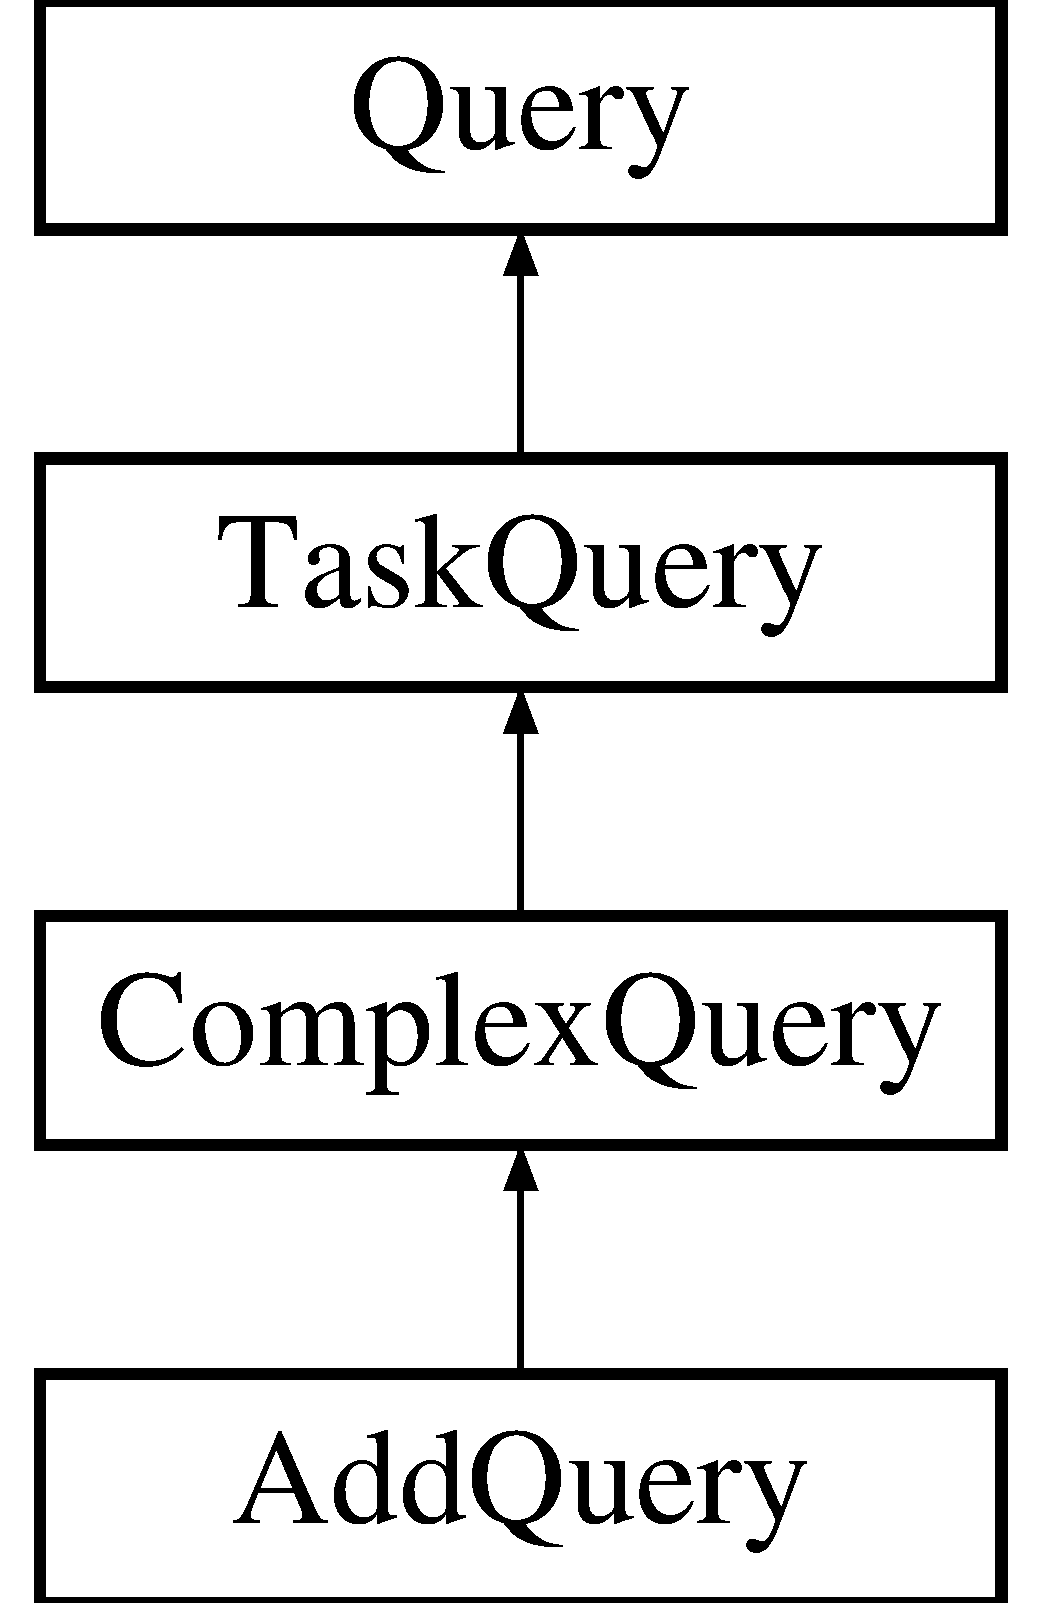
\includegraphics[height=4.000000cm]{class_add_query}
\end{center}
\end{figure}
\subsection*{Public Member Functions}
\begin{DoxyCompactItemize}
\item 
\mbox{\Hypertarget{class_add_query_a6d70d7095946011b69267a16b3cc2f8f}\label{class_add_query_a6d70d7095946011b69267a16b3cc2f8f}} 
{\bfseries L\+E\+M\+O\+N\+D\+B\+\_\+\+Q\+U\+E\+R\+Y\+\_\+\+W\+R\+I\+T\+ER} (true)
\item 
\mbox{\Hypertarget{class_add_query_acc064c75c7141c013b2ba6dcc0effe97}\label{class_add_query_acc064c75c7141c013b2ba6dcc0effe97}} 
Query\+Result\+::\+Ptr {\bfseries execute} () override
\item 
\mbox{\Hypertarget{class_add_query_aad3f5ecd3708f5929e0d4ce44bf6d384}\label{class_add_query_aad3f5ecd3708f5929e0d4ce44bf6d384}} 
std\+::string {\bfseries to\+String} () override
\item 
\mbox{\Hypertarget{class_add_query_aff12e07565e439e191f71bd2caa9f7a9}\label{class_add_query_aff12e07565e439e191f71bd2caa9f7a9}} 
Query\+Result\+::\+Ptr {\bfseries combine} (int \hyperlink{class_task_query_a3dc3e4c56ddea8ff025239fd9da358d3}{task\+Complete}) override
\end{DoxyCompactItemize}
\subsection*{Protected Member Functions}
\begin{DoxyCompactItemize}
\item 
\mbox{\Hypertarget{class_add_query_adaf7f0b6b7c853e217941816d3db7164}\label{class_add_query_adaf7f0b6b7c853e217941816d3db7164}} 
{\bfseries L\+E\+M\+O\+N\+D\+B\+\_\+\+T\+A\+S\+K\+\_\+\+P\+T\+R\+\_\+\+D\+EF} (\hyperlink{class_add_task}{Add\+Task})
\end{DoxyCompactItemize}
\subsection*{Friends}
\begin{DoxyCompactItemize}
\item 
\mbox{\Hypertarget{class_add_query_ae06ff1c286377c113fd46a2c075245e1}\label{class_add_query_ae06ff1c286377c113fd46a2c075245e1}} 
class {\bfseries Add\+Task}
\end{DoxyCompactItemize}
\subsection*{Additional Inherited Members}


\subsection{Detailed Description}


Definition at line 9 of file add\+\_\+query.\+h.



The documentation for this class was generated from the following files\+:\begin{DoxyCompactItemize}
\item 
src/query/data/add\+\_\+query.\+h\item 
src/query/data/add\+\_\+query.\+cpp\end{DoxyCompactItemize}

\hypertarget{class_add_task}{}\section{Add\+Task Class Reference}
\label{class_add_task}\index{Add\+Task@{Add\+Task}}
Inheritance diagram for Add\+Task\+:\begin{figure}[H]
\begin{center}
\leavevmode
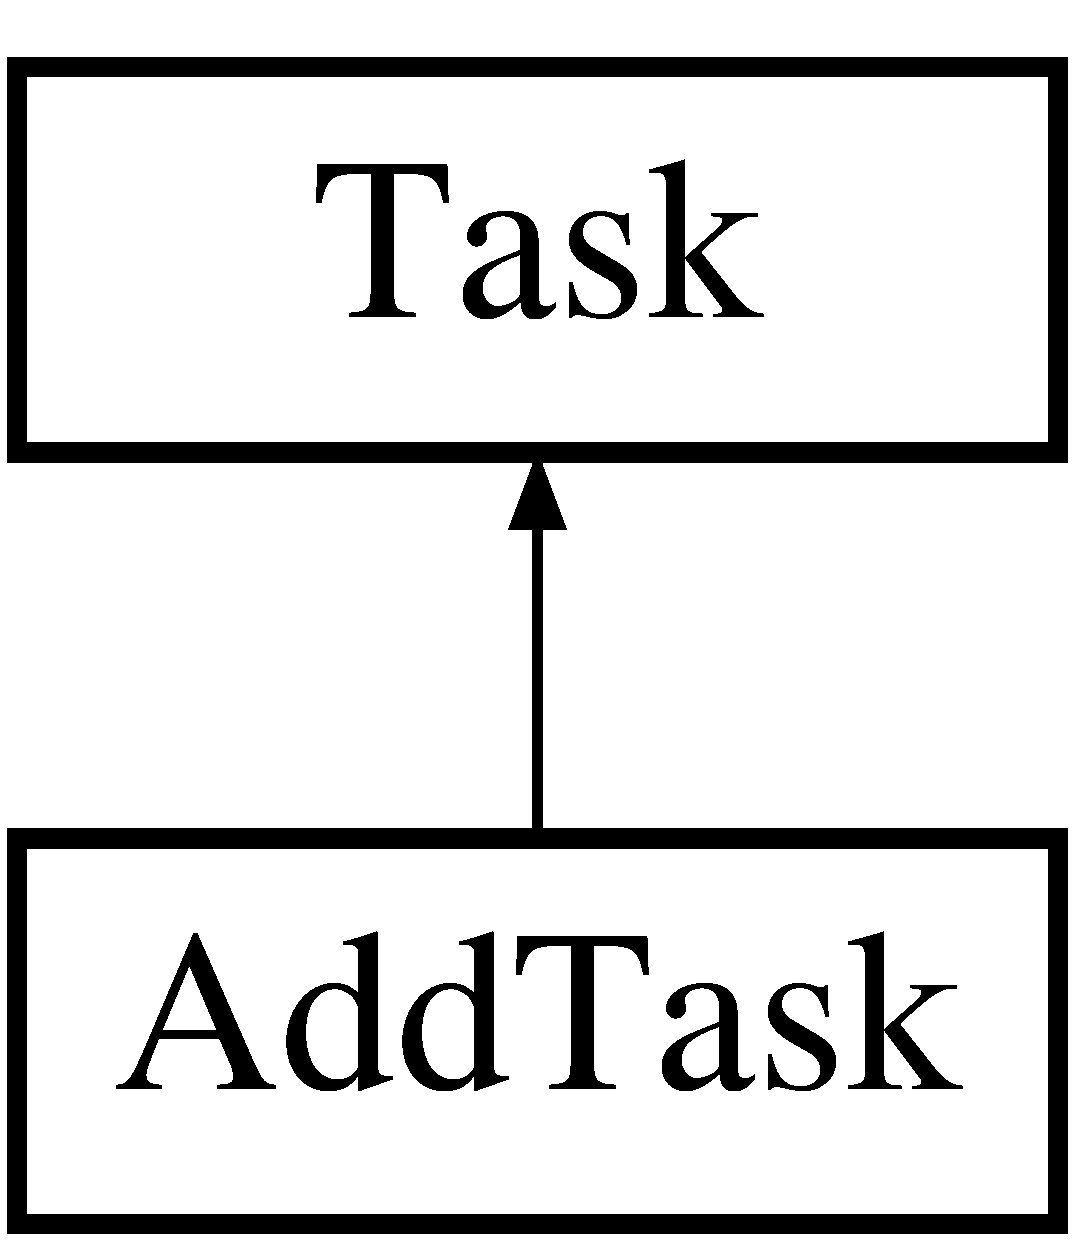
\includegraphics[height=2.000000cm]{class_add_task}
\end{center}
\end{figure}
\subsection*{Public Member Functions}
\begin{DoxyCompactItemize}
\item 
\mbox{\Hypertarget{class_add_task_afd139b27092b495652604e10bd372327}\label{class_add_task_afd139b27092b495652604e10bd372327}} 
void {\bfseries execute} () override
\end{DoxyCompactItemize}
\subsection*{Protected Member Functions}
\begin{DoxyCompactItemize}
\item 
\mbox{\Hypertarget{class_add_task_a46f3795c2a5e96628cd200396100a514}\label{class_add_task_a46f3795c2a5e96628cd200396100a514}} 
{\bfseries L\+E\+M\+O\+N\+D\+B\+\_\+\+Q\+U\+E\+R\+Y\+\_\+\+P\+TR} (\hyperlink{class_add_query}{Add\+Query})
\end{DoxyCompactItemize}
\subsection*{Friends}
\begin{DoxyCompactItemize}
\item 
\mbox{\Hypertarget{class_add_task_a63588833e6226fd09c197a1938e1f753}\label{class_add_task_a63588833e6226fd09c197a1938e1f753}} 
class {\bfseries Add\+Query}
\end{DoxyCompactItemize}
\subsection*{Additional Inherited Members}


\subsection{Detailed Description}


Definition at line 23 of file add\+\_\+query.\+h.



The documentation for this class was generated from the following files\+:\begin{DoxyCompactItemize}
\item 
src/query/data/add\+\_\+query.\+h\item 
src/query/data/add\+\_\+query.\+cpp\end{DoxyCompactItemize}

\hypertarget{class_answer_result}{}\section{Answer\+Result Class Reference}
\label{class_answer_result}\index{Answer\+Result@{Answer\+Result}}
Inheritance diagram for Answer\+Result\+:\begin{figure}[H]
\begin{center}
\leavevmode
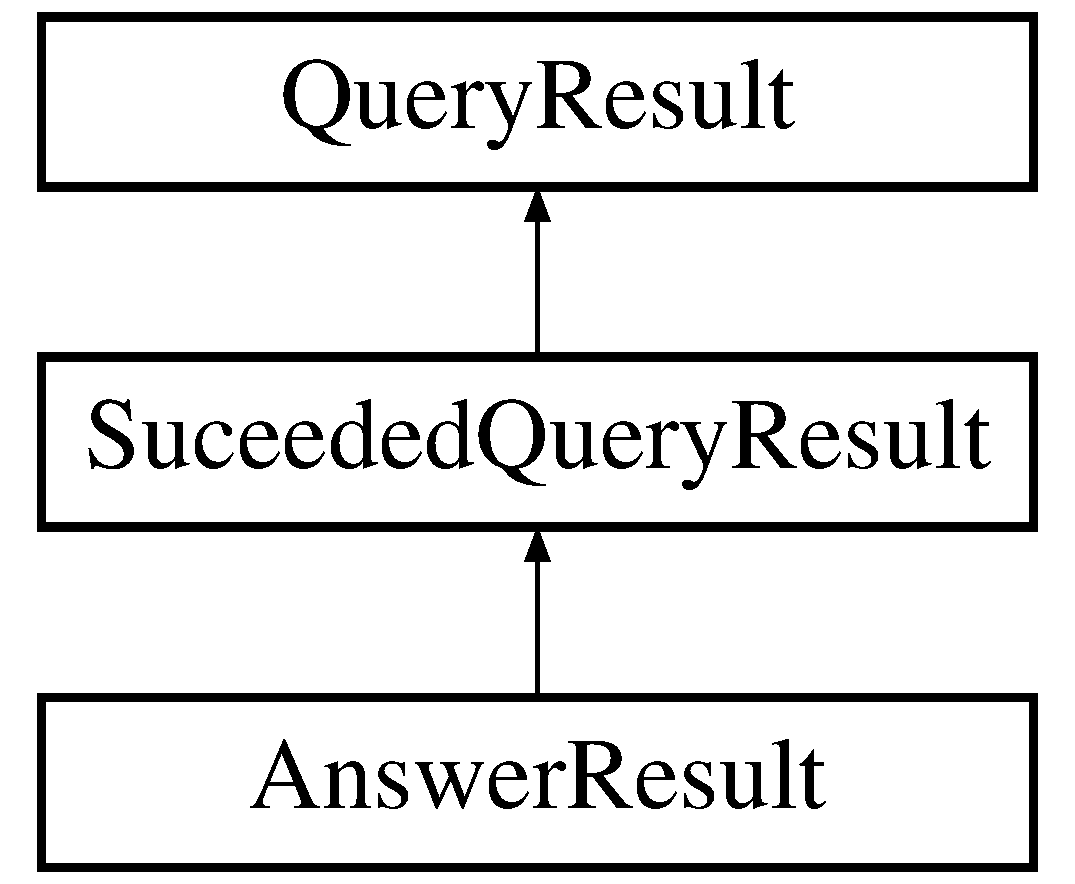
\includegraphics[height=3.000000cm]{class_answer_result}
\end{center}
\end{figure}
\subsection*{Public Member Functions}
\begin{DoxyCompactItemize}
\item 
\mbox{\Hypertarget{class_answer_result_a2e447348660da65b3f8d22cee2666b19}\label{class_answer_result_a2e447348660da65b3f8d22cee2666b19}} 
{\bfseries Answer\+Result} (std\+::vector$<$ int $>$ \&\&answer)
\item 
\mbox{\Hypertarget{class_answer_result_ab8ae0b845ea1aa32d8d86553e9dbd71b}\label{class_answer_result_ab8ae0b845ea1aa32d8d86553e9dbd71b}} 
{\bfseries Answer\+Result} (int answer)
\item 
\mbox{\Hypertarget{class_answer_result_aefaade9c11adfcbe0aae4e4296658cbd}\label{class_answer_result_aefaade9c11adfcbe0aae4e4296658cbd}} 
std\+::string {\bfseries to\+String} () override
\end{DoxyCompactItemize}
\subsection*{Additional Inherited Members}


\subsection{Detailed Description}


Definition at line 108 of file query\+\_\+results.\+h.



The documentation for this class was generated from the following file\+:\begin{DoxyCompactItemize}
\item 
src/query\+\_\+results.\+h\end{DoxyCompactItemize}

\hypertarget{class_basic_query_builder}{}\section{Basic\+Query\+Builder Class Reference}
\label{class_basic_query_builder}\index{Basic\+Query\+Builder@{Basic\+Query\+Builder}}
Inheritance diagram for Basic\+Query\+Builder\+:\begin{figure}[H]
\begin{center}
\leavevmode
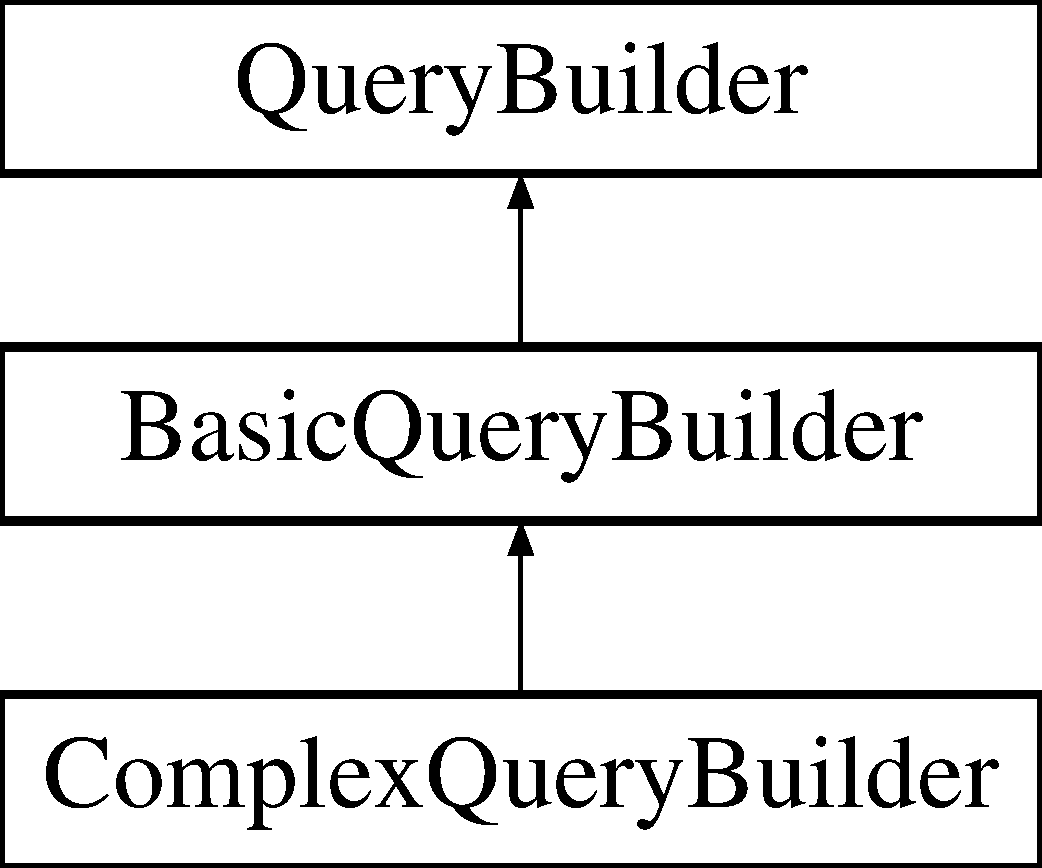
\includegraphics[height=3.000000cm]{class_basic_query_builder}
\end{center}
\end{figure}
\subsection*{Public Member Functions}
\begin{DoxyCompactItemize}
\item 
\mbox{\Hypertarget{class_basic_query_builder_a6f58c9f285534e2328181b7c68246280}\label{class_basic_query_builder_a6f58c9f285534e2328181b7c68246280}} 
void {\bfseries set\+Next} (Ptr \&\&builder) override
\item 
\mbox{\Hypertarget{class_basic_query_builder_a3e8fdcf7b700314b4375c2e46a4499b4}\label{class_basic_query_builder_a3e8fdcf7b700314b4375c2e46a4499b4}} 
Query\+::\+Ptr {\bfseries try\+Extract\+Query} (\hyperlink{struct_tokenized_query_string}{Tokenized\+Query\+String} \&query) override
\item 
\mbox{\Hypertarget{class_basic_query_builder_ad519076333d8b586fa75cc6a4f65379e}\label{class_basic_query_builder_ad519076333d8b586fa75cc6a4f65379e}} 
void {\bfseries clear} () override
\end{DoxyCompactItemize}
\subsection*{Protected Attributes}
\begin{DoxyCompactItemize}
\item 
\mbox{\Hypertarget{class_basic_query_builder_a65dcd7fb6b9e9c468124c75740750718}\label{class_basic_query_builder_a65dcd7fb6b9e9c468124c75740750718}} 
Query\+Builder\+::\+Ptr {\bfseries next\+Builder}
\end{DoxyCompactItemize}
\subsection*{Additional Inherited Members}


\subsection{Detailed Description}


Definition at line 41 of file query\+\_\+builders.\+h.



The documentation for this class was generated from the following file\+:\begin{DoxyCompactItemize}
\item 
src/query\+\_\+builders.\+h\end{DoxyCompactItemize}

\hypertarget{class_complex_query}{}\section{Complex\+Query Class Reference}
\label{class_complex_query}\index{Complex\+Query@{Complex\+Query}}
Inheritance diagram for Complex\+Query\+:\begin{figure}[H]
\begin{center}
\leavevmode
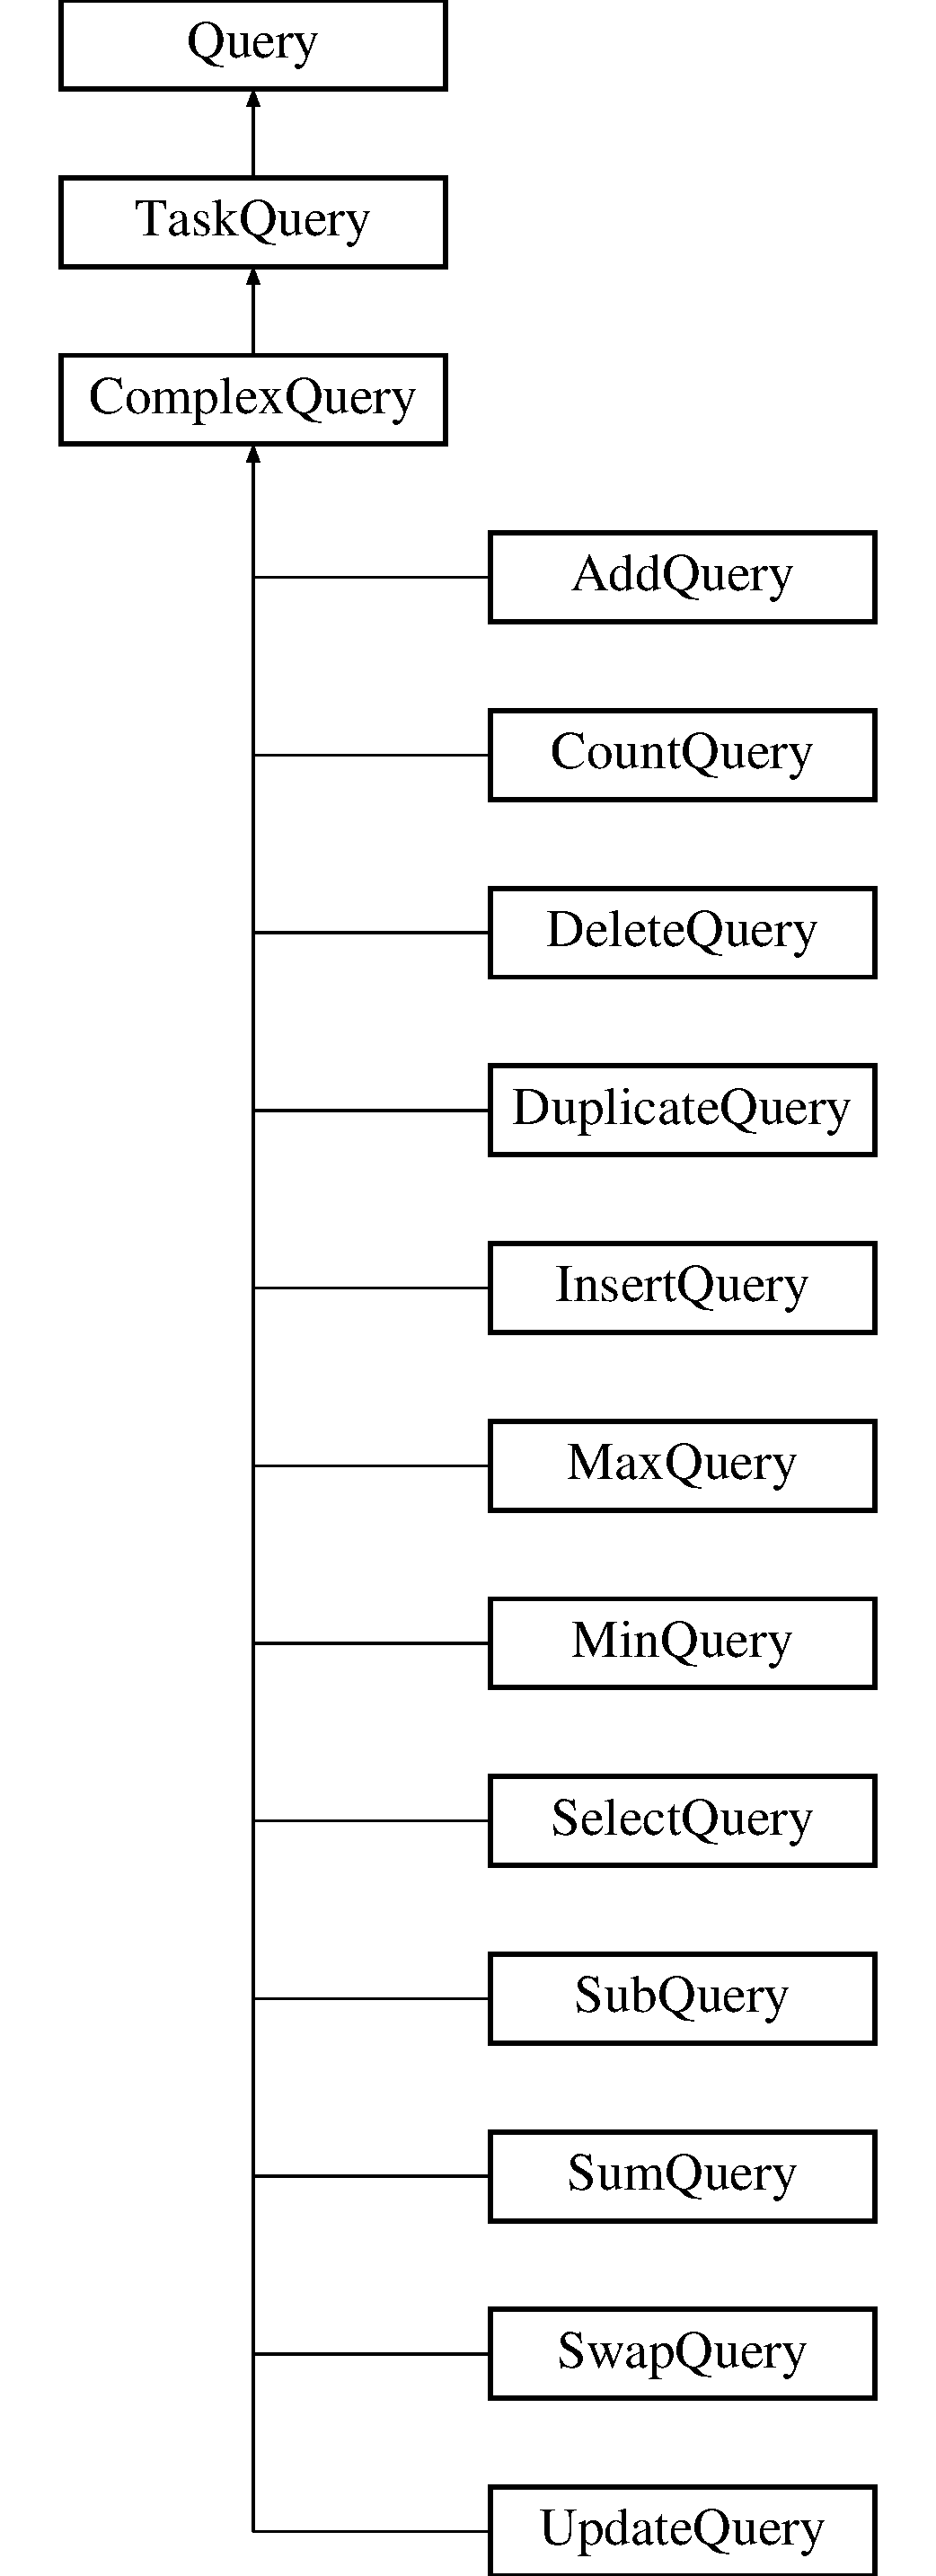
\includegraphics[height=12.000000cm]{class_complex_query}
\end{center}
\end{figure}
\subsection*{Public Types}
\begin{DoxyCompactItemize}
\item 
\mbox{\Hypertarget{class_complex_query_a713f4580157fdd4a058b891599d5347e}\label{class_complex_query_a713f4580157fdd4a058b891599d5347e}} 
typedef std\+::unique\+\_\+ptr$<$ \hyperlink{class_complex_query}{Complex\+Query} $>$ {\bfseries Ptr}
\end{DoxyCompactItemize}
\subsection*{Public Member Functions}
\begin{DoxyCompactItemize}
\item 
std\+::pair$<$ std\+::string, bool $>$ \hyperlink{class_complex_query_af4a16c28edc5ecc3631ef528349279af}{init\+Condition} (const \hyperlink{class_table}{Table} \&table)
\item 
bool \hyperlink{class_complex_query_ae6d00834afbcbe7322b5d7c2fee11e1e}{eval\+Condition} (const \hyperlink{class_table_1_1_object_impl}{Table\+::\+Object} \&object)
\item 
bool \hyperlink{class_complex_query_a111c6bb74ca841541a89c68c4e6a641f}{test\+Key\+Condition} (\hyperlink{class_table}{Table} \&table, std\+::function$<$ void(bool, Table\+::\+Object\+::\+Ptr \&\&)$>$ function)
\item 
\mbox{\Hypertarget{class_complex_query_a5988043a8ce728b0d7740706c5cac9fd}\label{class_complex_query_a5988043a8ce728b0d7740706c5cac9fd}} 
{\bfseries Complex\+Query} (std\+::string target\+Table, std\+::vector$<$ std\+::string $>$ \hyperlink{class_complex_query_a00f38ae7b87fefa8668d7bac95addd94}{operands}, std\+::vector$<$ \hyperlink{struct_query_condition}{Query\+Condition} $>$ \hyperlink{class_complex_query_ac65a30ad8b99278b03d6a64ad34a8a75}{condition})
\item 
const std\+::vector$<$ std\+::string $>$ \& \hyperlink{class_complex_query_a8b01ad18d858402ac96ab83e85e5198f}{get\+Operands} () const
\item 
const std\+::vector$<$ \hyperlink{struct_query_condition}{Query\+Condition} $>$ \& \hyperlink{class_complex_query_a675cc1fc7bbecf1c92698171131fd3c1}{get\+Condition} ()
\end{DoxyCompactItemize}
\subsection*{Protected Attributes}
\begin{DoxyCompactItemize}
\item 
std\+::vector$<$ std\+::string $>$ \hyperlink{class_complex_query_a00f38ae7b87fefa8668d7bac95addd94}{operands}
\item 
std\+::vector$<$ \hyperlink{struct_query_condition}{Query\+Condition} $>$ \hyperlink{class_complex_query_ac65a30ad8b99278b03d6a64ad34a8a75}{condition}
\end{DoxyCompactItemize}


\subsection{Detailed Description}


Definition at line 100 of file query.\+h.



\subsection{Member Function Documentation}
\mbox{\Hypertarget{class_complex_query_ae6d00834afbcbe7322b5d7c2fee11e1e}\label{class_complex_query_ae6d00834afbcbe7322b5d7c2fee11e1e}} 
\index{Complex\+Query@{Complex\+Query}!eval\+Condition@{eval\+Condition}}
\index{eval\+Condition@{eval\+Condition}!Complex\+Query@{Complex\+Query}}
\subsubsection{\texorpdfstring{eval\+Condition()}{evalCondition()}}
{\footnotesize\ttfamily bool Complex\+Query\+::eval\+Condition (\begin{DoxyParamCaption}\item[{const \hyperlink{class_table_1_1_object_impl}{Table\+::\+Object} \&}]{object }\end{DoxyParamCaption})}

skip the evaluation of K\+EY (which should be done after init\+Condition\+Fast is called) 
\begin{DoxyParams}{Parameters}
{\em conditions} & \\
\hline
{\em object} & \\
\hline
\end{DoxyParams}
\begin{DoxyReturn}{Returns}

\end{DoxyReturn}


Definition at line 101 of file query.\+cpp.

\mbox{\Hypertarget{class_complex_query_a675cc1fc7bbecf1c92698171131fd3c1}\label{class_complex_query_a675cc1fc7bbecf1c92698171131fd3c1}} 
\index{Complex\+Query@{Complex\+Query}!get\+Condition@{get\+Condition}}
\index{get\+Condition@{get\+Condition}!Complex\+Query@{Complex\+Query}}
\subsubsection{\texorpdfstring{get\+Condition()}{getCondition()}}
{\footnotesize\ttfamily const std\+::vector$<$\hyperlink{struct_query_condition}{Query\+Condition}$>$\& Complex\+Query\+::get\+Condition (\begin{DoxyParamCaption}{ }\end{DoxyParamCaption})\hspace{0.3cm}{\ttfamily [inline]}}

Get condition in the query, seems no use now 

Definition at line 150 of file query.\+h.

\mbox{\Hypertarget{class_complex_query_a8b01ad18d858402ac96ab83e85e5198f}\label{class_complex_query_a8b01ad18d858402ac96ab83e85e5198f}} 
\index{Complex\+Query@{Complex\+Query}!get\+Operands@{get\+Operands}}
\index{get\+Operands@{get\+Operands}!Complex\+Query@{Complex\+Query}}
\subsubsection{\texorpdfstring{get\+Operands()}{getOperands()}}
{\footnotesize\ttfamily const std\+::vector$<$std\+::string$>$\& Complex\+Query\+::get\+Operands (\begin{DoxyParamCaption}{ }\end{DoxyParamCaption}) const\hspace{0.3cm}{\ttfamily [inline]}}

Get operands in the query 

Definition at line 147 of file query.\+h.

\mbox{\Hypertarget{class_complex_query_af4a16c28edc5ecc3631ef528349279af}\label{class_complex_query_af4a16c28edc5ecc3631ef528349279af}} 
\index{Complex\+Query@{Complex\+Query}!init\+Condition@{init\+Condition}}
\index{init\+Condition@{init\+Condition}!Complex\+Query@{Complex\+Query}}
\subsubsection{\texorpdfstring{init\+Condition()}{initCondition()}}
{\footnotesize\ttfamily std\+::pair$<$ std\+::string, bool $>$ Complex\+Query\+::init\+Condition (\begin{DoxyParamCaption}\item[{const \hyperlink{class_table}{Table} \&}]{table }\end{DoxyParamCaption})}

init a fast condition according to the table note that the condition is only effective if the table fields are not changed 
\begin{DoxyParams}{Parameters}
{\em table} & \\
\hline
{\em conditions} & \\
\hline
\end{DoxyParams}
\begin{DoxyReturn}{Returns}
a pair of the key and a flag if flag is false, the condition is always false in this situation, the condition may not be fully initialized to save time 
\end{DoxyReturn}


Definition at line 45 of file query.\+cpp.

\mbox{\Hypertarget{class_complex_query_a111c6bb74ca841541a89c68c4e6a641f}\label{class_complex_query_a111c6bb74ca841541a89c68c4e6a641f}} 
\index{Complex\+Query@{Complex\+Query}!test\+Key\+Condition@{test\+Key\+Condition}}
\index{test\+Key\+Condition@{test\+Key\+Condition}!Complex\+Query@{Complex\+Query}}
\subsubsection{\texorpdfstring{test\+Key\+Condition()}{testKeyCondition()}}
{\footnotesize\ttfamily bool Complex\+Query\+::test\+Key\+Condition (\begin{DoxyParamCaption}\item[{\hyperlink{class_table}{Table} \&}]{table,  }\item[{std\+::function$<$ void(bool, Table\+::\+Object\+::\+Ptr \&\&)$>$}]{function }\end{DoxyParamCaption})}

This function seems have small effect and causes somme bugs so it is not used actually 
\begin{DoxyParams}{Parameters}
{\em table} & \\
\hline
{\em function} & \\
\hline
\end{DoxyParams}
\begin{DoxyReturn}{Returns}

\end{DoxyReturn}


Definition at line 113 of file query.\+cpp.



\subsection{Member Data Documentation}
\mbox{\Hypertarget{class_complex_query_ac65a30ad8b99278b03d6a64ad34a8a75}\label{class_complex_query_ac65a30ad8b99278b03d6a64ad34a8a75}} 
\index{Complex\+Query@{Complex\+Query}!condition@{condition}}
\index{condition@{condition}!Complex\+Query@{Complex\+Query}}
\subsubsection{\texorpdfstring{condition}{condition}}
{\footnotesize\ttfamily std\+::vector$<$\hyperlink{struct_query_condition}{Query\+Condition}$>$ Complex\+Query\+::condition\hspace{0.3cm}{\ttfamily [protected]}}

The function used in where clause 

Definition at line 105 of file query.\+h.

\mbox{\Hypertarget{class_complex_query_a00f38ae7b87fefa8668d7bac95addd94}\label{class_complex_query_a00f38ae7b87fefa8668d7bac95addd94}} 
\index{Complex\+Query@{Complex\+Query}!operands@{operands}}
\index{operands@{operands}!Complex\+Query@{Complex\+Query}}
\subsubsection{\texorpdfstring{operands}{operands}}
{\footnotesize\ttfamily std\+::vector$<$std\+::string$>$ Complex\+Query\+::operands\hspace{0.3cm}{\ttfamily [protected]}}

The field names in the first () 

Definition at line 103 of file query.\+h.



The documentation for this class was generated from the following files\+:\begin{DoxyCompactItemize}
\item 
src/query/query.\+h\item 
src/query/query.\+cpp\end{DoxyCompactItemize}

\hypertarget{class_complex_query_builder}{}\section{Complex\+Query\+Builder Class Reference}
\label{class_complex_query_builder}\index{Complex\+Query\+Builder@{Complex\+Query\+Builder}}
Inheritance diagram for Complex\+Query\+Builder\+:\begin{figure}[H]
\begin{center}
\leavevmode
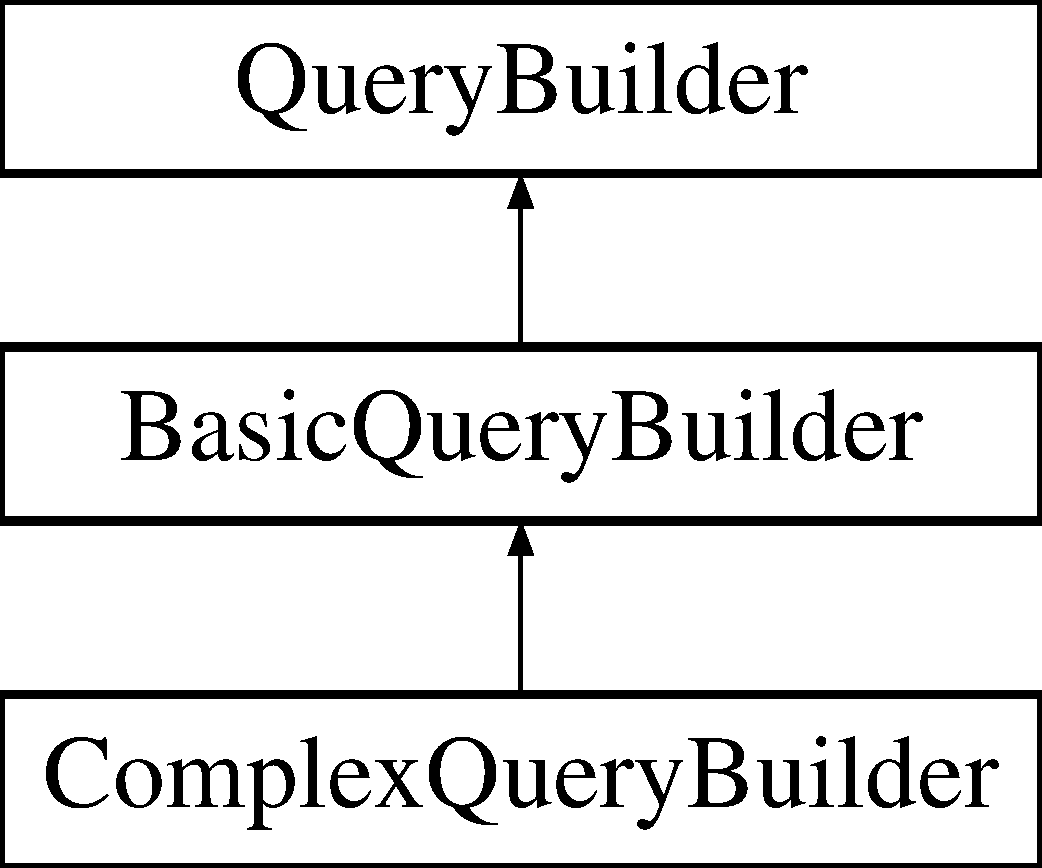
\includegraphics[height=3.000000cm]{class_complex_query_builder}
\end{center}
\end{figure}
\subsection*{Public Member Functions}
\begin{DoxyCompactItemize}
\item 
\mbox{\Hypertarget{class_complex_query_builder_aaf3f971daf43452502fc6fed296494e9}\label{class_complex_query_builder_aaf3f971daf43452502fc6fed296494e9}} 
void {\bfseries clear} () override
\item 
\mbox{\Hypertarget{class_complex_query_builder_aab521c81b6ecb9bc4466a61cdf9ccfed}\label{class_complex_query_builder_aab521c81b6ecb9bc4466a61cdf9ccfed}} 
Query\+::\+Ptr {\bfseries try\+Extract\+Query} (\hyperlink{struct_tokenized_query_string}{Tokenized\+Query\+String} \&query) override
\end{DoxyCompactItemize}
\subsection*{Protected Member Functions}
\begin{DoxyCompactItemize}
\item 
\mbox{\Hypertarget{class_complex_query_builder_a1169df1b39a76c283bea1f0f7ec601d9}\label{class_complex_query_builder_a1169df1b39a76c283bea1f0f7ec601d9}} 
virtual void {\bfseries parse\+Token} (\hyperlink{struct_tokenized_query_string}{Tokenized\+Query\+String} \&query)
\end{DoxyCompactItemize}
\subsection*{Protected Attributes}
\begin{DoxyCompactItemize}
\item 
\mbox{\Hypertarget{class_complex_query_builder_ae8285f6ee5ac598c2593411badf674b7}\label{class_complex_query_builder_ae8285f6ee5ac598c2593411badf674b7}} 
std\+::string {\bfseries target\+Table}
\item 
\mbox{\Hypertarget{class_complex_query_builder_a40cee0c08e7fc932cd1a2d418d23da94}\label{class_complex_query_builder_a40cee0c08e7fc932cd1a2d418d23da94}} 
std\+::vector$<$ std\+::string $>$ {\bfseries operand\+Token}
\item 
\mbox{\Hypertarget{class_complex_query_builder_aa230f7984124087dba13a40f16d1c5a7}\label{class_complex_query_builder_aa230f7984124087dba13a40f16d1c5a7}} 
std\+::vector$<$ \hyperlink{struct_query_condition}{Query\+Condition} $>$ {\bfseries condition\+Token}
\end{DoxyCompactItemize}
\subsection*{Additional Inherited Members}


\subsection{Detailed Description}


Definition at line 60 of file query\+\_\+builders.\+h.



The documentation for this class was generated from the following files\+:\begin{DoxyCompactItemize}
\item 
src/query\+\_\+builders.\+h\item 
src/query\+\_\+builders.\+cpp\end{DoxyCompactItemize}

\hypertarget{struct_conflicting_key}{}\section{Conflicting\+Key Struct Reference}
\label{struct_conflicting_key}\index{Conflicting\+Key@{Conflicting\+Key}}
Inheritance diagram for Conflicting\+Key\+:\begin{figure}[H]
\begin{center}
\leavevmode
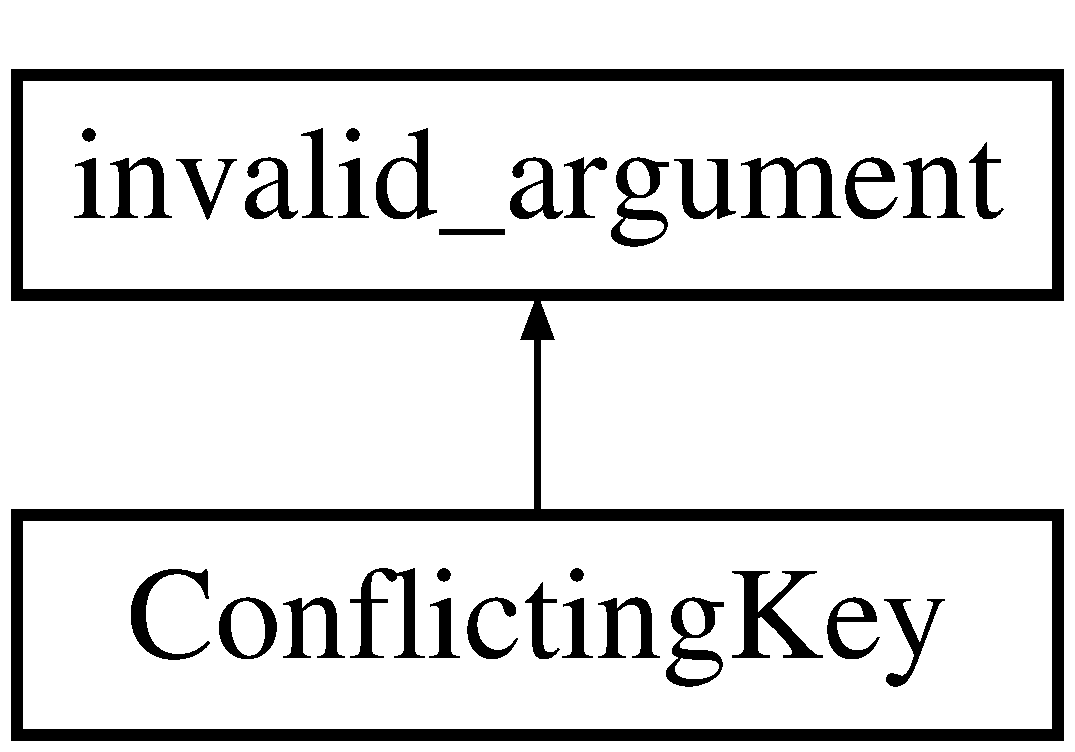
\includegraphics[height=2.000000cm]{struct_conflicting_key}
\end{center}
\end{figure}
\subsection*{Public Member Functions}
\begin{DoxyCompactItemize}
\item 
\mbox{\Hypertarget{struct_conflicting_key_ac87d5c5f7fde32f966407684ef3c3d98}\label{struct_conflicting_key_ac87d5c5f7fde32f966407684ef3c3d98}} 
{\bfseries Conflicting\+Key} (const std\+::string \&str)
\end{DoxyCompactItemize}


\subsection{Detailed Description}


Definition at line 26 of file uexception.\+h.



The documentation for this struct was generated from the following file\+:\begin{DoxyCompactItemize}
\item 
src/uexception.\+h\end{DoxyCompactItemize}

\hypertarget{class_copy_table_dest_query}{}\section{Copy\+Table\+Dest\+Query Class Reference}
\label{class_copy_table_dest_query}\index{Copy\+Table\+Dest\+Query@{Copy\+Table\+Dest\+Query}}
Inheritance diagram for Copy\+Table\+Dest\+Query\+:\begin{figure}[H]
\begin{center}
\leavevmode
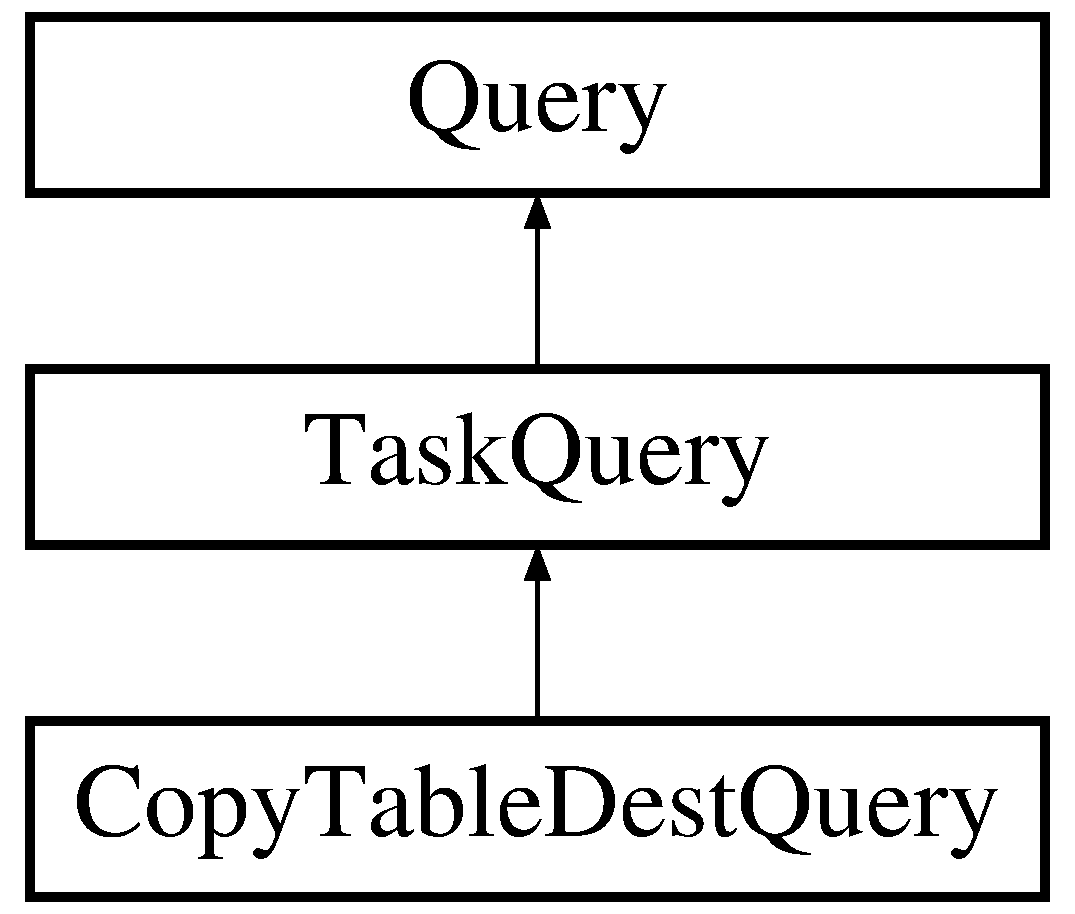
\includegraphics[height=3.000000cm]{class_copy_table_dest_query}
\end{center}
\end{figure}
\subsection*{Public Member Functions}
\begin{DoxyCompactItemize}
\item 
\mbox{\Hypertarget{class_copy_table_dest_query_a0330ab9aec75378c99446501fac4e7f8}\label{class_copy_table_dest_query_a0330ab9aec75378c99446501fac4e7f8}} 
{\bfseries L\+E\+M\+O\+N\+D\+B\+\_\+\+Q\+U\+E\+R\+Y\+\_\+\+W\+R\+I\+T\+ER} (true)
\item 
\mbox{\Hypertarget{class_copy_table_dest_query_a265356fa4dc7ee9e8fb4acf20a3aec3c}\label{class_copy_table_dest_query_a265356fa4dc7ee9e8fb4acf20a3aec3c}} 
{\bfseries L\+E\+M\+O\+N\+D\+B\+\_\+\+Q\+U\+E\+R\+Y\+\_\+\+I\+N\+S\+T\+A\+NT} (true)
\item 
\mbox{\Hypertarget{class_copy_table_dest_query_a3e78494953a88aeed13c482d1f426778}\label{class_copy_table_dest_query_a3e78494953a88aeed13c482d1f426778}} 
{\bfseries Copy\+Table\+Dest\+Query} (std\+::string table, \hyperlink{class_copy_table_query}{Copy\+Table\+Query} $\ast$src\+Query)
\item 
\mbox{\Hypertarget{class_copy_table_dest_query_aebf279d8567c5a6124ac151a67f757b3}\label{class_copy_table_dest_query_aebf279d8567c5a6124ac151a67f757b3}} 
Query\+Result\+::\+Ptr {\bfseries execute} () override
\item 
\mbox{\Hypertarget{class_copy_table_dest_query_a87dbf6553887c701dadb613ed1501e34}\label{class_copy_table_dest_query_a87dbf6553887c701dadb613ed1501e34}} 
std\+::string {\bfseries to\+String} () override
\end{DoxyCompactItemize}
\subsection*{Friends}
\begin{DoxyCompactItemize}
\item 
\mbox{\Hypertarget{class_copy_table_dest_query_ac6745199122174064b06f954a6eb3ec3}\label{class_copy_table_dest_query_ac6745199122174064b06f954a6eb3ec3}} 
class {\bfseries Copy\+Table\+Query}
\end{DoxyCompactItemize}
\subsection*{Additional Inherited Members}


\subsection{Detailed Description}


Definition at line 26 of file copy\+\_\+table\+\_\+query.\+h.



The documentation for this class was generated from the following files\+:\begin{DoxyCompactItemize}
\item 
src/query/management/copy\+\_\+table\+\_\+query.\+h\item 
src/query/management/copy\+\_\+table\+\_\+query.\+cpp\end{DoxyCompactItemize}

\hypertarget{class_copy_table_query}{}\section{Copy\+Table\+Query Class Reference}
\label{class_copy_table_query}\index{Copy\+Table\+Query@{Copy\+Table\+Query}}
Inheritance diagram for Copy\+Table\+Query\+:\begin{figure}[H]
\begin{center}
\leavevmode
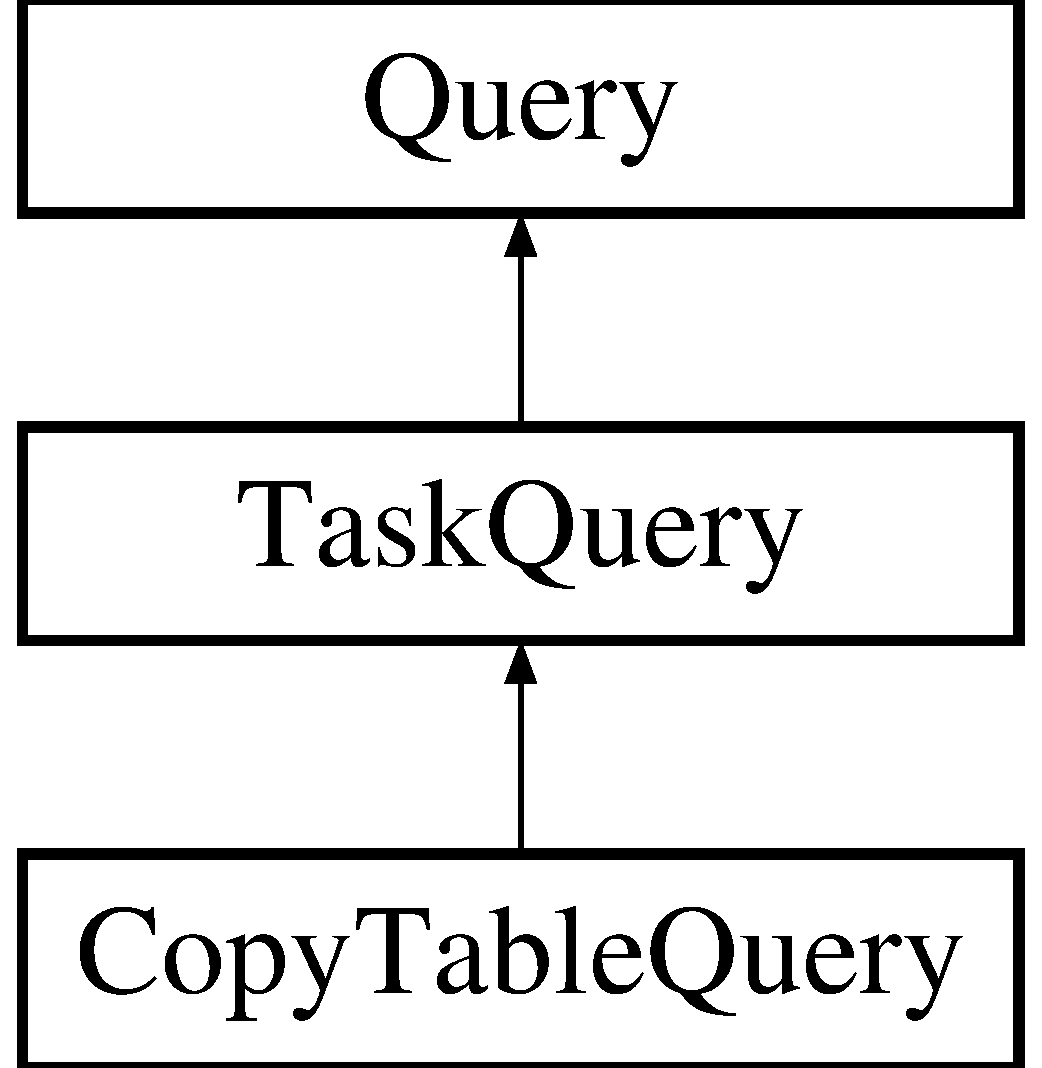
\includegraphics[height=3.000000cm]{class_copy_table_query}
\end{center}
\end{figure}
\subsection*{Public Member Functions}
\begin{DoxyCompactItemize}
\item 
\mbox{\Hypertarget{class_copy_table_query_adb7ceaaa450b6a126680cc2f87028233}\label{class_copy_table_query_adb7ceaaa450b6a126680cc2f87028233}} 
{\bfseries L\+E\+M\+O\+N\+D\+B\+\_\+\+Q\+U\+E\+R\+Y\+\_\+\+W\+R\+I\+T\+ER} (false)
\item 
\mbox{\Hypertarget{class_copy_table_query_a79430091766721db1b8c706f76582b73}\label{class_copy_table_query_a79430091766721db1b8c706f76582b73}} 
{\bfseries Copy\+Table\+Query} (std\+::string table, std\+::string new\+Table)
\item 
\mbox{\Hypertarget{class_copy_table_query_a8d360d5ba13351124ed9a6114c20fb10}\label{class_copy_table_query_a8d360d5ba13351124ed9a6114c20fb10}} 
Query\+Result\+::\+Ptr {\bfseries execute} () override
\item 
\mbox{\Hypertarget{class_copy_table_query_ae6b92734e8e8121e4360073bc7d8a54a}\label{class_copy_table_query_ae6b92734e8e8121e4360073bc7d8a54a}} 
std\+::string {\bfseries to\+String} () override
\item 
\mbox{\Hypertarget{class_copy_table_query_a9291c277d7cfb790849551a7a7cc0ccc}\label{class_copy_table_query_a9291c277d7cfb790849551a7a7cc0ccc}} 
Query\+::\+Ptr {\bfseries create\+Dest\+Query} ()
\end{DoxyCompactItemize}
\subsection*{Additional Inherited Members}


\subsection{Detailed Description}


Definition at line 13 of file copy\+\_\+table\+\_\+query.\+h.



The documentation for this class was generated from the following files\+:\begin{DoxyCompactItemize}
\item 
src/query/management/copy\+\_\+table\+\_\+query.\+h\item 
src/query/management/copy\+\_\+table\+\_\+query.\+cpp\end{DoxyCompactItemize}

\hypertarget{class_count_query}{}\section{Count\+Query Class Reference}
\label{class_count_query}\index{Count\+Query@{Count\+Query}}
Inheritance diagram for Count\+Query\+:\begin{figure}[H]
\begin{center}
\leavevmode
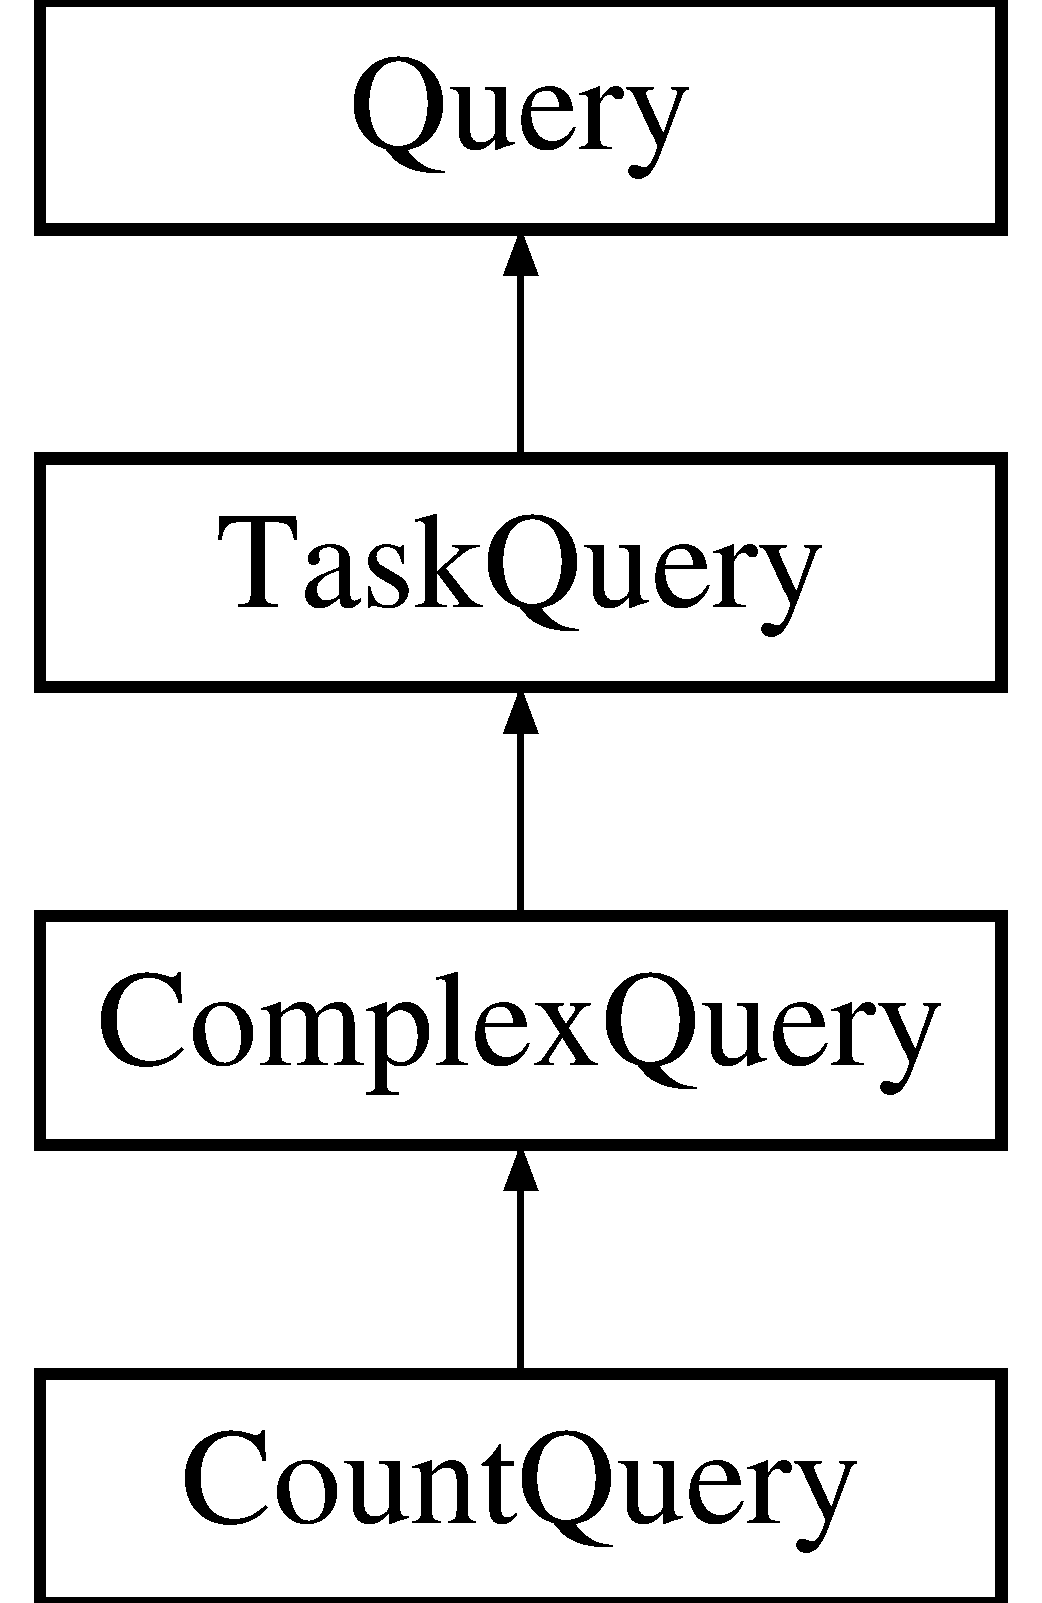
\includegraphics[height=4.000000cm]{class_count_query}
\end{center}
\end{figure}
\subsection*{Public Member Functions}
\begin{DoxyCompactItemize}
\item 
\mbox{\Hypertarget{class_count_query_a00049389ec33e0dbbf931154f3c1e29a}\label{class_count_query_a00049389ec33e0dbbf931154f3c1e29a}} 
{\bfseries L\+E\+M\+O\+N\+D\+B\+\_\+\+Q\+U\+E\+R\+Y\+\_\+\+W\+R\+I\+T\+ER} (false)
\item 
\mbox{\Hypertarget{class_count_query_a4a5b116eb6efe197d765181e0f9913c0}\label{class_count_query_a4a5b116eb6efe197d765181e0f9913c0}} 
Query\+Result\+::\+Ptr {\bfseries execute} () override
\item 
\mbox{\Hypertarget{class_count_query_a23cf22e71dc52c0cf61eecdc01ca9dea}\label{class_count_query_a23cf22e71dc52c0cf61eecdc01ca9dea}} 
std\+::string {\bfseries to\+String} () override
\item 
\mbox{\Hypertarget{class_count_query_a6eea6ab67e3b1f5d0589a47207192002}\label{class_count_query_a6eea6ab67e3b1f5d0589a47207192002}} 
Query\+Result\+::\+Ptr {\bfseries combine} (int \hyperlink{class_task_query_a3dc3e4c56ddea8ff025239fd9da358d3}{task\+Complete}) override
\end{DoxyCompactItemize}
\subsection*{Additional Inherited Members}


\subsection{Detailed Description}


Definition at line 7 of file count\+\_\+query.\+h.



The documentation for this class was generated from the following files\+:\begin{DoxyCompactItemize}
\item 
src/query/data/count\+\_\+query.\+h\item 
src/query/data/count\+\_\+query.\+cpp\end{DoxyCompactItemize}

\hypertarget{class_count_task}{}\section{Count\+Task Class Reference}
\label{class_count_task}\index{Count\+Task@{Count\+Task}}
Inheritance diagram for Count\+Task\+:\begin{figure}[H]
\begin{center}
\leavevmode
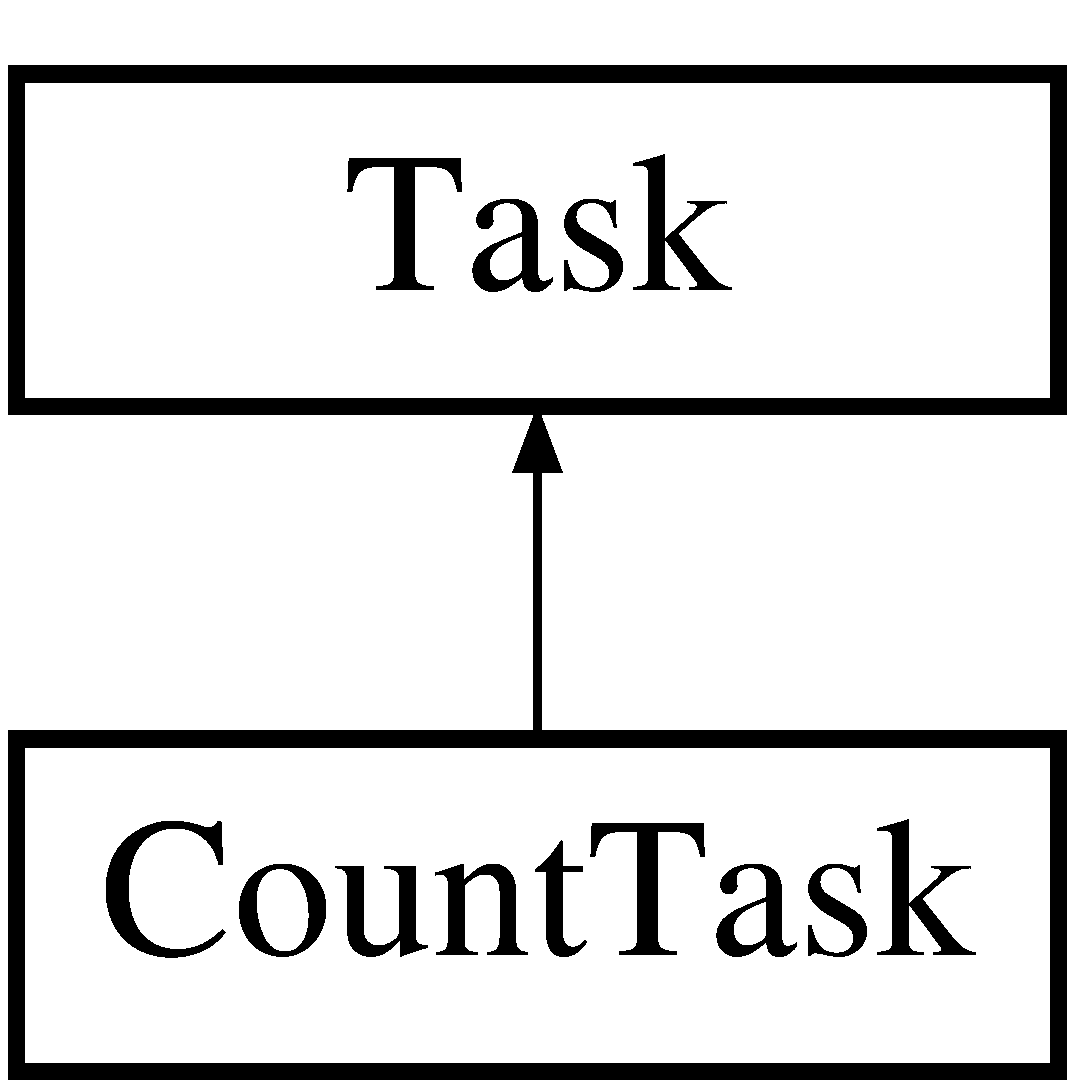
\includegraphics[height=2.000000cm]{class_count_task}
\end{center}
\end{figure}
\subsection*{Public Member Functions}
\begin{DoxyCompactItemize}
\item 
\mbox{\Hypertarget{class_count_task_a78489ba36acf7f88bbb87cc138872748}\label{class_count_task_a78489ba36acf7f88bbb87cc138872748}} 
void {\bfseries execute} () override
\end{DoxyCompactItemize}
\subsection*{Protected Member Functions}
\begin{DoxyCompactItemize}
\item 
\mbox{\Hypertarget{class_count_task_ad53272fd6ecb1fb5e7176bcfcf39b037}\label{class_count_task_ad53272fd6ecb1fb5e7176bcfcf39b037}} 
{\bfseries L\+E\+M\+O\+N\+D\+B\+\_\+\+Q\+U\+E\+R\+Y\+\_\+\+P\+TR} (\hyperlink{class_count_query}{Count\+Query})
\end{DoxyCompactItemize}
\subsection*{Additional Inherited Members}


\subsection{Detailed Description}


Definition at line 17 of file count\+\_\+query.\+h.



The documentation for this class was generated from the following files\+:\begin{DoxyCompactItemize}
\item 
src/query/data/count\+\_\+query.\+h\item 
src/query/data/count\+\_\+query.\+cpp\end{DoxyCompactItemize}

\hypertarget{class_database}{}\section{Database Class Reference}
\label{class_database}\index{Database@{Database}}
\subsection*{Public Member Functions}
\begin{DoxyCompactItemize}
\item 
\mbox{\Hypertarget{class_database_adc114c831a4569d60c6334a943f48516}\label{class_database_adc114c831a4569d60c6334a943f48516}} 
void {\bfseries register\+Table} (Table\+::\+Ptr \&\&table)
\item 
\hyperlink{class_table}{Table} \& \hyperlink{class_database_a1405a11517ac20b0036514120782cee5}{ensure\+Table} (const std\+::string \&table\+Name)
\item 
\mbox{\Hypertarget{class_database_a95a3310cac23f486f309bcc69fa034a4}\label{class_database_a95a3310cac23f486f309bcc69fa034a4}} 
void {\bfseries drop\+Table} (std\+::string table\+Name)
\item 
\mbox{\Hypertarget{class_database_a6f6dad3936a8cf6274924156fa28c4b7}\label{class_database_a6f6dad3936a8cf6274924156fa28c4b7}} 
void {\bfseries print\+All\+Table} ()
\item 
\mbox{\Hypertarget{class_database_a07b70401d5381678c781f0eb09cfeaa0}\label{class_database_a07b70401d5381678c781f0eb09cfeaa0}} 
\hyperlink{class_table}{Table} \& {\bfseries operator\mbox{[}$\,$\mbox{]}} (std\+::string table\+Name)
\item 
\mbox{\Hypertarget{class_database_a7c76b022a64b9ef07e3255b937d28bea}\label{class_database_a7c76b022a64b9ef07e3255b937d28bea}} 
const \hyperlink{class_table}{Table} \& {\bfseries operator\mbox{[}$\,$\mbox{]}} (std\+::string table\+Name) const
\item 
\mbox{\Hypertarget{class_database_a91a7742eb10d89e79b534ce3d093e40f}\label{class_database_a91a7742eb10d89e79b534ce3d093e40f}} 
\hyperlink{class_database}{Database} \& {\bfseries operator=} (const \hyperlink{class_database}{Database} \&)=delete
\item 
\mbox{\Hypertarget{class_database_a1a54186b16f03c8e6e26b8361fe69ddd}\label{class_database_a1a54186b16f03c8e6e26b8361fe69ddd}} 
\hyperlink{class_database}{Database} \& {\bfseries operator=} (\hyperlink{class_database}{Database} \&\&)=delete
\item 
\mbox{\Hypertarget{class_database_a83f8b6d2941a4aee50f225e08e97291c}\label{class_database_a83f8b6d2941a4aee50f225e08e97291c}} 
{\bfseries Database} (const \hyperlink{class_database}{Database} \&)=delete
\item 
\mbox{\Hypertarget{class_database_a00d16c8b373c9bb4bad59550648c5393}\label{class_database_a00d16c8b373c9bb4bad59550648c5393}} 
{\bfseries Database} (\hyperlink{class_database}{Database} \&\&)=delete
\item 
\mbox{\Hypertarget{class_database_acd5776560ea4d5ab583cceea209bb721}\label{class_database_acd5776560ea4d5ab583cceea209bb721}} 
void {\bfseries update\+File\+Table\+Name} (const std\+::string \&file\+Name, const std\+::string \&table\+Name)
\item 
\mbox{\Hypertarget{class_database_a7819fe58fa0cc1bd3fd35b053be46895}\label{class_database_a7819fe58fa0cc1bd3fd35b053be46895}} 
std\+::string {\bfseries get\+File\+Table\+Name} (const std\+::string \&file\+Name)
\item 
void \hyperlink{class_database_a537758fac6907e4d0f5e136a5c894a3d}{add\+Query} (Query\+::\+Ptr \&\&query)
\item 
void \hyperlink{class_database_a49110ec81b4011c47011ef3b0a348a70}{add\+Task} (\hyperlink{class_task}{Task} $\ast$task)
\item 
\mbox{\Hypertarget{class_database_a3821a8fc52aac97e6cfda234bc257c97}\label{class_database_a3821a8fc52aac97e6cfda234bc257c97}} 
void {\bfseries add\+Result} (\hyperlink{class_query}{Query} $\ast$query, Query\+Result\+::\+Ptr \&\&result)
\item 
void \hyperlink{class_database_a55858cf28c9a4118ac97bdc9a1abf981}{complete\+Query} ()
\item 
\mbox{\Hypertarget{class_database_afbab61ba6d854b086cbe46b9921408f4}\label{class_database_afbab61ba6d854b086cbe46b9921408f4}} 
void {\bfseries end\+Query} ()
\item 
\mbox{\Hypertarget{class_database_a45c9bb61f3ca877def1c97651e1f5a3d}\label{class_database_a45c9bb61f3ca877def1c97651e1f5a3d}} 
bool {\bfseries is\+End} () const
\item 
\mbox{\Hypertarget{class_database_ac7de0114f3bbe1d269a57c398696ecfb}\label{class_database_ac7de0114f3bbe1d269a57c398696ecfb}} 
void {\bfseries join\+Threads} ()
\end{DoxyCompactItemize}
\subsection*{Static Public Member Functions}
\begin{DoxyCompactItemize}
\item 
\mbox{\Hypertarget{class_database_a317c583698e8c788b146144de307df7e}\label{class_database_a317c583698e8c788b146144de307df7e}} 
static \hyperlink{class_database}{Database} \& {\bfseries get\+Instance} ()
\end{DoxyCompactItemize}


\subsection{Detailed Description}


Definition at line 16 of file db.\+h.



\subsection{Member Function Documentation}
\mbox{\Hypertarget{class_database_a537758fac6907e4d0f5e136a5c894a3d}\label{class_database_a537758fac6907e4d0f5e136a5c894a3d}} 
\index{Database@{Database}!add\+Query@{add\+Query}}
\index{add\+Query@{add\+Query}!Database@{Database}}
\subsubsection{\texorpdfstring{add\+Query()}{addQuery()}}
{\footnotesize\ttfamily void Database\+::add\+Query (\begin{DoxyParamCaption}\item[{Query\+::\+Ptr \&\&}]{query }\end{DoxyParamCaption})}

Add a parsed query after reading it dispatch the query according to its target table 
\begin{DoxyParams}{Parameters}
{\em query} & \\
\hline
\end{DoxyParams}


Definition at line 117 of file db.\+cpp.

\mbox{\Hypertarget{class_database_a49110ec81b4011c47011ef3b0a348a70}\label{class_database_a49110ec81b4011c47011ef3b0a348a70}} 
\index{Database@{Database}!add\+Task@{add\+Task}}
\index{add\+Task@{add\+Task}!Database@{Database}}
\subsubsection{\texorpdfstring{add\+Task()}{addTask()}}
{\footnotesize\ttfamily void Database\+::add\+Task (\begin{DoxyParamCaption}\item[{\hyperlink{class_task}{Task} $\ast$}]{task }\end{DoxyParamCaption})}

Add a generated task after a query has been executed by a table idle working threads are waiting for the task 
\begin{DoxyParams}{Parameters}
{\em task} & \\
\hline
\end{DoxyParams}


Definition at line 146 of file db.\+cpp.

\mbox{\Hypertarget{class_database_a55858cf28c9a4118ac97bdc9a1abf981}\label{class_database_a55858cf28c9a4118ac97bdc9a1abf981}} 
\index{Database@{Database}!complete\+Query@{complete\+Query}}
\index{complete\+Query@{complete\+Query}!Database@{Database}}
\subsubsection{\texorpdfstring{complete\+Query()}{completeQuery()}}
{\footnotesize\ttfamily void Database\+::complete\+Query (\begin{DoxyParamCaption}{ }\end{DoxyParamCaption})}

try to output the query result in order 

Definition at line 165 of file db.\+cpp.

\mbox{\Hypertarget{class_database_a1405a11517ac20b0036514120782cee5}\label{class_database_a1405a11517ac20b0036514120782cee5}} 
\index{Database@{Database}!ensure\+Table@{ensure\+Table}}
\index{ensure\+Table@{ensure\+Table}!Database@{Database}}
\subsubsection{\texorpdfstring{ensure\+Table()}{ensureTable()}}
{\footnotesize\ttfamily \hyperlink{class_table}{Table} \& Database\+::ensure\+Table (\begin{DoxyParamCaption}\item[{const std\+::string \&}]{table\+Name }\end{DoxyParamCaption})}

get the table if it already exists create a table if table\+Name not found use tables\+Mutex, call it when needed if table\+Name must exist, use operator\mbox{[}\mbox{]} 
\begin{DoxyParams}{Parameters}
{\em table\+Name} & \\
\hline
\end{DoxyParams}
\begin{DoxyReturn}{Returns}

\end{DoxyReturn}


Definition at line 43 of file db.\+cpp.



The documentation for this class was generated from the following files\+:\begin{DoxyCompactItemize}
\item 
src/db/db.\+h\item 
src/db/db.\+cpp\end{DoxyCompactItemize}

\hypertarget{class_delete_query}{}\section{Delete\+Query Class Reference}
\label{class_delete_query}\index{Delete\+Query@{Delete\+Query}}
Inheritance diagram for Delete\+Query\+:\begin{figure}[H]
\begin{center}
\leavevmode
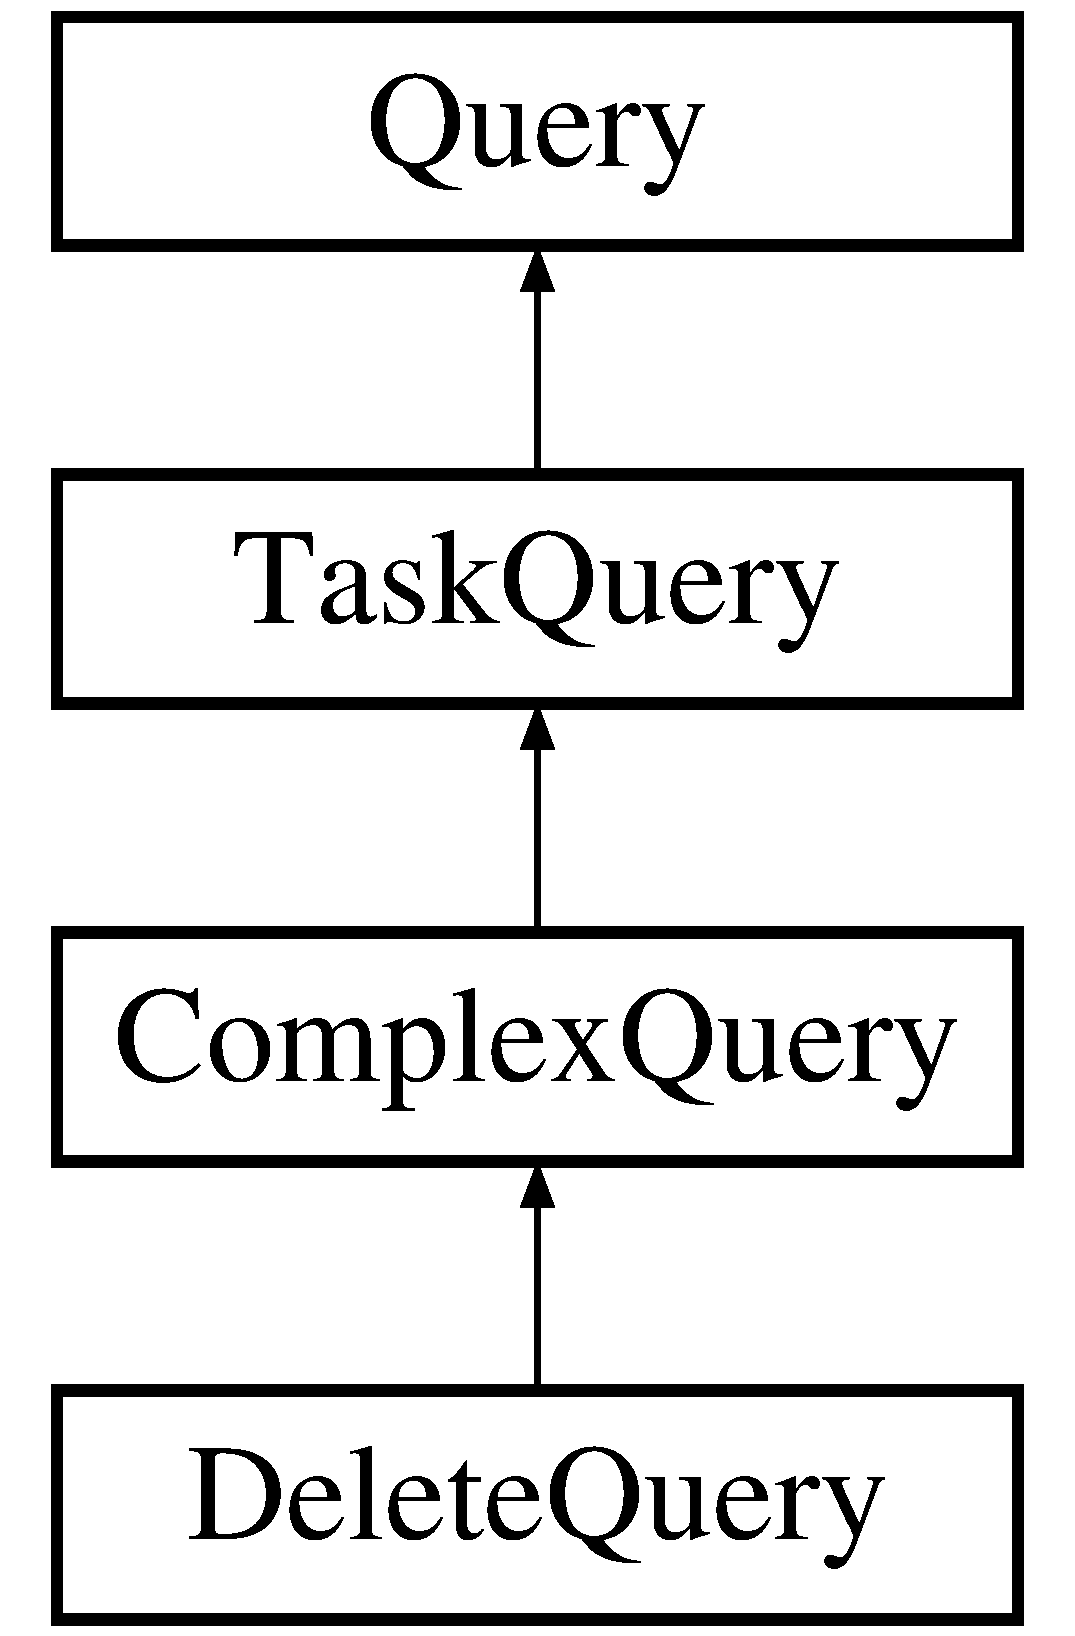
\includegraphics[height=4.000000cm]{class_delete_query}
\end{center}
\end{figure}
\subsection*{Public Member Functions}
\begin{DoxyCompactItemize}
\item 
\mbox{\Hypertarget{class_delete_query_aa95925b0055f7a3e502dd33914a9d091}\label{class_delete_query_aa95925b0055f7a3e502dd33914a9d091}} 
{\bfseries L\+E\+M\+O\+N\+D\+B\+\_\+\+Q\+U\+E\+R\+Y\+\_\+\+W\+R\+I\+T\+ER} (true)
\item 
\mbox{\Hypertarget{class_delete_query_a2f534f7366326b3aa84ee640f4072b98}\label{class_delete_query_a2f534f7366326b3aa84ee640f4072b98}} 
Query\+Result\+::\+Ptr {\bfseries execute} () override
\item 
\mbox{\Hypertarget{class_delete_query_a481620086e9d7560dbb6296876f6dcf1}\label{class_delete_query_a481620086e9d7560dbb6296876f6dcf1}} 
std\+::string {\bfseries to\+String} () override
\item 
\mbox{\Hypertarget{class_delete_query_ab36de51aead741d72069d1a95214c4cb}\label{class_delete_query_ab36de51aead741d72069d1a95214c4cb}} 
Query\+Result\+::\+Ptr {\bfseries combine} (int \hyperlink{class_task_query_a3dc3e4c56ddea8ff025239fd9da358d3}{task\+Complete}) override
\end{DoxyCompactItemize}
\subsection*{Friends}
\begin{DoxyCompactItemize}
\item 
\mbox{\Hypertarget{class_delete_query_ad20f61684a9dbe6fbec924694ed7068c}\label{class_delete_query_ad20f61684a9dbe6fbec924694ed7068c}} 
class {\bfseries Delete\+Task}
\end{DoxyCompactItemize}
\subsection*{Additional Inherited Members}


\subsection{Detailed Description}


Definition at line 11 of file delete\+\_\+query.\+h.



The documentation for this class was generated from the following files\+:\begin{DoxyCompactItemize}
\item 
src/query/data/delete\+\_\+query.\+h\item 
src/query/data/delete\+\_\+query.\+cpp\end{DoxyCompactItemize}

\hypertarget{class_delete_task}{}\section{Delete\+Task Class Reference}
\label{class_delete_task}\index{Delete\+Task@{Delete\+Task}}
Inheritance diagram for Delete\+Task\+:\begin{figure}[H]
\begin{center}
\leavevmode
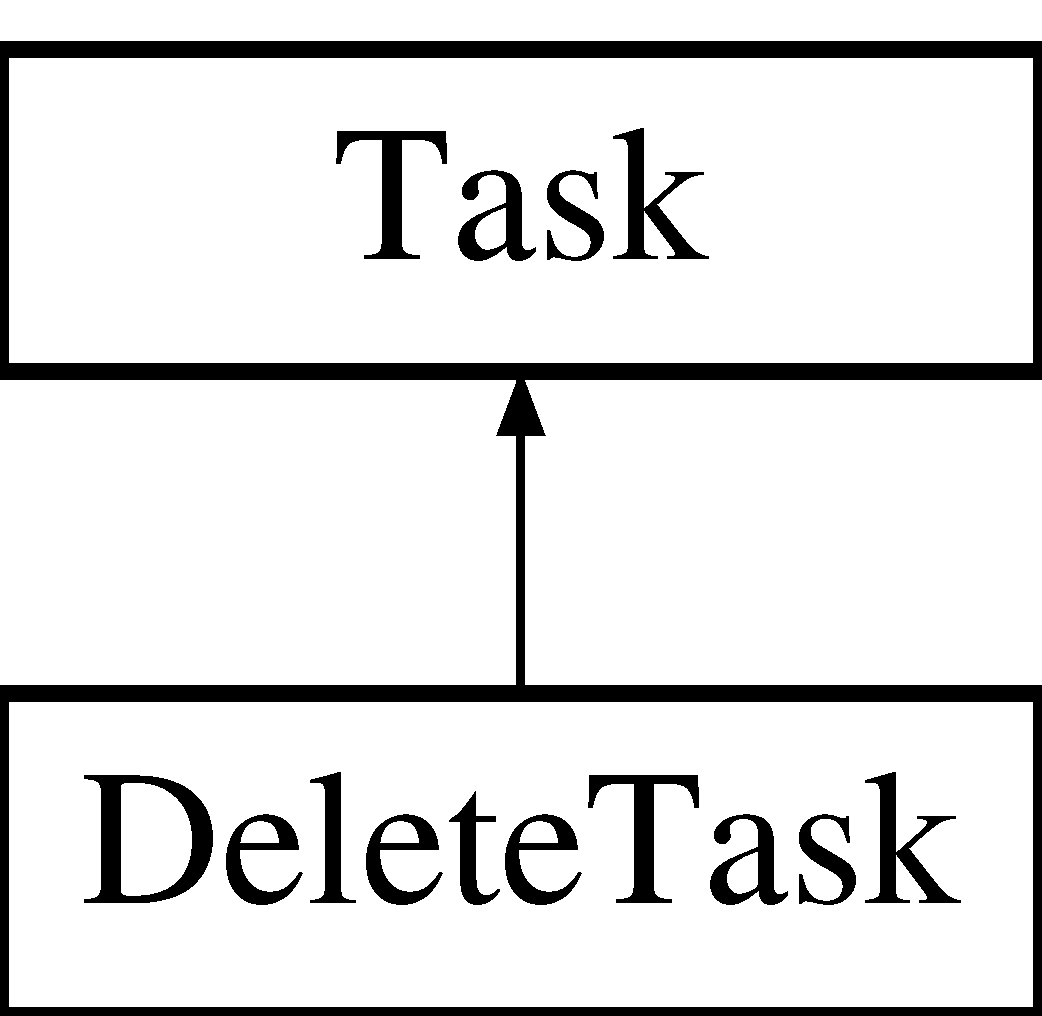
\includegraphics[height=2.000000cm]{class_delete_task}
\end{center}
\end{figure}
\subsection*{Public Member Functions}
\begin{DoxyCompactItemize}
\item 
\mbox{\Hypertarget{class_delete_task_a5f9ca85f1fcc0cb0fa8f88379aec97a3}\label{class_delete_task_a5f9ca85f1fcc0cb0fa8f88379aec97a3}} 
void {\bfseries execute} () override
\end{DoxyCompactItemize}
\subsection*{Protected Member Functions}
\begin{DoxyCompactItemize}
\item 
\mbox{\Hypertarget{class_delete_task_ad01f73fd1fc4af6261d78ff70e6b5e76}\label{class_delete_task_ad01f73fd1fc4af6261d78ff70e6b5e76}} 
{\bfseries L\+E\+M\+O\+N\+D\+B\+\_\+\+Q\+U\+E\+R\+Y\+\_\+\+P\+TR} (\hyperlink{class_delete_query}{Delete\+Query})
\end{DoxyCompactItemize}
\subsection*{Additional Inherited Members}


\subsection{Detailed Description}


Definition at line 22 of file delete\+\_\+query.\+h.



The documentation for this class was generated from the following files\+:\begin{DoxyCompactItemize}
\item 
src/query/data/delete\+\_\+query.\+h\item 
src/query/data/delete\+\_\+query.\+cpp\end{DoxyCompactItemize}

\hypertarget{class_drop_table_query}{}\section{Drop\+Table\+Query Class Reference}
\label{class_drop_table_query}\index{Drop\+Table\+Query@{Drop\+Table\+Query}}
Inheritance diagram for Drop\+Table\+Query\+:\begin{figure}[H]
\begin{center}
\leavevmode
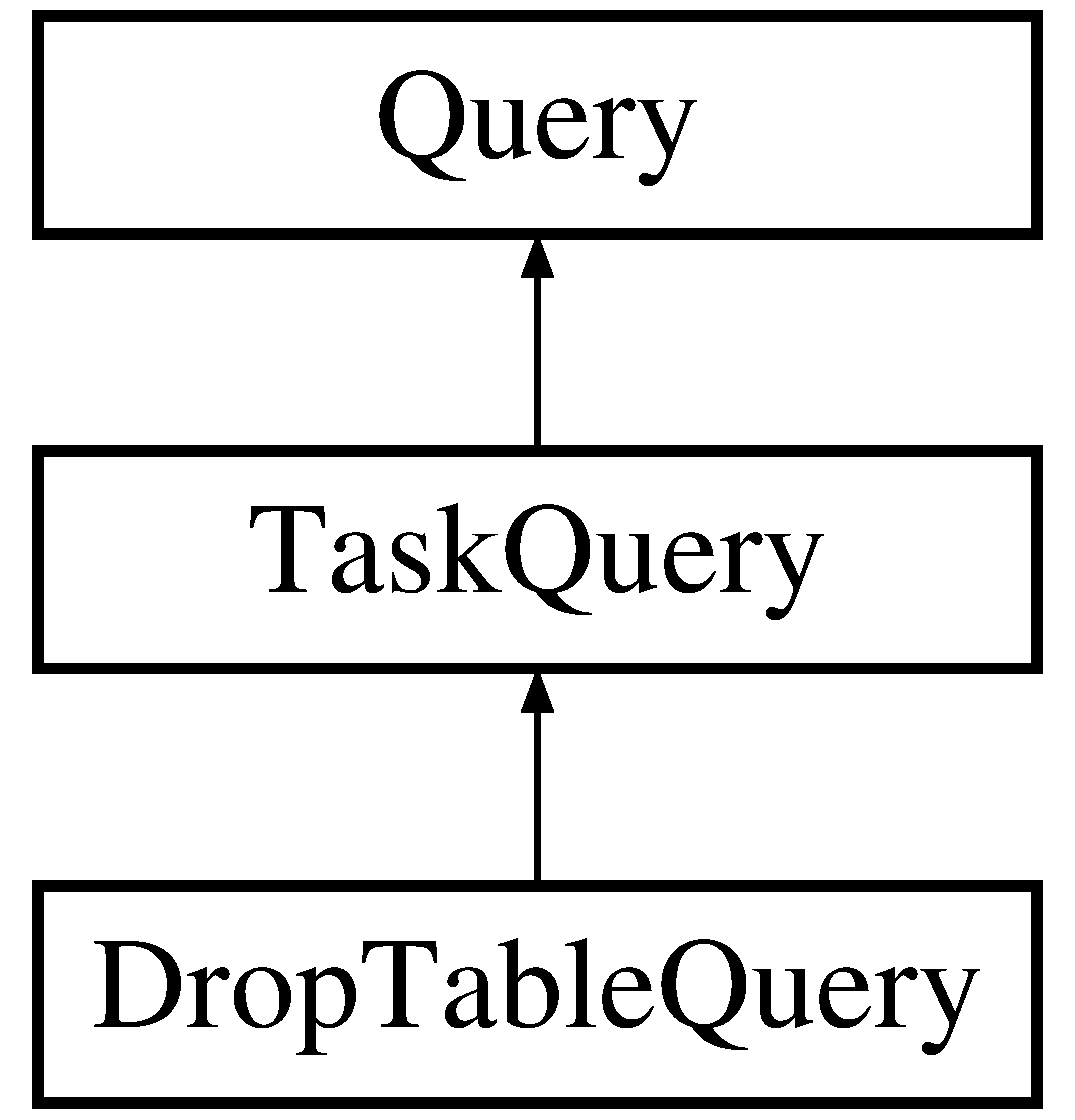
\includegraphics[height=3.000000cm]{class_drop_table_query}
\end{center}
\end{figure}
\subsection*{Public Member Functions}
\begin{DoxyCompactItemize}
\item 
\mbox{\Hypertarget{class_drop_table_query_a09612e6e0f58bc03fa664a67fe92be8f}\label{class_drop_table_query_a09612e6e0f58bc03fa664a67fe92be8f}} 
Query\+Result\+::\+Ptr {\bfseries execute} () override
\item 
\mbox{\Hypertarget{class_drop_table_query_a30eb39edc286cdd15bed4fc791f76d38}\label{class_drop_table_query_a30eb39edc286cdd15bed4fc791f76d38}} 
std\+::string {\bfseries to\+String} () override
\end{DoxyCompactItemize}
\subsection*{Additional Inherited Members}


\subsection{Detailed Description}


Definition at line 11 of file drop\+\_\+query.\+h.



The documentation for this class was generated from the following files\+:\begin{DoxyCompactItemize}
\item 
src/query/management/drop\+\_\+query.\+h\item 
src/query/management/drop\+\_\+query.\+cpp\end{DoxyCompactItemize}

\hypertarget{class_dump_table_query}{}\section{Dump\+Table\+Query Class Reference}
\label{class_dump_table_query}\index{Dump\+Table\+Query@{Dump\+Table\+Query}}
Inheritance diagram for Dump\+Table\+Query\+:\begin{figure}[H]
\begin{center}
\leavevmode
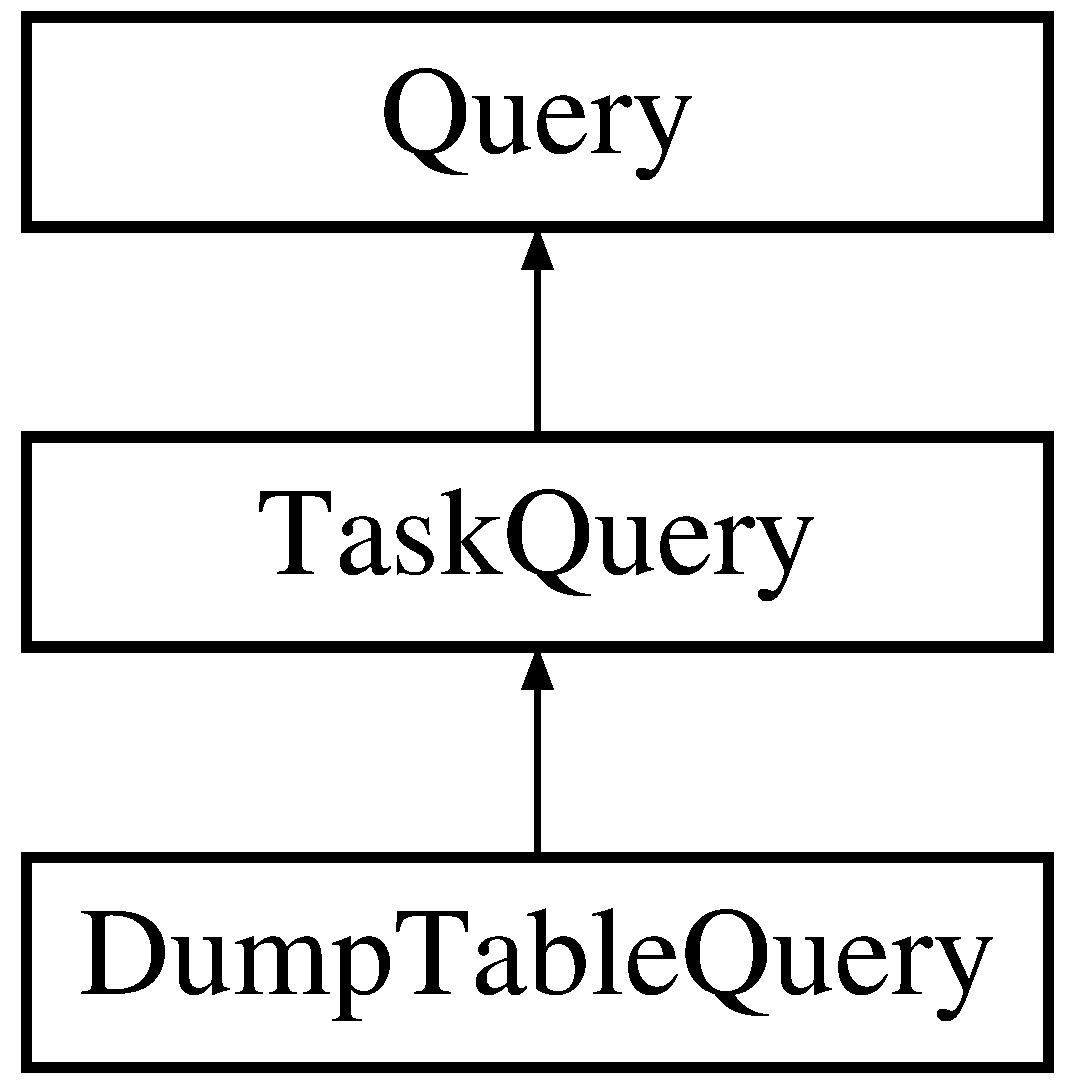
\includegraphics[height=3.000000cm]{class_dump_table_query}
\end{center}
\end{figure}
\subsection*{Public Member Functions}
\begin{DoxyCompactItemize}
\item 
\mbox{\Hypertarget{class_dump_table_query_a0d5ee4ef52e21cbc7cb87bc4153ce43a}\label{class_dump_table_query_a0d5ee4ef52e21cbc7cb87bc4153ce43a}} 
{\bfseries Dump\+Table\+Query} (std\+::string table, std\+::string filename)
\item 
\mbox{\Hypertarget{class_dump_table_query_a6717d017981e962930a0951b3c519f68}\label{class_dump_table_query_a6717d017981e962930a0951b3c519f68}} 
Query\+Result\+::\+Ptr {\bfseries execute} () override
\item 
\mbox{\Hypertarget{class_dump_table_query_a4047a2abe9bd6322c9a68bf1c4fb1476}\label{class_dump_table_query_a4047a2abe9bd6322c9a68bf1c4fb1476}} 
std\+::string {\bfseries to\+String} () override
\item 
\mbox{\Hypertarget{class_dump_table_query_a0e379595f545ff2cc2fed17763bf0f86}\label{class_dump_table_query_a0e379595f545ff2cc2fed17763bf0f86}} 
Query\+Result\+::\+Ptr {\bfseries combine} (int \hyperlink{class_task_query_a3dc3e4c56ddea8ff025239fd9da358d3}{task\+Complete}) override
\end{DoxyCompactItemize}
\subsection*{Friends}
\begin{DoxyCompactItemize}
\item 
\mbox{\Hypertarget{class_dump_table_query_a790c02b26168b984552211bd81cf2305}\label{class_dump_table_query_a790c02b26168b984552211bd81cf2305}} 
class {\bfseries Dump\+Table\+Task}
\end{DoxyCompactItemize}
\subsection*{Additional Inherited Members}


\subsection{Detailed Description}


Definition at line 11 of file dump\+\_\+query.\+h.



The documentation for this class was generated from the following files\+:\begin{DoxyCompactItemize}
\item 
src/query/management/dump\+\_\+query.\+h\item 
src/query/management/dump\+\_\+query.\+cpp\end{DoxyCompactItemize}

\hypertarget{class_dump_table_task}{}\section{Dump\+Table\+Task Class Reference}
\label{class_dump_table_task}\index{Dump\+Table\+Task@{Dump\+Table\+Task}}
Inheritance diagram for Dump\+Table\+Task\+:\begin{figure}[H]
\begin{center}
\leavevmode
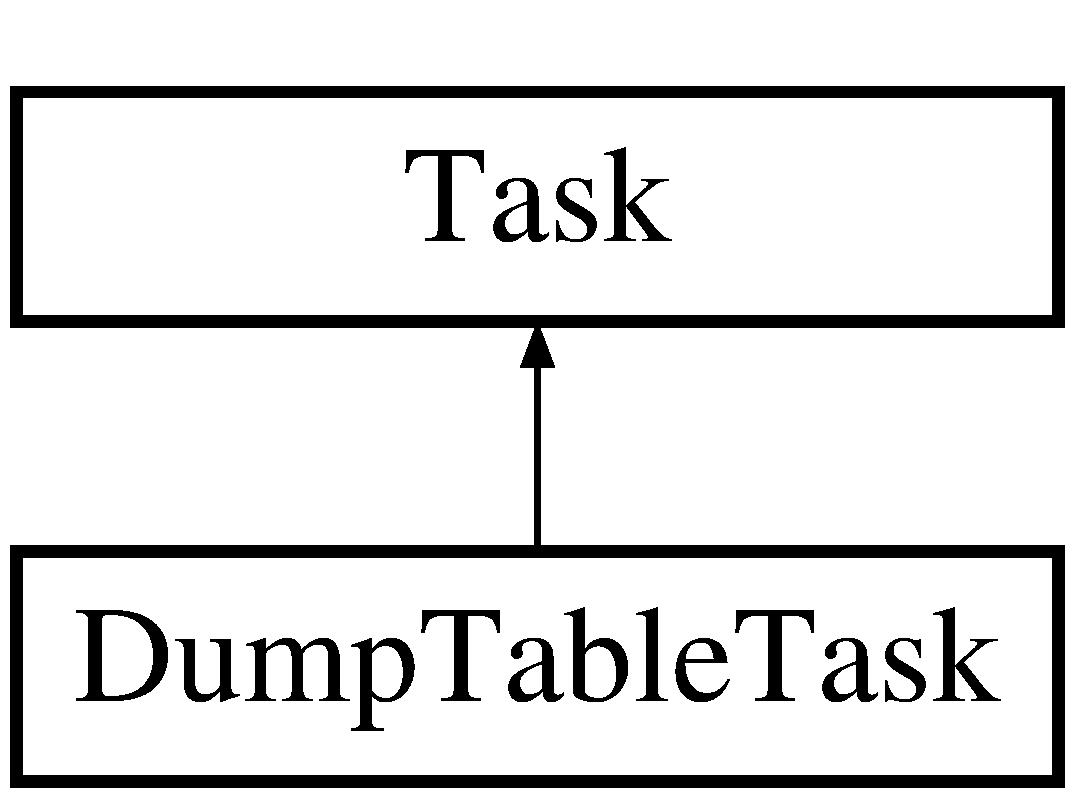
\includegraphics[height=2.000000cm]{class_dump_table_task}
\end{center}
\end{figure}
\subsection*{Public Member Functions}
\begin{DoxyCompactItemize}
\item 
\mbox{\Hypertarget{class_dump_table_task_a5beb6d0ee8d22ac6580077f0233b512c}\label{class_dump_table_task_a5beb6d0ee8d22ac6580077f0233b512c}} 
void {\bfseries execute} () override
\end{DoxyCompactItemize}
\subsection*{Protected Member Functions}
\begin{DoxyCompactItemize}
\item 
\mbox{\Hypertarget{class_dump_table_task_abc06bc4e6393ed9cf1391ecb3c47af33}\label{class_dump_table_task_abc06bc4e6393ed9cf1391ecb3c47af33}} 
{\bfseries L\+E\+M\+O\+N\+D\+B\+\_\+\+Q\+U\+E\+R\+Y\+\_\+\+P\+TR} (\hyperlink{class_dump_table_query}{Dump\+Table\+Query})
\end{DoxyCompactItemize}
\subsection*{Additional Inherited Members}


\subsection{Detailed Description}


Definition at line 24 of file dump\+\_\+query.\+h.



The documentation for this class was generated from the following files\+:\begin{DoxyCompactItemize}
\item 
src/query/management/dump\+\_\+query.\+h\item 
src/query/management/dump\+\_\+query.\+cpp\end{DoxyCompactItemize}

\hypertarget{struct_duplicated_table_name}{}\section{Duplicated\+Table\+Name Struct Reference}
\label{struct_duplicated_table_name}\index{Duplicated\+Table\+Name@{Duplicated\+Table\+Name}}
Inheritance diagram for Duplicated\+Table\+Name\+:\begin{figure}[H]
\begin{center}
\leavevmode
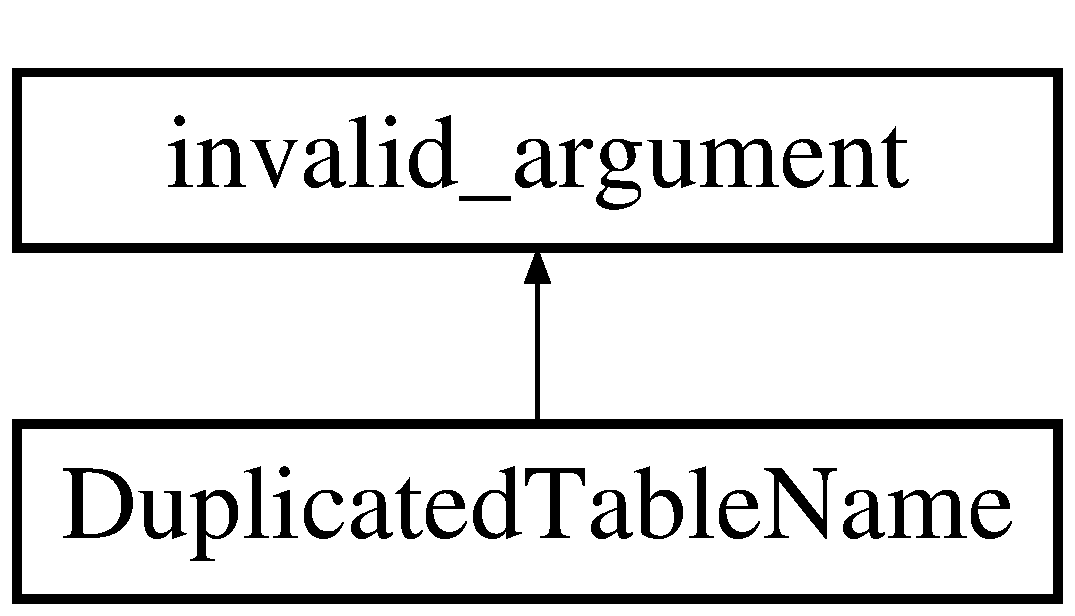
\includegraphics[height=2.000000cm]{struct_duplicated_table_name}
\end{center}
\end{figure}
\subsection*{Public Member Functions}
\begin{DoxyCompactItemize}
\item 
\mbox{\Hypertarget{struct_duplicated_table_name_ae19eda8ab536d93718c7d471a50d48b6}\label{struct_duplicated_table_name_ae19eda8ab536d93718c7d471a50d48b6}} 
{\bfseries Duplicated\+Table\+Name} (const std\+::string \&str)
\end{DoxyCompactItemize}


\subsection{Detailed Description}


Definition at line 16 of file uexception.\+h.



The documentation for this struct was generated from the following file\+:\begin{DoxyCompactItemize}
\item 
src/uexception.\+h\end{DoxyCompactItemize}

\hypertarget{class_duplicate_query}{}\section{Duplicate\+Query Class Reference}
\label{class_duplicate_query}\index{Duplicate\+Query@{Duplicate\+Query}}
Inheritance diagram for Duplicate\+Query\+:\begin{figure}[H]
\begin{center}
\leavevmode
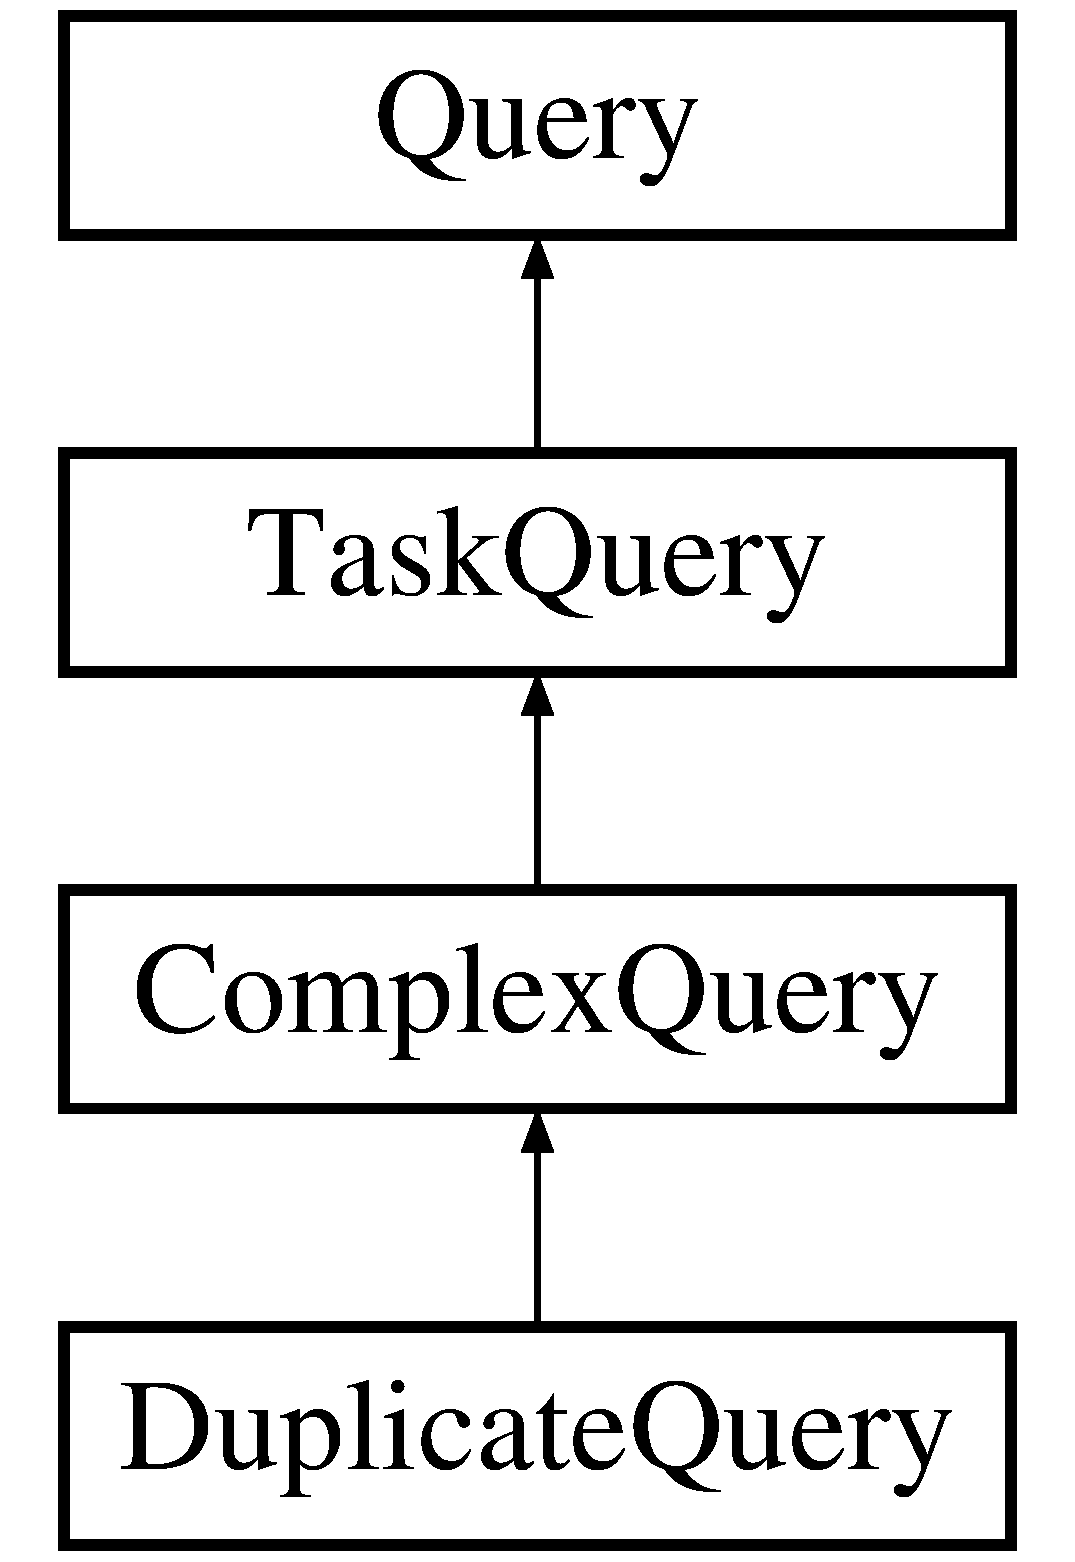
\includegraphics[height=4.000000cm]{class_duplicate_query}
\end{center}
\end{figure}
\subsection*{Public Member Functions}
\begin{DoxyCompactItemize}
\item 
\mbox{\Hypertarget{class_duplicate_query_ae7356ed3cbffe8ee72ede6a05c542686}\label{class_duplicate_query_ae7356ed3cbffe8ee72ede6a05c542686}} 
{\bfseries L\+E\+M\+O\+N\+D\+B\+\_\+\+Q\+U\+E\+R\+Y\+\_\+\+W\+R\+I\+T\+ER} (true)
\item 
\mbox{\Hypertarget{class_duplicate_query_ab7ce5d0d57cc839ff330de7e016354b0}\label{class_duplicate_query_ab7ce5d0d57cc839ff330de7e016354b0}} 
Query\+Result\+::\+Ptr {\bfseries execute} () override
\item 
\mbox{\Hypertarget{class_duplicate_query_af1f379a04b6eb6940e97fe4c33d171a7}\label{class_duplicate_query_af1f379a04b6eb6940e97fe4c33d171a7}} 
std\+::string {\bfseries to\+String} () override
\item 
\mbox{\Hypertarget{class_duplicate_query_ae3b387fdae8793a92020f2946b6c0086}\label{class_duplicate_query_ae3b387fdae8793a92020f2946b6c0086}} 
Query\+Result\+::\+Ptr {\bfseries combine} (int \hyperlink{class_task_query_a3dc3e4c56ddea8ff025239fd9da358d3}{task\+Complete}) override
\end{DoxyCompactItemize}
\subsection*{Friends}
\begin{DoxyCompactItemize}
\item 
\mbox{\Hypertarget{class_duplicate_query_ac4a27d08853bb2e571fb2d74a3b9be3b}\label{class_duplicate_query_ac4a27d08853bb2e571fb2d74a3b9be3b}} 
class {\bfseries Duplicate\+Task}
\end{DoxyCompactItemize}
\subsection*{Additional Inherited Members}


\subsection{Detailed Description}


Definition at line 11 of file duplicate\+\_\+query.\+h.



The documentation for this class was generated from the following files\+:\begin{DoxyCompactItemize}
\item 
src/query/data/duplicate\+\_\+query.\+h\item 
src/query/data/duplicate\+\_\+query.\+cpp\end{DoxyCompactItemize}

\hypertarget{class_duplicate_task}{}\section{Duplicate\+Task Class Reference}
\label{class_duplicate_task}\index{Duplicate\+Task@{Duplicate\+Task}}
Inheritance diagram for Duplicate\+Task\+:\begin{figure}[H]
\begin{center}
\leavevmode
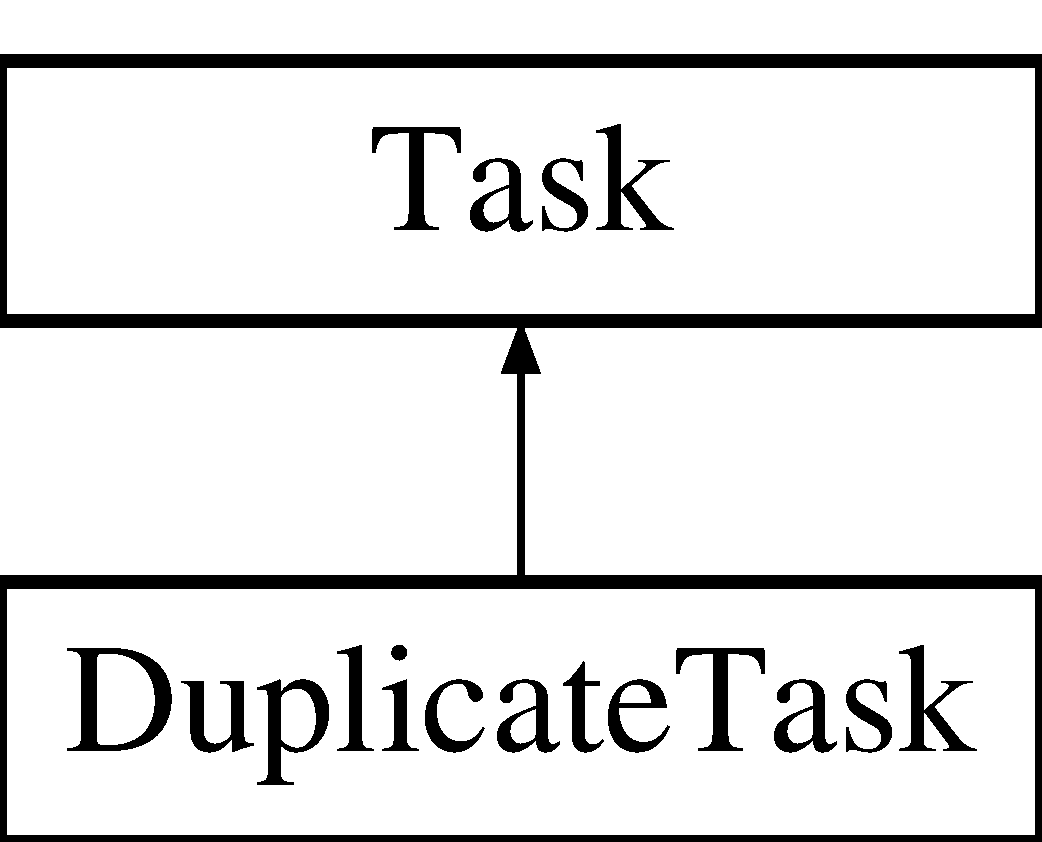
\includegraphics[height=2.000000cm]{class_duplicate_task}
\end{center}
\end{figure}
\subsection*{Public Member Functions}
\begin{DoxyCompactItemize}
\item 
\mbox{\Hypertarget{class_duplicate_task_a0163417206331d992839f28b8090b87c}\label{class_duplicate_task_a0163417206331d992839f28b8090b87c}} 
void {\bfseries execute} () override
\end{DoxyCompactItemize}
\subsection*{Protected Member Functions}
\begin{DoxyCompactItemize}
\item 
\mbox{\Hypertarget{class_duplicate_task_a1dcec62cac0f05d33eb4bbd261889380}\label{class_duplicate_task_a1dcec62cac0f05d33eb4bbd261889380}} 
{\bfseries L\+E\+M\+O\+N\+D\+B\+\_\+\+Q\+U\+E\+R\+Y\+\_\+\+P\+TR} (\hyperlink{class_duplicate_query}{Duplicate\+Query})
\end{DoxyCompactItemize}
\subsection*{Additional Inherited Members}


\subsection{Detailed Description}


Definition at line 22 of file duplicate\+\_\+query.\+h.



The documentation for this class was generated from the following files\+:\begin{DoxyCompactItemize}
\item 
src/query/data/duplicate\+\_\+query.\+h\item 
src/query/data/duplicate\+\_\+query.\+cpp\end{DoxyCompactItemize}

\hypertarget{class_error_msg_result}{}\section{Error\+Msg\+Result Class Reference}
\label{class_error_msg_result}\index{Error\+Msg\+Result@{Error\+Msg\+Result}}
Inheritance diagram for Error\+Msg\+Result\+:\begin{figure}[H]
\begin{center}
\leavevmode
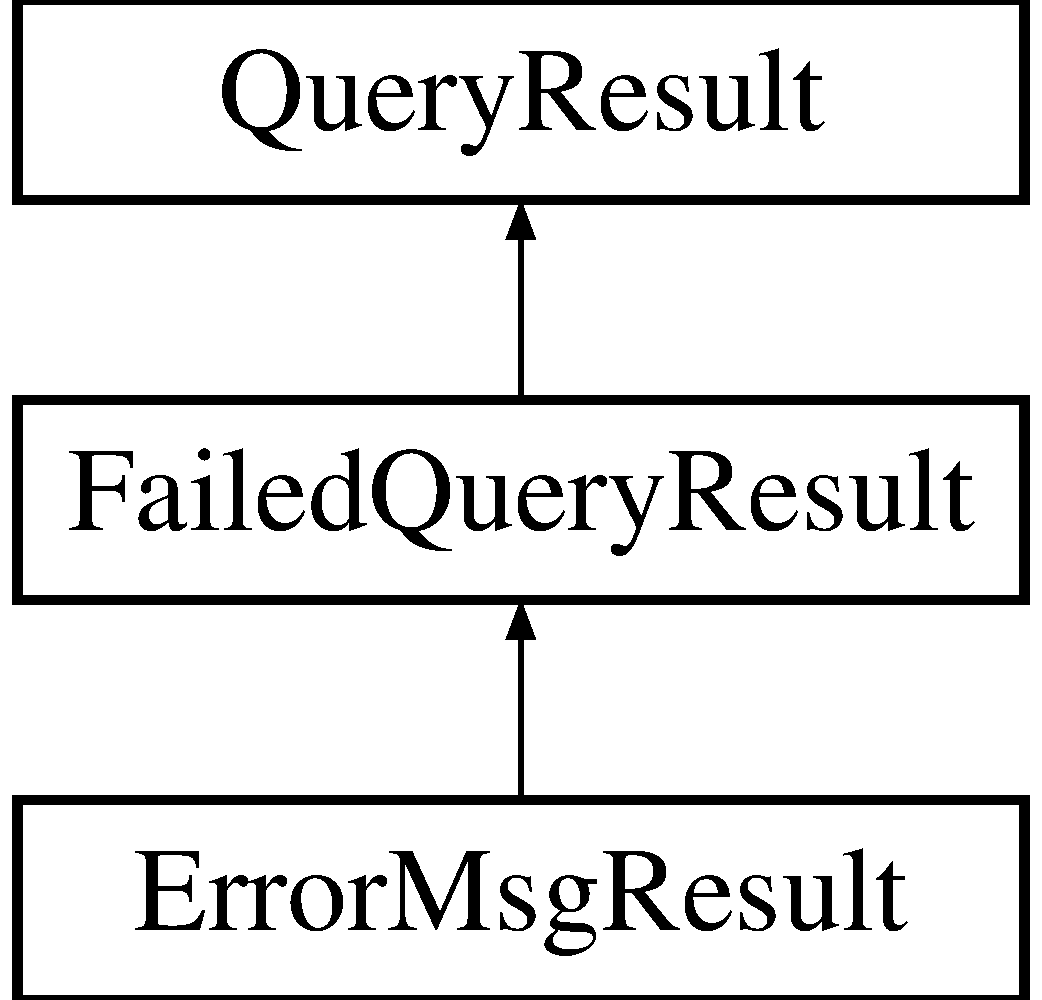
\includegraphics[height=3.000000cm]{class_error_msg_result}
\end{center}
\end{figure}
\subsection*{Public Member Functions}
\begin{DoxyCompactItemize}
\item 
\mbox{\Hypertarget{class_error_msg_result_a29e5dbbffb8b5f0bd62d00426fe3eb4b}\label{class_error_msg_result_a29e5dbbffb8b5f0bd62d00426fe3eb4b}} 
{\bfseries Error\+Msg\+Result} (const char $\ast$qname, const std\+::string \&msg)
\item 
\mbox{\Hypertarget{class_error_msg_result_aa45c38fbcbc8e893a96221938d3d4d32}\label{class_error_msg_result_aa45c38fbcbc8e893a96221938d3d4d32}} 
{\bfseries Error\+Msg\+Result} (const char $\ast$qname, const char $\ast$table, const std\+::string \&msg)
\item 
\mbox{\Hypertarget{class_error_msg_result_a6cf0d89a560e0857bbb95a702e0fbfc8}\label{class_error_msg_result_a6cf0d89a560e0857bbb95a702e0fbfc8}} 
std\+::string {\bfseries to\+String} () override
\end{DoxyCompactItemize}
\subsection*{Additional Inherited Members}


\subsection{Detailed Description}


Definition at line 40 of file query\+\_\+results.\+h.



The documentation for this class was generated from the following file\+:\begin{DoxyCompactItemize}
\item 
src/query\+\_\+results.\+h\end{DoxyCompactItemize}

\hypertarget{class_failed_query_builder}{}\section{Failed\+Query\+Builder Class Reference}
\label{class_failed_query_builder}\index{Failed\+Query\+Builder@{Failed\+Query\+Builder}}
Inheritance diagram for Failed\+Query\+Builder\+:\begin{figure}[H]
\begin{center}
\leavevmode
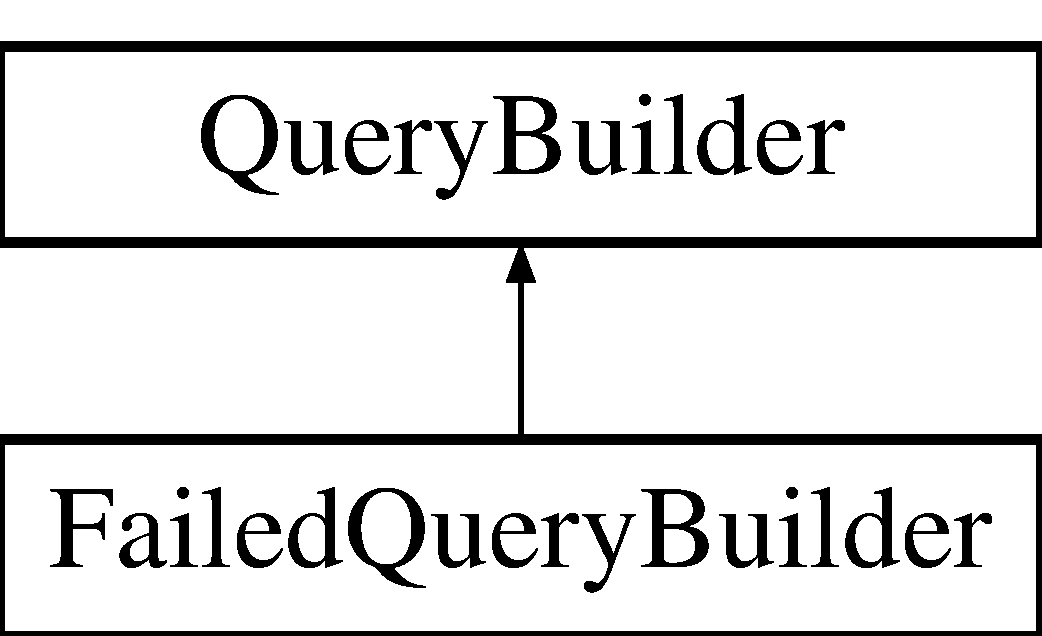
\includegraphics[height=2.000000cm]{class_failed_query_builder}
\end{center}
\end{figure}
\subsection*{Public Member Functions}
\begin{DoxyCompactItemize}
\item 
\mbox{\Hypertarget{class_failed_query_builder_a3f6d775ce553c92eb1c12fe87e90f60e}\label{class_failed_query_builder_a3f6d775ce553c92eb1c12fe87e90f60e}} 
Query\+::\+Ptr {\bfseries try\+Extract\+Query} (\hyperlink{struct_tokenized_query_string}{Tokenized\+Query\+String} \&q) final
\item 
\mbox{\Hypertarget{class_failed_query_builder_add3120fe7949f737a6c833db1dcd34d8}\label{class_failed_query_builder_add3120fe7949f737a6c833db1dcd34d8}} 
void {\bfseries set\+Next} (Query\+Builder\+::\+Ptr \&\&builder) final
\item 
\mbox{\Hypertarget{class_failed_query_builder_acfb81aa5e49f10869aca93a47d175c23}\label{class_failed_query_builder_acfb81aa5e49f10869aca93a47d175c23}} 
void {\bfseries clear} () override
\end{DoxyCompactItemize}
\subsection*{Static Public Member Functions}
\begin{DoxyCompactItemize}
\item 
\mbox{\Hypertarget{class_failed_query_builder_a8f37cc4b7fd48f5c6ee47063ea6faa00}\label{class_failed_query_builder_a8f37cc4b7fd48f5c6ee47063ea6faa00}} 
static Query\+Builder\+::\+Ptr {\bfseries get\+Default} ()
\end{DoxyCompactItemize}
\subsection*{Additional Inherited Members}


\subsection{Detailed Description}


Definition at line 24 of file query\+\_\+builders.\+h.



The documentation for this class was generated from the following file\+:\begin{DoxyCompactItemize}
\item 
src/query\+\_\+builders.\+h\end{DoxyCompactItemize}

\hypertarget{class_failed_query_result}{}\section{Failed\+Query\+Result Class Reference}
\label{class_failed_query_result}\index{Failed\+Query\+Result@{Failed\+Query\+Result}}
Inheritance diagram for Failed\+Query\+Result\+:\begin{figure}[H]
\begin{center}
\leavevmode
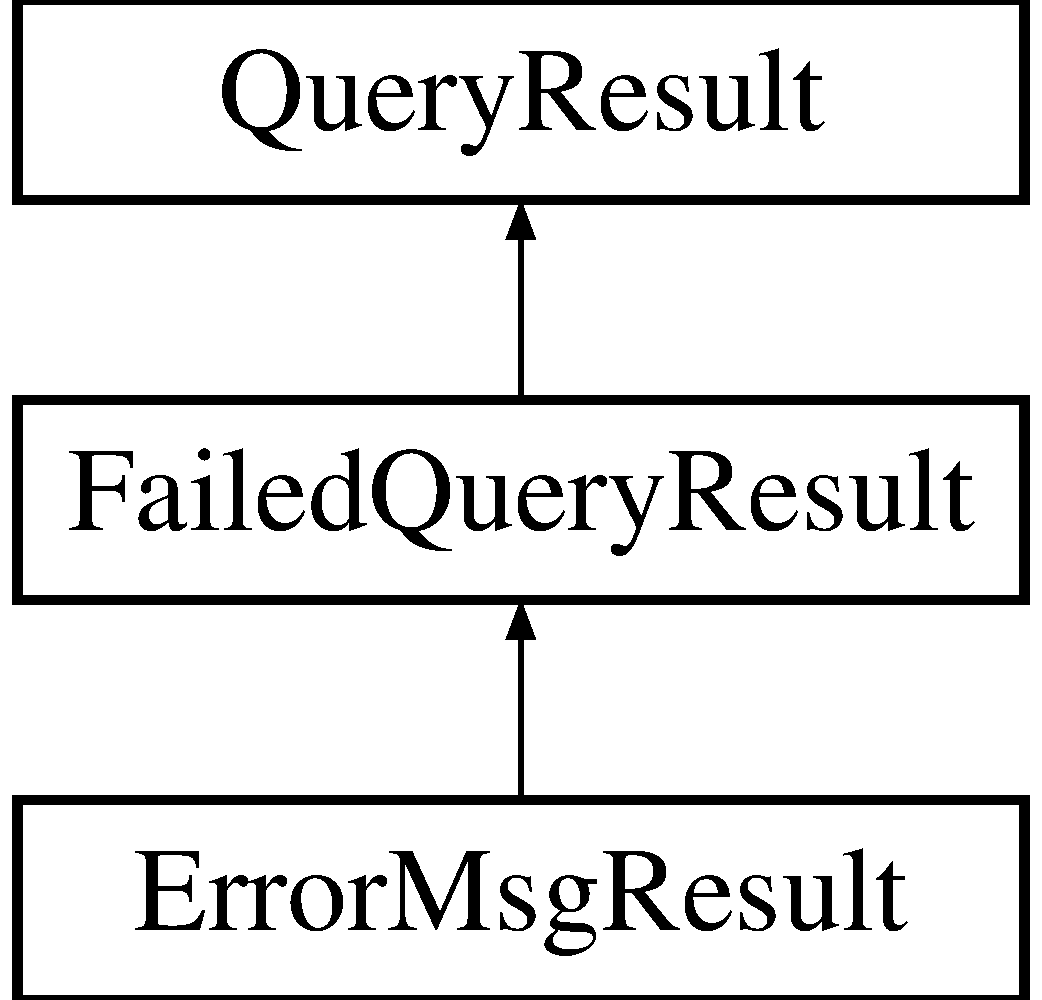
\includegraphics[height=3.000000cm]{class_failed_query_result}
\end{center}
\end{figure}
\subsection*{Public Member Functions}
\begin{DoxyCompactItemize}
\item 
\mbox{\Hypertarget{class_failed_query_result_a4e742c22aa57a13cca1cfb3b3b05f63d}\label{class_failed_query_result_a4e742c22aa57a13cca1cfb3b3b05f63d}} 
bool {\bfseries success} () override
\end{DoxyCompactItemize}
\subsection*{Additional Inherited Members}


\subsection{Detailed Description}


Definition at line 22 of file query\+\_\+results.\+h.



The documentation for this class was generated from the following file\+:\begin{DoxyCompactItemize}
\item 
src/query\+\_\+results.\+h\end{DoxyCompactItemize}

\hypertarget{struct_ill_formed_query}{}\section{Ill\+Formed\+Query Struct Reference}
\label{struct_ill_formed_query}\index{Ill\+Formed\+Query@{Ill\+Formed\+Query}}
Inheritance diagram for Ill\+Formed\+Query\+:\begin{figure}[H]
\begin{center}
\leavevmode
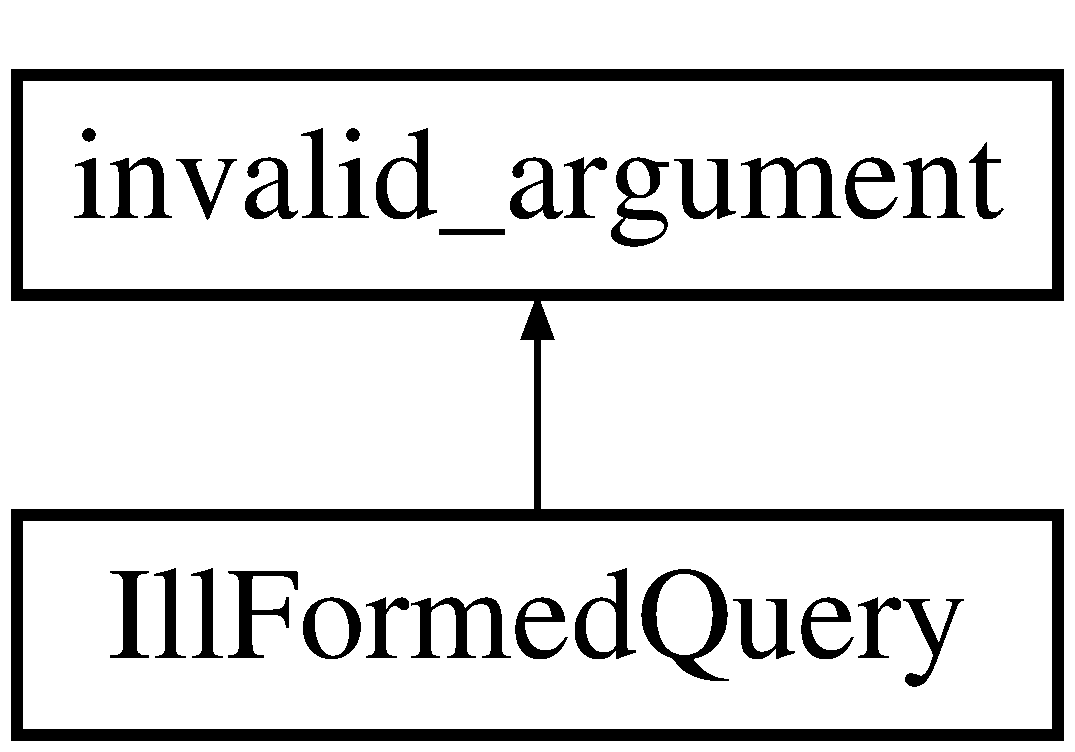
\includegraphics[height=2.000000cm]{struct_ill_formed_query}
\end{center}
\end{figure}
\subsection*{Public Member Functions}
\begin{DoxyCompactItemize}
\item 
\mbox{\Hypertarget{struct_ill_formed_query_a1c561f3dcf8ff9592e9a00f9bff5ee11}\label{struct_ill_formed_query_a1c561f3dcf8ff9592e9a00f9bff5ee11}} 
{\bfseries Ill\+Formed\+Query} (const std\+::string \&str)
\end{DoxyCompactItemize}


\subsection{Detailed Description}


Definition at line 46 of file uexception.\+h.



The documentation for this struct was generated from the following file\+:\begin{DoxyCompactItemize}
\item 
src/uexception.\+h\end{DoxyCompactItemize}

\hypertarget{struct_ill_formed_query_condition}{}\section{Ill\+Formed\+Query\+Condition Struct Reference}
\label{struct_ill_formed_query_condition}\index{Ill\+Formed\+Query\+Condition@{Ill\+Formed\+Query\+Condition}}
Inheritance diagram for Ill\+Formed\+Query\+Condition\+:\begin{figure}[H]
\begin{center}
\leavevmode
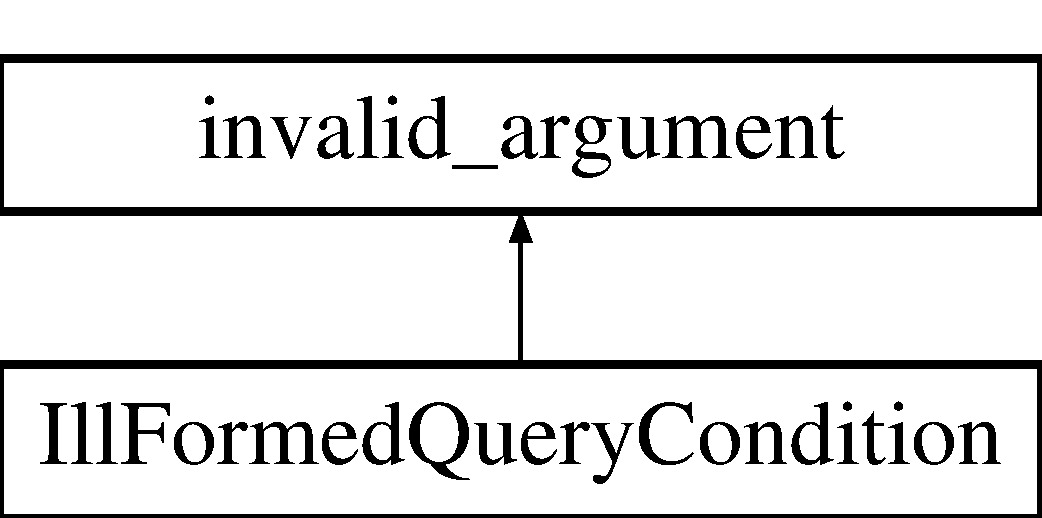
\includegraphics[height=2.000000cm]{struct_ill_formed_query_condition}
\end{center}
\end{figure}
\subsection*{Public Member Functions}
\begin{DoxyCompactItemize}
\item 
\mbox{\Hypertarget{struct_ill_formed_query_condition_a05ad150e00ad1cf9f9f33f78c9f1b2f9}\label{struct_ill_formed_query_condition_a05ad150e00ad1cf9f9f33f78c9f1b2f9}} 
{\bfseries Ill\+Formed\+Query\+Condition} (const std\+::string \&str)
\end{DoxyCompactItemize}


\subsection{Detailed Description}


Definition at line 51 of file uexception.\+h.



The documentation for this struct was generated from the following file\+:\begin{DoxyCompactItemize}
\item 
src/uexception.\+h\end{DoxyCompactItemize}

\hypertarget{class_insert_query}{}\section{Insert\+Query Class Reference}
\label{class_insert_query}\index{Insert\+Query@{Insert\+Query}}
Inheritance diagram for Insert\+Query\+:\begin{figure}[H]
\begin{center}
\leavevmode
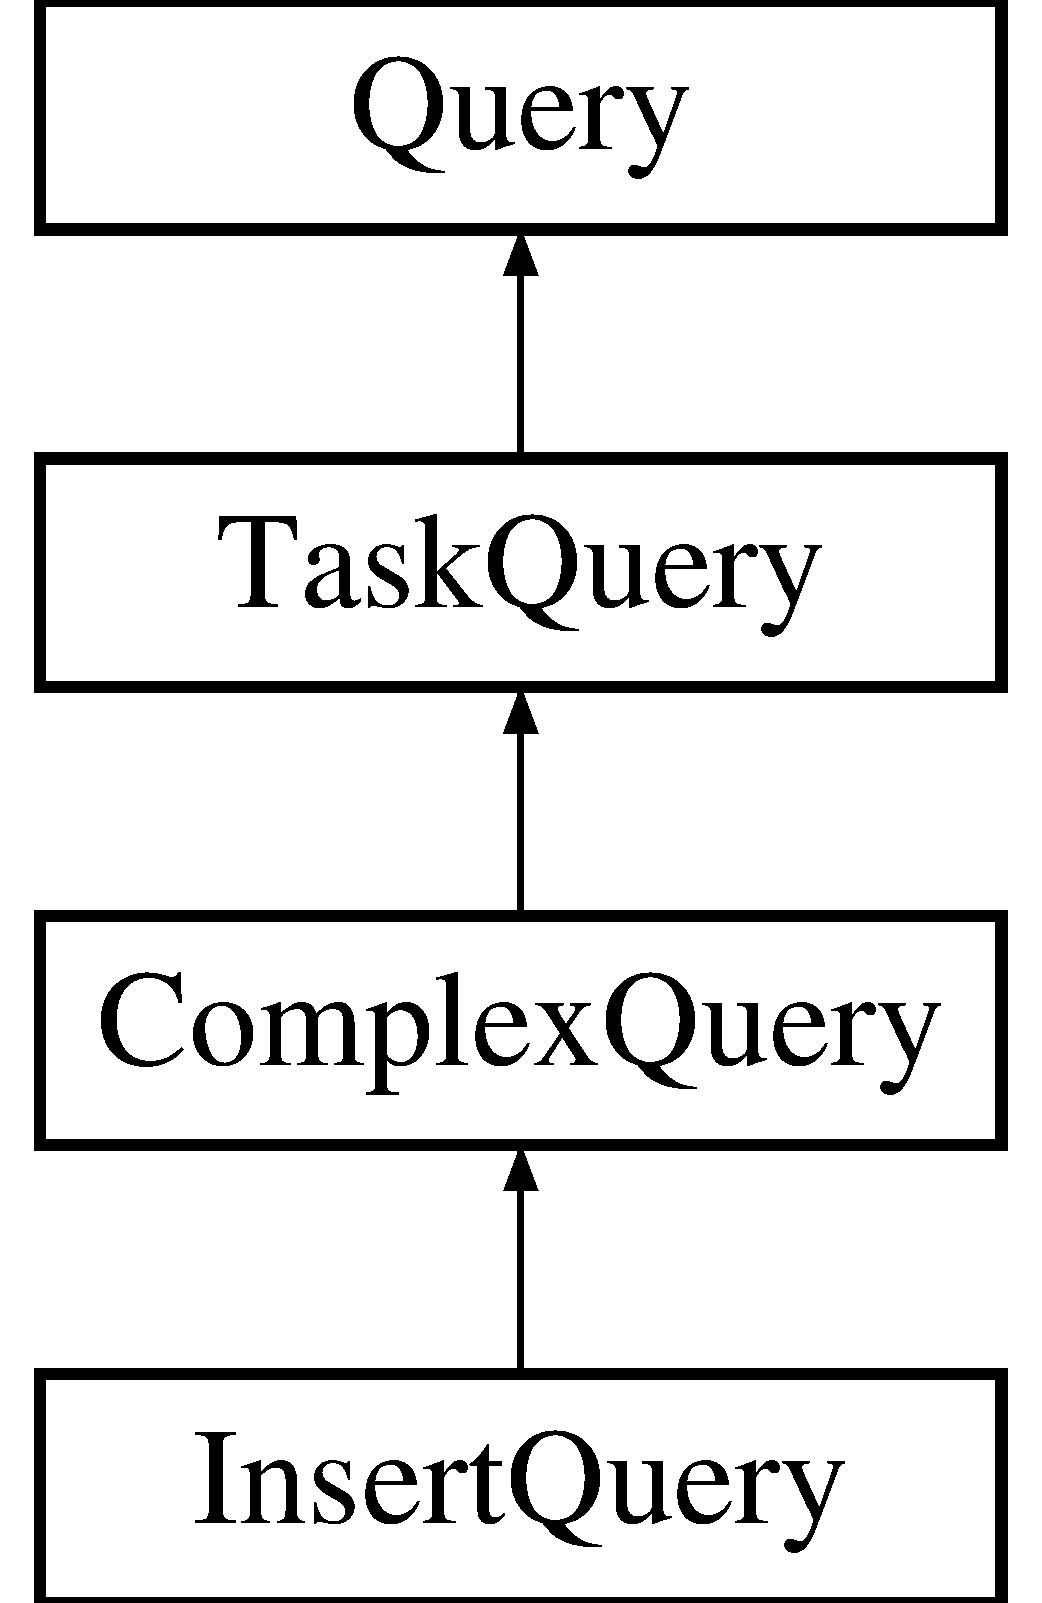
\includegraphics[height=4.000000cm]{class_insert_query}
\end{center}
\end{figure}
\subsection*{Public Member Functions}
\begin{DoxyCompactItemize}
\item 
\mbox{\Hypertarget{class_insert_query_a7f00e4f5ba3c1176c246095279768d84}\label{class_insert_query_a7f00e4f5ba3c1176c246095279768d84}} 
{\bfseries L\+E\+M\+O\+N\+D\+B\+\_\+\+Q\+U\+E\+R\+Y\+\_\+\+W\+R\+I\+T\+ER} (true)
\item 
\mbox{\Hypertarget{class_insert_query_acc4b700893c1c317db7a347d82ab548d}\label{class_insert_query_acc4b700893c1c317db7a347d82ab548d}} 
Query\+Result\+::\+Ptr {\bfseries execute} () override
\item 
\mbox{\Hypertarget{class_insert_query_aab9bd4260dbc60e073e7ca7d875d8dd8}\label{class_insert_query_aab9bd4260dbc60e073e7ca7d875d8dd8}} 
std\+::string {\bfseries to\+String} () override
\item 
\mbox{\Hypertarget{class_insert_query_a4cdcd69fce64e1910eef37ffe802a86d}\label{class_insert_query_a4cdcd69fce64e1910eef37ffe802a86d}} 
Query\+Result\+::\+Ptr {\bfseries combine} (int \hyperlink{class_task_query_a3dc3e4c56ddea8ff025239fd9da358d3}{task\+Complete}) override
\end{DoxyCompactItemize}
\subsection*{Friends}
\begin{DoxyCompactItemize}
\item 
\mbox{\Hypertarget{class_insert_query_a046ec31f5d7d865cd0cbe8b34cd2a108}\label{class_insert_query_a046ec31f5d7d865cd0cbe8b34cd2a108}} 
class {\bfseries Insert\+Task}
\end{DoxyCompactItemize}
\subsection*{Additional Inherited Members}


\subsection{Detailed Description}


Definition at line 7 of file insert\+\_\+query.\+h.



The documentation for this class was generated from the following files\+:\begin{DoxyCompactItemize}
\item 
src/query/data/insert\+\_\+query.\+h\item 
src/query/data/insert\+\_\+query.\+cpp\end{DoxyCompactItemize}

\hypertarget{class_insert_task}{}\section{Insert\+Task Class Reference}
\label{class_insert_task}\index{Insert\+Task@{Insert\+Task}}
Inheritance diagram for Insert\+Task\+:\begin{figure}[H]
\begin{center}
\leavevmode
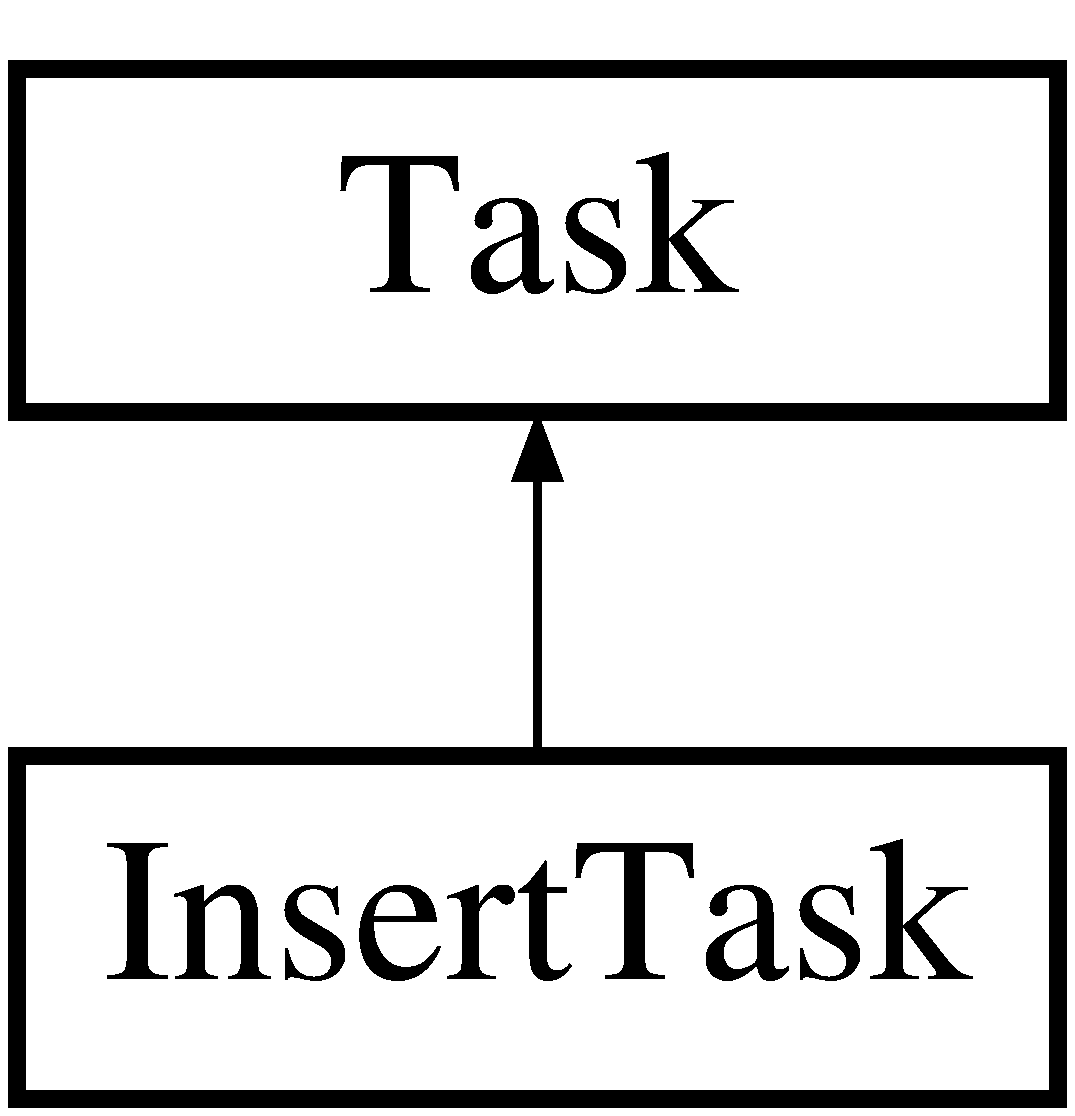
\includegraphics[height=2.000000cm]{class_insert_task}
\end{center}
\end{figure}
\subsection*{Public Member Functions}
\begin{DoxyCompactItemize}
\item 
\mbox{\Hypertarget{class_insert_task_a3ed29b14dbc9f4b4abf01e8db5a7b78e}\label{class_insert_task_a3ed29b14dbc9f4b4abf01e8db5a7b78e}} 
void {\bfseries execute} () override
\end{DoxyCompactItemize}
\subsection*{Protected Member Functions}
\begin{DoxyCompactItemize}
\item 
\mbox{\Hypertarget{class_insert_task_aefda19f32cd281fce586cde640c25f34}\label{class_insert_task_aefda19f32cd281fce586cde640c25f34}} 
{\bfseries L\+E\+M\+O\+N\+D\+B\+\_\+\+Q\+U\+E\+R\+Y\+\_\+\+P\+TR} (\hyperlink{class_insert_query}{Insert\+Query})
\end{DoxyCompactItemize}
\subsection*{Additional Inherited Members}


\subsection{Detailed Description}


Definition at line 18 of file insert\+\_\+query.\+h.



The documentation for this class was generated from the following files\+:\begin{DoxyCompactItemize}
\item 
src/query/data/insert\+\_\+query.\+h\item 
src/query/data/insert\+\_\+query.\+cpp\end{DoxyCompactItemize}

\hypertarget{class_table_1_1_iterator_impl}{}\section{Table\+:\+:Iterator\+Impl$<$ Obj\+Type, Datum\+Iterator $>$ Class Template Reference}
\label{class_table_1_1_iterator_impl}\index{Table\+::\+Iterator\+Impl$<$ Obj\+Type, Datum\+Iterator $>$@{Table\+::\+Iterator\+Impl$<$ Obj\+Type, Datum\+Iterator $>$}}
\subsection*{Public Member Functions}
\begin{DoxyCompactItemize}
\item 
\mbox{\Hypertarget{class_table_1_1_iterator_impl_aca95ed7c924e645c9526fec5e20355b7}\label{class_table_1_1_iterator_impl_aca95ed7c924e645c9526fec5e20355b7}} 
{\bfseries Iterator\+Impl} (Datum\+Iterator datum\+It, const \hyperlink{class_table}{Table} $\ast$t)
\item 
\mbox{\Hypertarget{class_table_1_1_iterator_impl_a464d27cb3ea841cb34107b88aa2f4cf0}\label{class_table_1_1_iterator_impl_a464d27cb3ea841cb34107b88aa2f4cf0}} 
{\bfseries Iterator\+Impl} (const \hyperlink{class_table_1_1_iterator_impl}{Iterator\+Impl} \&)=default
\item 
\mbox{\Hypertarget{class_table_1_1_iterator_impl_a18a3692b208fbb308e1be54009303ee3}\label{class_table_1_1_iterator_impl_a18a3692b208fbb308e1be54009303ee3}} 
{\bfseries Iterator\+Impl} (\hyperlink{class_table_1_1_iterator_impl}{Iterator\+Impl} \&\&) noexcept=default
\item 
\mbox{\Hypertarget{class_table_1_1_iterator_impl_ad4614d4c375981c602e7ee857156ef07}\label{class_table_1_1_iterator_impl_ad4614d4c375981c602e7ee857156ef07}} 
\hyperlink{class_table_1_1_iterator_impl}{Iterator\+Impl} \& {\bfseries operator=} (const \hyperlink{class_table_1_1_iterator_impl}{Iterator\+Impl} \&)=default
\item 
\mbox{\Hypertarget{class_table_1_1_iterator_impl_ac33032203b7058566e732a5d3648254f}\label{class_table_1_1_iterator_impl_ac33032203b7058566e732a5d3648254f}} 
\hyperlink{class_table_1_1_iterator_impl}{Iterator\+Impl} \& {\bfseries operator=} (\hyperlink{class_table_1_1_iterator_impl}{Iterator\+Impl} \&\&) noexcept=default
\item 
\mbox{\Hypertarget{class_table_1_1_iterator_impl_a501bb4348969547c67c2e6a13a042ac8}\label{class_table_1_1_iterator_impl_a501bb4348969547c67c2e6a13a042ac8}} 
pointer {\bfseries operator-\/$>$} ()
\item 
\mbox{\Hypertarget{class_table_1_1_iterator_impl_a50e1787a7699f8920327c5856c28661b}\label{class_table_1_1_iterator_impl_a50e1787a7699f8920327c5856c28661b}} 
reference {\bfseries operator$\ast$} ()
\item 
\mbox{\Hypertarget{class_table_1_1_iterator_impl_a335dcba3f213c98d293879cfa40b6455}\label{class_table_1_1_iterator_impl_a335dcba3f213c98d293879cfa40b6455}} 
\hyperlink{class_table_1_1_iterator_impl}{Iterator\+Impl} \& {\bfseries operator++} ()
\item 
\mbox{\Hypertarget{class_table_1_1_iterator_impl_adbc46557770be1e167c928721618ad31}\label{class_table_1_1_iterator_impl_adbc46557770be1e167c928721618ad31}} 
\hyperlink{class_table_1_1_iterator_impl}{Iterator\+Impl} \& {\bfseries operator-\/-\/} ()
\item 
\mbox{\Hypertarget{class_table_1_1_iterator_impl_a3c641871ff753ffc570960895fcc3bcd}\label{class_table_1_1_iterator_impl_a3c641871ff753ffc570960895fcc3bcd}} 
\hyperlink{class_table_1_1_iterator_impl}{Iterator\+Impl} {\bfseries operator++} (int)
\item 
\mbox{\Hypertarget{class_table_1_1_iterator_impl_af31ce76692f52a13c089e634115c0764}\label{class_table_1_1_iterator_impl_af31ce76692f52a13c089e634115c0764}} 
\hyperlink{class_table_1_1_iterator_impl}{Iterator\+Impl} {\bfseries operator-\/-\/} (int)
\item 
\mbox{\Hypertarget{class_table_1_1_iterator_impl_a893d1f401f2b5b7be1fee2d5639f717e}\label{class_table_1_1_iterator_impl_a893d1f401f2b5b7be1fee2d5639f717e}} 
bool {\bfseries operator==} (const \hyperlink{class_table_1_1_iterator_impl}{Iterator\+Impl} \&other)
\item 
\mbox{\Hypertarget{class_table_1_1_iterator_impl_a88d2bd09c5fde22452f33d56d1384aac}\label{class_table_1_1_iterator_impl_a88d2bd09c5fde22452f33d56d1384aac}} 
bool {\bfseries operator!=} (const \hyperlink{class_table_1_1_iterator_impl}{Iterator\+Impl} \&other)
\item 
\mbox{\Hypertarget{class_table_1_1_iterator_impl_acf14c15ad0007c2bbbee843b2d4e042c}\label{class_table_1_1_iterator_impl_acf14c15ad0007c2bbbee843b2d4e042c}} 
bool {\bfseries operator$<$=} (const \hyperlink{class_table_1_1_iterator_impl}{Iterator\+Impl} \&other)
\item 
\mbox{\Hypertarget{class_table_1_1_iterator_impl_a9bddbd704208fa6fdaefc184fde5c68c}\label{class_table_1_1_iterator_impl_a9bddbd704208fa6fdaefc184fde5c68c}} 
bool {\bfseries operator$>$=} (const \hyperlink{class_table_1_1_iterator_impl}{Iterator\+Impl} \&other)
\item 
\mbox{\Hypertarget{class_table_1_1_iterator_impl_ab35c489b12d3943103d0c7713144fa57}\label{class_table_1_1_iterator_impl_ab35c489b12d3943103d0c7713144fa57}} 
bool {\bfseries operator$<$} (const \hyperlink{class_table_1_1_iterator_impl}{Iterator\+Impl} \&other)
\item 
\mbox{\Hypertarget{class_table_1_1_iterator_impl_a8e36e4e20a6a0da31139a1b57bdfd53a}\label{class_table_1_1_iterator_impl_a8e36e4e20a6a0da31139a1b57bdfd53a}} 
bool {\bfseries operator$>$} (const \hyperlink{class_table_1_1_iterator_impl}{Iterator\+Impl} \&other)
\item 
\mbox{\Hypertarget{class_table_1_1_iterator_impl_a659d539fa5cfbb7e921bd7df846f4bc2}\label{class_table_1_1_iterator_impl_a659d539fa5cfbb7e921bd7df846f4bc2}} 
\hyperlink{class_table_1_1_iterator_impl}{Iterator\+Impl} {\bfseries operator+} (int n)
\item 
\mbox{\Hypertarget{class_table_1_1_iterator_impl_a9ce10f5972218ca9fa27a0aa186e7ecd}\label{class_table_1_1_iterator_impl_a9ce10f5972218ca9fa27a0aa186e7ecd}} 
\hyperlink{class_table_1_1_iterator_impl}{Iterator\+Impl} {\bfseries operator-\/} (int n)
\item 
\mbox{\Hypertarget{class_table_1_1_iterator_impl_a27a9c10d44791c8967cb81047c750db8}\label{class_table_1_1_iterator_impl_a27a9c10d44791c8967cb81047c750db8}} 
\hyperlink{class_table_1_1_iterator_impl}{Iterator\+Impl} \& {\bfseries operator+=} (int n)
\item 
\mbox{\Hypertarget{class_table_1_1_iterator_impl_a17cd1624dbc72cc8e5842a5db4463709}\label{class_table_1_1_iterator_impl_a17cd1624dbc72cc8e5842a5db4463709}} 
\hyperlink{class_table_1_1_iterator_impl}{Iterator\+Impl} \& {\bfseries operator-\/=} (int n)
\end{DoxyCompactItemize}
\subsection*{Friends}
\begin{DoxyCompactItemize}
\item 
\mbox{\Hypertarget{class_table_1_1_iterator_impl_af888815e80064bc9fa1035c6265da86e}\label{class_table_1_1_iterator_impl_af888815e80064bc9fa1035c6265da86e}} 
class {\bfseries Table}
\end{DoxyCompactItemize}


\subsection{Detailed Description}
\subsubsection*{template$<$typename Obj\+Type, typename Datum\+Iterator$>$\newline
class Table\+::\+Iterator\+Impl$<$ Obj\+Type, Datum\+Iterator $>$}



Definition at line 183 of file db\+\_\+table.\+h.



The documentation for this class was generated from the following file\+:\begin{DoxyCompactItemize}
\item 
src/db/db\+\_\+table.\+h\end{DoxyCompactItemize}

\hypertarget{class_list_table_query}{}\section{List\+Table\+Query Class Reference}
\label{class_list_table_query}\index{List\+Table\+Query@{List\+Table\+Query}}
Inheritance diagram for List\+Table\+Query\+:\begin{figure}[H]
\begin{center}
\leavevmode
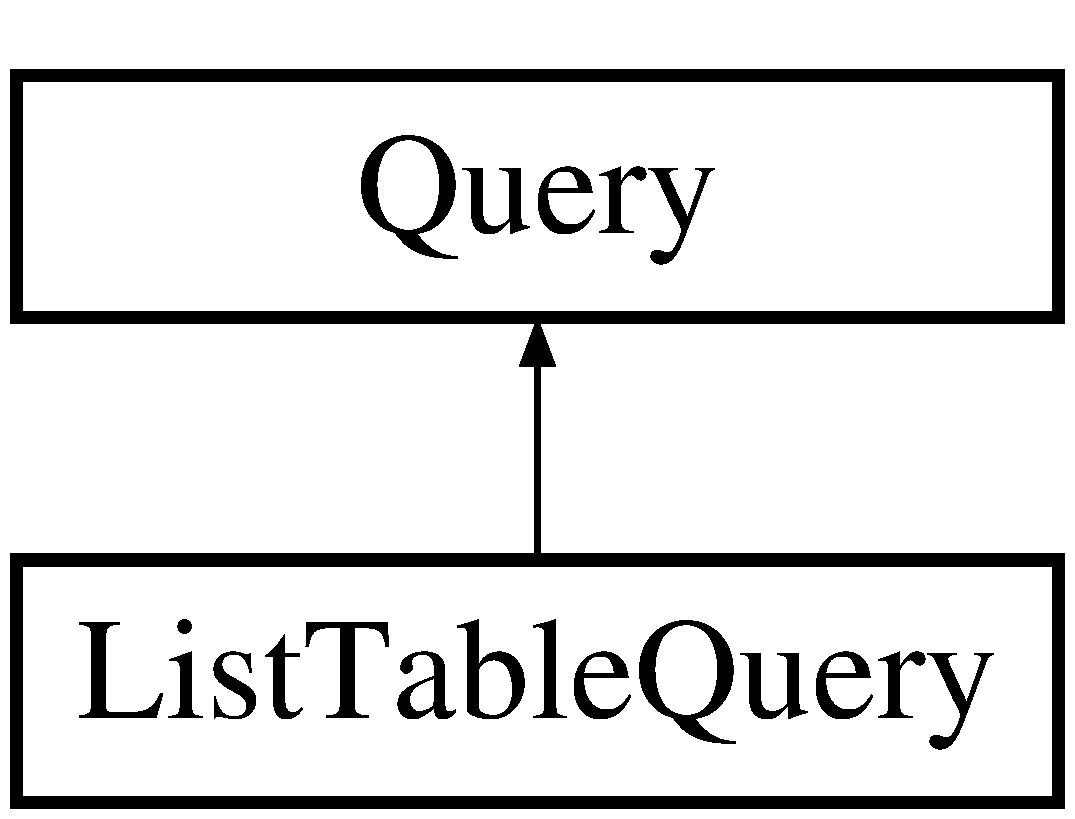
\includegraphics[height=2.000000cm]{class_list_table_query}
\end{center}
\end{figure}
\subsection*{Public Member Functions}
\begin{DoxyCompactItemize}
\item 
\mbox{\Hypertarget{class_list_table_query_a4f663e849be9eea9f3f1c055d478d143}\label{class_list_table_query_a4f663e849be9eea9f3f1c055d478d143}} 
Query\+Result\+::\+Ptr {\bfseries execute} () override
\item 
\mbox{\Hypertarget{class_list_table_query_ac58e1136af9a3304826fb03b7bde819b}\label{class_list_table_query_ac58e1136af9a3304826fb03b7bde819b}} 
std\+::string {\bfseries to\+String} () override
\end{DoxyCompactItemize}
\subsection*{Additional Inherited Members}


\subsection{Detailed Description}


Definition at line 7 of file management\+\_\+query.\+h.



The documentation for this class was generated from the following files\+:\begin{DoxyCompactItemize}
\item 
src/management\+\_\+query.\+h\item 
src/management\+\_\+query.\+cpp\end{DoxyCompactItemize}

\hypertarget{struct_load_from_stream_exception}{}\section{Load\+From\+Stream\+Exception Struct Reference}
\label{struct_load_from_stream_exception}\index{Load\+From\+Stream\+Exception@{Load\+From\+Stream\+Exception}}
Inheritance diagram for Load\+From\+Stream\+Exception\+:\begin{figure}[H]
\begin{center}
\leavevmode
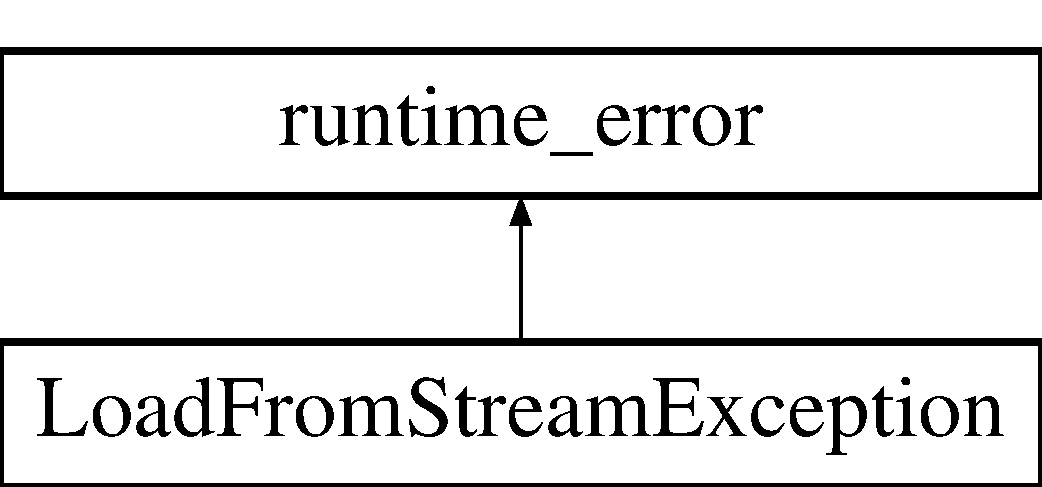
\includegraphics[height=2.000000cm]{struct_load_from_stream_exception}
\end{center}
\end{figure}
\subsection*{Public Member Functions}
\begin{DoxyCompactItemize}
\item 
\mbox{\Hypertarget{struct_load_from_stream_exception_a11fdad41add90b9dab8394a6dadfb106}\label{struct_load_from_stream_exception_a11fdad41add90b9dab8394a6dadfb106}} 
{\bfseries Load\+From\+Stream\+Exception} (const std\+::string \&str)
\end{DoxyCompactItemize}


\subsection{Detailed Description}


Definition at line 41 of file uexception.\+h.



The documentation for this struct was generated from the following file\+:\begin{DoxyCompactItemize}
\item 
src/uexception.\+h\end{DoxyCompactItemize}

\hypertarget{class_load_table_query}{}\section{Load\+Table\+Query Class Reference}
\label{class_load_table_query}\index{Load\+Table\+Query@{Load\+Table\+Query}}
Inheritance diagram for Load\+Table\+Query\+:\begin{figure}[H]
\begin{center}
\leavevmode
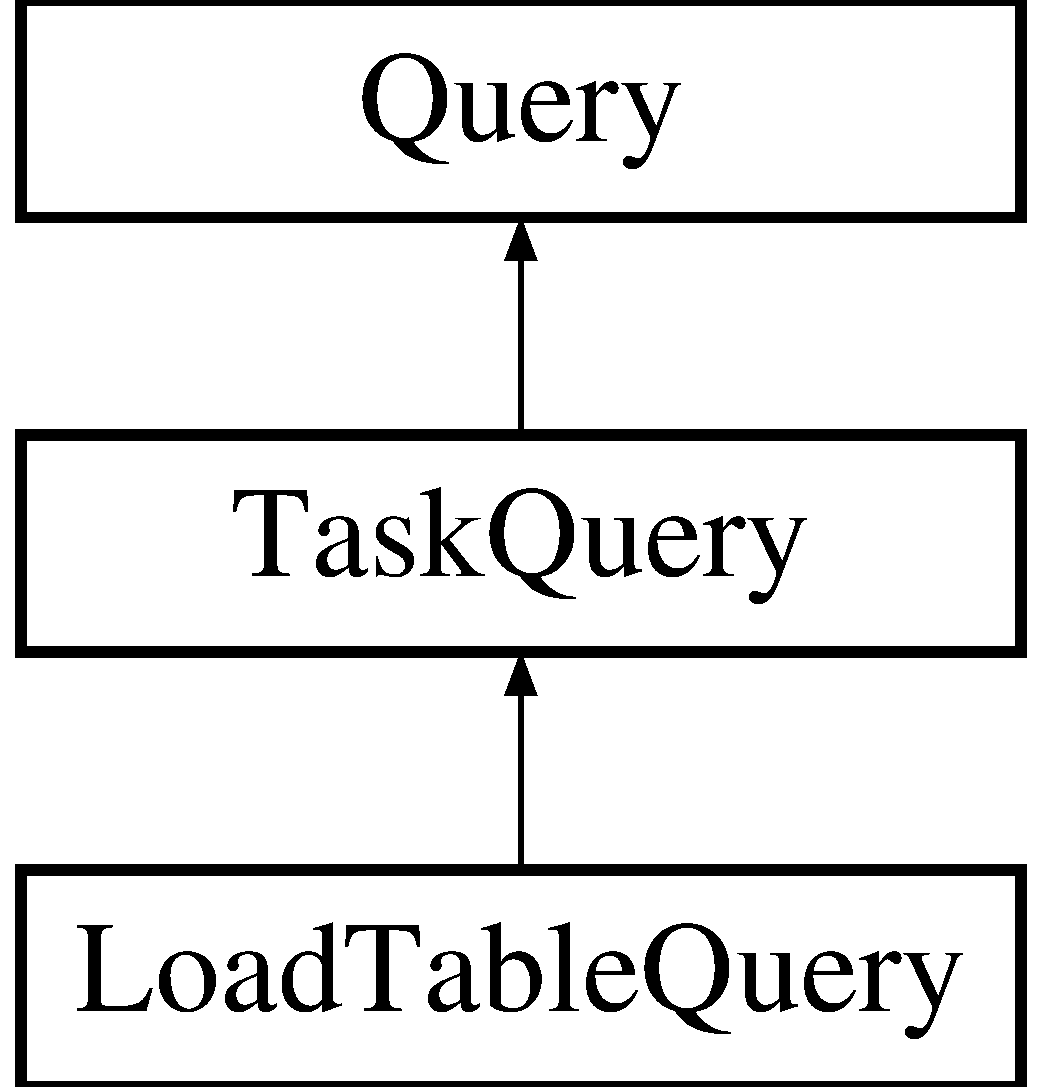
\includegraphics[height=3.000000cm]{class_load_table_query}
\end{center}
\end{figure}
\subsection*{Public Member Functions}
\begin{DoxyCompactItemize}
\item 
\mbox{\Hypertarget{class_load_table_query_ac9169ab007b7027839ee5ac626f1f67b}\label{class_load_table_query_ac9169ab007b7027839ee5ac626f1f67b}} 
{\bfseries L\+E\+M\+O\+N\+D\+B\+\_\+\+Q\+U\+E\+R\+Y\+\_\+\+W\+R\+I\+T\+ER} (true)
\item 
\mbox{\Hypertarget{class_load_table_query_a2dfec4579872e5fe8793d0760ad07547}\label{class_load_table_query_a2dfec4579872e5fe8793d0760ad07547}} 
{\bfseries L\+E\+M\+O\+N\+D\+B\+\_\+\+Q\+U\+E\+R\+Y\+\_\+\+I\+N\+S\+T\+A\+NT} (true)
\item 
\mbox{\Hypertarget{class_load_table_query_a2638e62922f0daff93916b32a6caa4f1}\label{class_load_table_query_a2638e62922f0daff93916b32a6caa4f1}} 
{\bfseries Load\+Table\+Query} (std\+::string table, std\+::string file\+Name)
\item 
\mbox{\Hypertarget{class_load_table_query_a699ce5f313ee96d7f844fd860259812e}\label{class_load_table_query_a699ce5f313ee96d7f844fd860259812e}} 
Query\+Result\+::\+Ptr {\bfseries execute} () override
\item 
\mbox{\Hypertarget{class_load_table_query_a8f8cf237bb4cd6482147b8288c161b50}\label{class_load_table_query_a8f8cf237bb4cd6482147b8288c161b50}} 
std\+::string {\bfseries to\+String} () override
\item 
\mbox{\Hypertarget{class_load_table_query_a64c8e36738ba0d3a85cbe9b8a7c88221}\label{class_load_table_query_a64c8e36738ba0d3a85cbe9b8a7c88221}} 
Query\+Result\+::\+Ptr {\bfseries combine} (int \hyperlink{class_task_query_a3dc3e4c56ddea8ff025239fd9da358d3}{task\+Complete}) override
\end{DoxyCompactItemize}
\subsection*{Friends}
\begin{DoxyCompactItemize}
\item 
\mbox{\Hypertarget{class_load_table_query_aaa7e070e4fcb870c5276bcb77f249378}\label{class_load_table_query_aaa7e070e4fcb870c5276bcb77f249378}} 
class {\bfseries Load\+Table\+Task}
\end{DoxyCompactItemize}
\subsection*{Additional Inherited Members}


\subsection{Detailed Description}


Definition at line 11 of file load\+\_\+table\+\_\+query.\+h.



The documentation for this class was generated from the following files\+:\begin{DoxyCompactItemize}
\item 
src/query/management/load\+\_\+table\+\_\+query.\+h\item 
src/query/management/load\+\_\+table\+\_\+query.\+cpp\end{DoxyCompactItemize}

\hypertarget{class_load_table_task}{}\section{Load\+Table\+Task Class Reference}
\label{class_load_table_task}\index{Load\+Table\+Task@{Load\+Table\+Task}}
Inheritance diagram for Load\+Table\+Task\+:\begin{figure}[H]
\begin{center}
\leavevmode
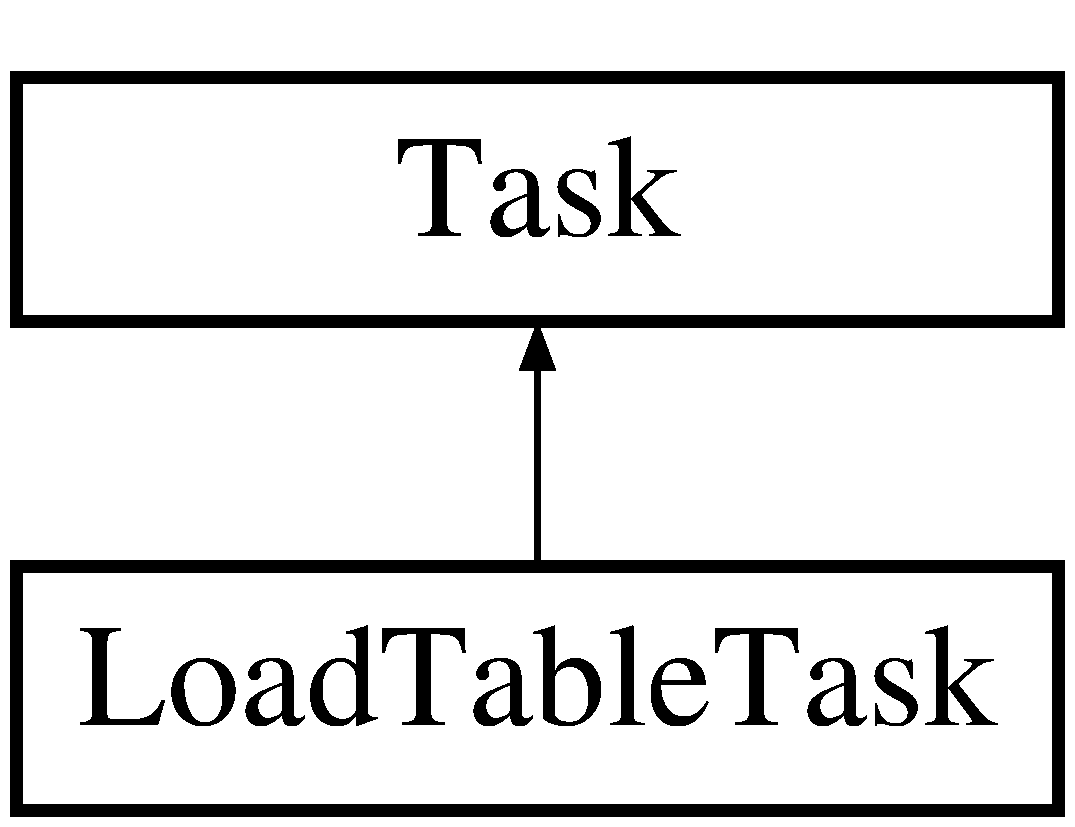
\includegraphics[height=2.000000cm]{class_load_table_task}
\end{center}
\end{figure}
\subsection*{Public Member Functions}
\begin{DoxyCompactItemize}
\item 
\mbox{\Hypertarget{class_load_table_task_ae0516f85ef2c1d2b1f8a2fca17dc1e45}\label{class_load_table_task_ae0516f85ef2c1d2b1f8a2fca17dc1e45}} 
void {\bfseries execute} () override
\end{DoxyCompactItemize}
\subsection*{Protected Member Functions}
\begin{DoxyCompactItemize}
\item 
\mbox{\Hypertarget{class_load_table_task_aa336ffb4e6d23238579a27c993e33263}\label{class_load_table_task_aa336ffb4e6d23238579a27c993e33263}} 
{\bfseries L\+E\+M\+O\+N\+D\+B\+\_\+\+Q\+U\+E\+R\+Y\+\_\+\+P\+TR} (\hyperlink{class_load_table_query}{Load\+Table\+Query})
\end{DoxyCompactItemize}
\subsection*{Additional Inherited Members}


\subsection{Detailed Description}


Definition at line 26 of file load\+\_\+table\+\_\+query.\+h.



The documentation for this class was generated from the following files\+:\begin{DoxyCompactItemize}
\item 
src/query/management/load\+\_\+table\+\_\+query.\+h\item 
src/query/management/load\+\_\+table\+\_\+query.\+cpp\end{DoxyCompactItemize}

\hypertarget{class_max_query}{}\section{Max\+Query Class Reference}
\label{class_max_query}\index{Max\+Query@{Max\+Query}}
Inheritance diagram for Max\+Query\+:\begin{figure}[H]
\begin{center}
\leavevmode
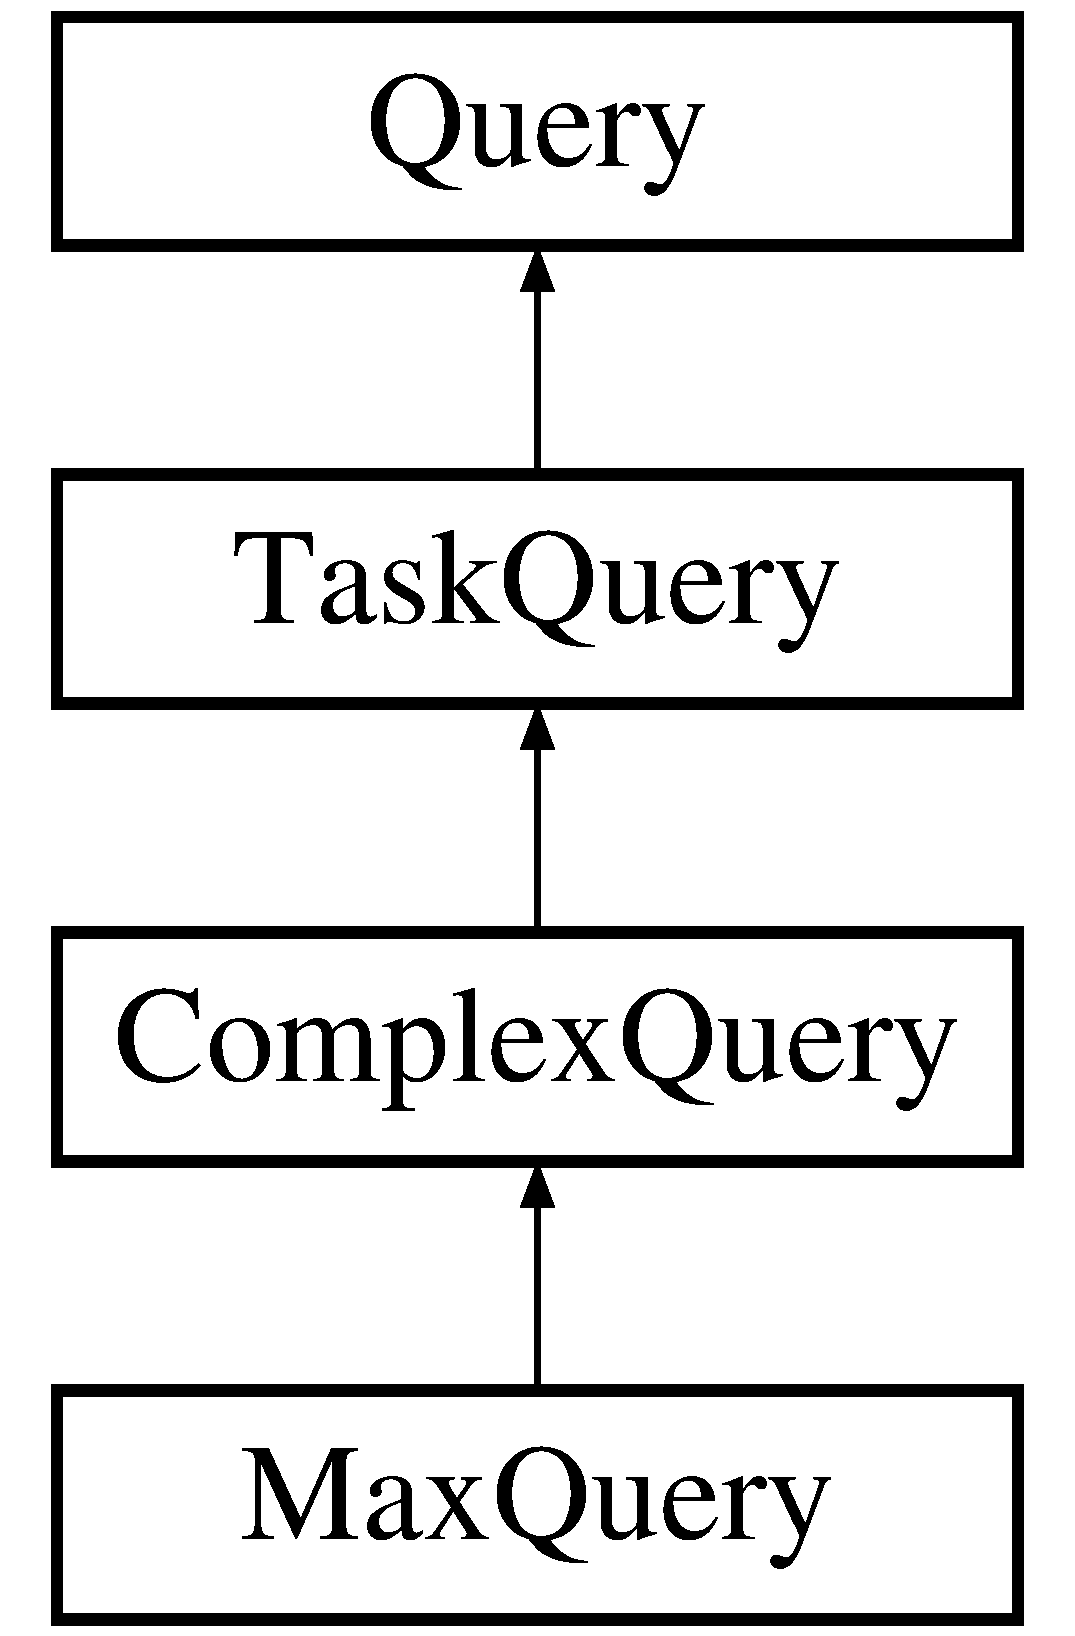
\includegraphics[height=4.000000cm]{class_max_query}
\end{center}
\end{figure}
\subsection*{Public Member Functions}
\begin{DoxyCompactItemize}
\item 
\mbox{\Hypertarget{class_max_query_ac4c1bcca03006eb0dd82cdbbdb6bcbca}\label{class_max_query_ac4c1bcca03006eb0dd82cdbbdb6bcbca}} 
{\bfseries L\+E\+M\+O\+N\+D\+B\+\_\+\+Q\+U\+E\+R\+Y\+\_\+\+W\+R\+I\+T\+ER} (false)
\item 
\mbox{\Hypertarget{class_max_query_a103a8275e8dbdeba69c3982764602e27}\label{class_max_query_a103a8275e8dbdeba69c3982764602e27}} 
Query\+Result\+::\+Ptr {\bfseries execute} () override
\item 
\mbox{\Hypertarget{class_max_query_a03ed2db98d4260ee71341a7bddd88dae}\label{class_max_query_a03ed2db98d4260ee71341a7bddd88dae}} 
std\+::string {\bfseries to\+String} () override
\item 
\mbox{\Hypertarget{class_max_query_a5f6af6472916bf2d1c35bec15a5a70a7}\label{class_max_query_a5f6af6472916bf2d1c35bec15a5a70a7}} 
Query\+Result\+::\+Ptr {\bfseries combine} (int \hyperlink{class_task_query_a3dc3e4c56ddea8ff025239fd9da358d3}{task\+Complete}) override
\end{DoxyCompactItemize}
\subsection*{Protected Member Functions}
\begin{DoxyCompactItemize}
\item 
\mbox{\Hypertarget{class_max_query_a6b7a679b81b0b45571b3f30c850306ba}\label{class_max_query_a6b7a679b81b0b45571b3f30c850306ba}} 
{\bfseries L\+E\+M\+O\+N\+D\+B\+\_\+\+T\+A\+S\+K\+\_\+\+P\+T\+R\+\_\+\+D\+EF} (\hyperlink{class_max_task}{Max\+Task})
\end{DoxyCompactItemize}
\subsection*{Friends}
\begin{DoxyCompactItemize}
\item 
\mbox{\Hypertarget{class_max_query_ac21f840d0c21da4f1f1fa4086450ebaf}\label{class_max_query_ac21f840d0c21da4f1f1fa4086450ebaf}} 
class {\bfseries Max\+Task}
\end{DoxyCompactItemize}
\subsection*{Additional Inherited Members}


\subsection{Detailed Description}


Definition at line 9 of file max\+\_\+query.\+h.



The documentation for this class was generated from the following files\+:\begin{DoxyCompactItemize}
\item 
src/query/data/max\+\_\+query.\+h\item 
src/query/data/max\+\_\+query.\+cpp\end{DoxyCompactItemize}

\hypertarget{class_max_task}{}\section{Max\+Task Class Reference}
\label{class_max_task}\index{Max\+Task@{Max\+Task}}
Inheritance diagram for Max\+Task\+:\begin{figure}[H]
\begin{center}
\leavevmode
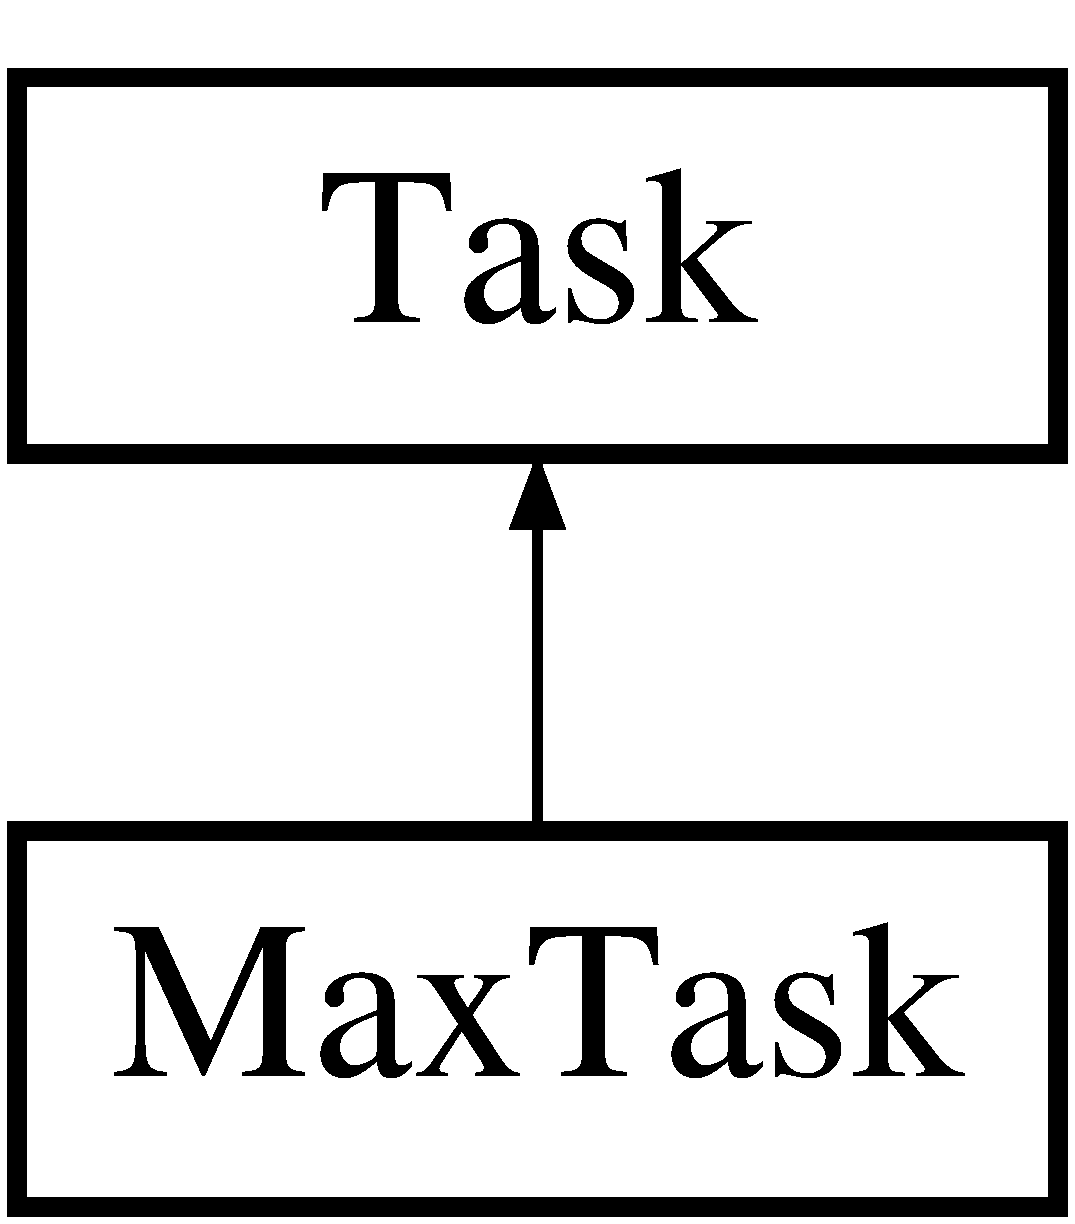
\includegraphics[height=2.000000cm]{class_max_task}
\end{center}
\end{figure}
\subsection*{Public Member Functions}
\begin{DoxyCompactItemize}
\item 
\mbox{\Hypertarget{class_max_task_a874e2dd5c362220b5b64a476425a0ca5}\label{class_max_task_a874e2dd5c362220b5b64a476425a0ca5}} 
void {\bfseries execute} () override
\end{DoxyCompactItemize}
\subsection*{Protected Member Functions}
\begin{DoxyCompactItemize}
\item 
\mbox{\Hypertarget{class_max_task_a3c4011b788369c1a07ff0f2415d166ed}\label{class_max_task_a3c4011b788369c1a07ff0f2415d166ed}} 
{\bfseries L\+E\+M\+O\+N\+D\+B\+\_\+\+Q\+U\+E\+R\+Y\+\_\+\+P\+TR} (\hyperlink{class_max_query}{Max\+Query})
\end{DoxyCompactItemize}
\subsection*{Friends}
\begin{DoxyCompactItemize}
\item 
\mbox{\Hypertarget{class_max_task_a5dd416c177eff007d5ecfaeba2c24505}\label{class_max_task_a5dd416c177eff007d5ecfaeba2c24505}} 
class {\bfseries Max\+Query}
\end{DoxyCompactItemize}
\subsection*{Additional Inherited Members}


\subsection{Detailed Description}


Definition at line 23 of file max\+\_\+query.\+h.



The documentation for this class was generated from the following files\+:\begin{DoxyCompactItemize}
\item 
src/query/data/max\+\_\+query.\+h\item 
src/query/data/max\+\_\+query.\+cpp\end{DoxyCompactItemize}

\hypertarget{class_min_query}{}\section{Min\+Query Class Reference}
\label{class_min_query}\index{Min\+Query@{Min\+Query}}
Inheritance diagram for Min\+Query\+:\begin{figure}[H]
\begin{center}
\leavevmode
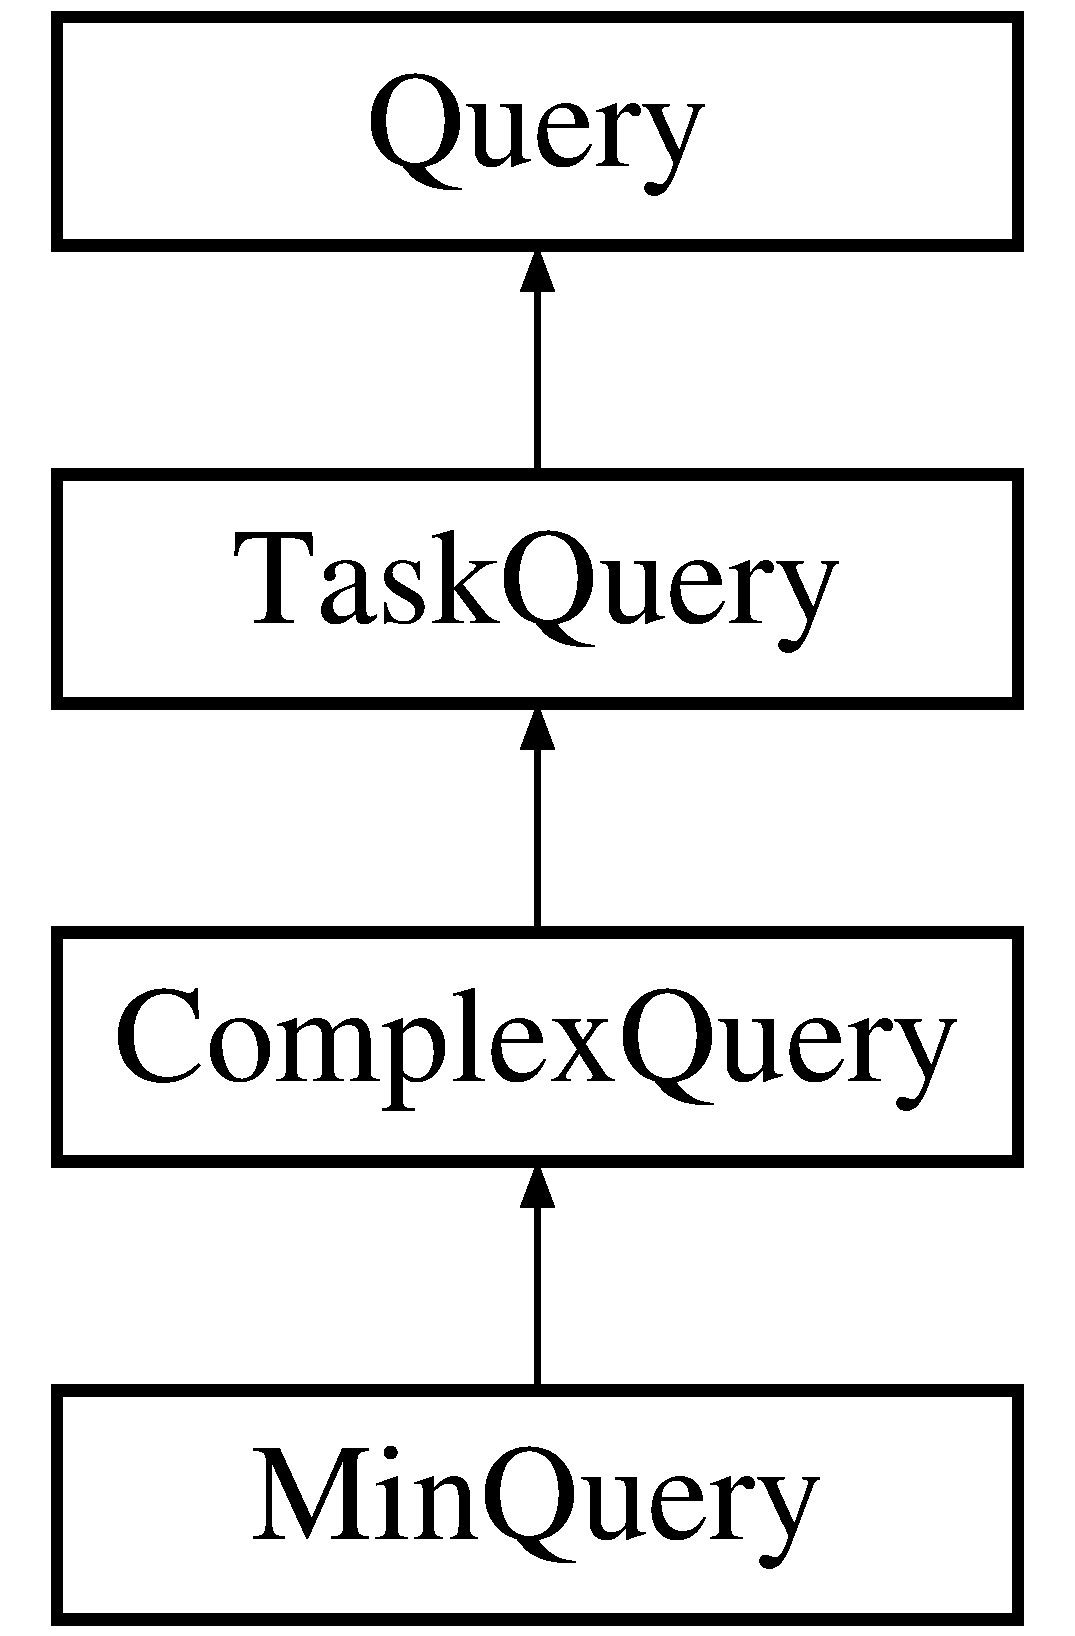
\includegraphics[height=4.000000cm]{class_min_query}
\end{center}
\end{figure}
\subsection*{Public Member Functions}
\begin{DoxyCompactItemize}
\item 
\mbox{\Hypertarget{class_min_query_a42476dc9ba9c545ef508389e2966a573}\label{class_min_query_a42476dc9ba9c545ef508389e2966a573}} 
{\bfseries L\+E\+M\+O\+N\+D\+B\+\_\+\+Q\+U\+E\+R\+Y\+\_\+\+W\+R\+I\+T\+ER} (false)
\item 
\mbox{\Hypertarget{class_min_query_adbb717679491888982d95631438d2820}\label{class_min_query_adbb717679491888982d95631438d2820}} 
Query\+Result\+::\+Ptr {\bfseries execute} () override
\item 
\mbox{\Hypertarget{class_min_query_a46649bffc86277375a11ebfcc9095804}\label{class_min_query_a46649bffc86277375a11ebfcc9095804}} 
std\+::string {\bfseries to\+String} () override
\item 
\mbox{\Hypertarget{class_min_query_acf20a13f11058d63fbf69d9260e4e445}\label{class_min_query_acf20a13f11058d63fbf69d9260e4e445}} 
Query\+Result\+::\+Ptr {\bfseries combine} (int \hyperlink{class_task_query_a3dc3e4c56ddea8ff025239fd9da358d3}{task\+Complete}) override
\end{DoxyCompactItemize}
\subsection*{Protected Member Functions}
\begin{DoxyCompactItemize}
\item 
\mbox{\Hypertarget{class_min_query_a9113a3e2478eeefc09ca74f6df8ee451}\label{class_min_query_a9113a3e2478eeefc09ca74f6df8ee451}} 
{\bfseries L\+E\+M\+O\+N\+D\+B\+\_\+\+T\+A\+S\+K\+\_\+\+P\+T\+R\+\_\+\+D\+EF} (\hyperlink{class_min_task}{Min\+Task})
\end{DoxyCompactItemize}
\subsection*{Friends}
\begin{DoxyCompactItemize}
\item 
\mbox{\Hypertarget{class_min_query_a038d2f25dbf55e5ca51c363822716600}\label{class_min_query_a038d2f25dbf55e5ca51c363822716600}} 
class {\bfseries Min\+Task}
\end{DoxyCompactItemize}
\subsection*{Additional Inherited Members}


\subsection{Detailed Description}


Definition at line 9 of file min\+\_\+query.\+h.



The documentation for this class was generated from the following files\+:\begin{DoxyCompactItemize}
\item 
src/query/data/min\+\_\+query.\+h\item 
src/query/data/min\+\_\+query.\+cpp\end{DoxyCompactItemize}

\hypertarget{class_min_task}{}\section{Min\+Task Class Reference}
\label{class_min_task}\index{Min\+Task@{Min\+Task}}
Inheritance diagram for Min\+Task\+:\begin{figure}[H]
\begin{center}
\leavevmode
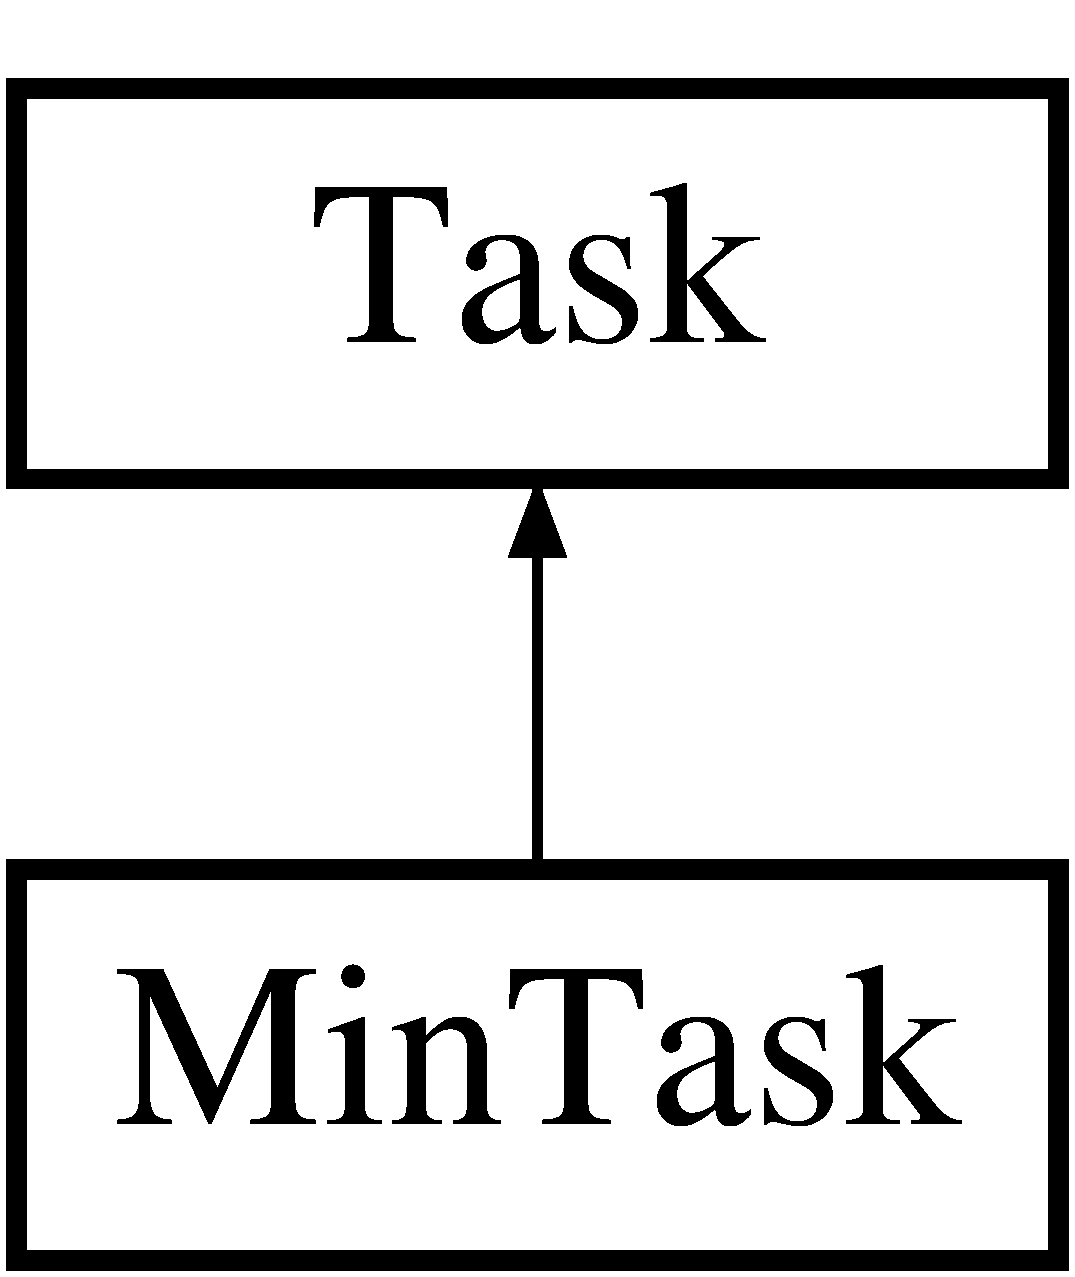
\includegraphics[height=2.000000cm]{class_min_task}
\end{center}
\end{figure}
\subsection*{Public Member Functions}
\begin{DoxyCompactItemize}
\item 
\mbox{\Hypertarget{class_min_task_a63daa4a5eb6eaa16b61ee882613c24cd}\label{class_min_task_a63daa4a5eb6eaa16b61ee882613c24cd}} 
void {\bfseries execute} () override
\end{DoxyCompactItemize}
\subsection*{Protected Member Functions}
\begin{DoxyCompactItemize}
\item 
\mbox{\Hypertarget{class_min_task_a5d7caa2ed72e8af0eef14db1a81a96ef}\label{class_min_task_a5d7caa2ed72e8af0eef14db1a81a96ef}} 
{\bfseries L\+E\+M\+O\+N\+D\+B\+\_\+\+Q\+U\+E\+R\+Y\+\_\+\+P\+TR} (\hyperlink{class_min_query}{Min\+Query})
\end{DoxyCompactItemize}
\subsection*{Friends}
\begin{DoxyCompactItemize}
\item 
\mbox{\Hypertarget{class_min_task_a1cc07b58be7aab7a050da2e024b8ab04}\label{class_min_task_a1cc07b58be7aab7a050da2e024b8ab04}} 
class {\bfseries Min\+Query}
\end{DoxyCompactItemize}
\subsection*{Additional Inherited Members}


\subsection{Detailed Description}


Definition at line 23 of file min\+\_\+query.\+h.



The documentation for this class was generated from the following files\+:\begin{DoxyCompactItemize}
\item 
src/query/data/min\+\_\+query.\+h\item 
src/query/data/min\+\_\+query.\+cpp\end{DoxyCompactItemize}

\hypertarget{struct_multiple_key}{}\section{Multiple\+Key Struct Reference}
\label{struct_multiple_key}\index{Multiple\+Key@{Multiple\+Key}}
Inheritance diagram for Multiple\+Key\+:\begin{figure}[H]
\begin{center}
\leavevmode
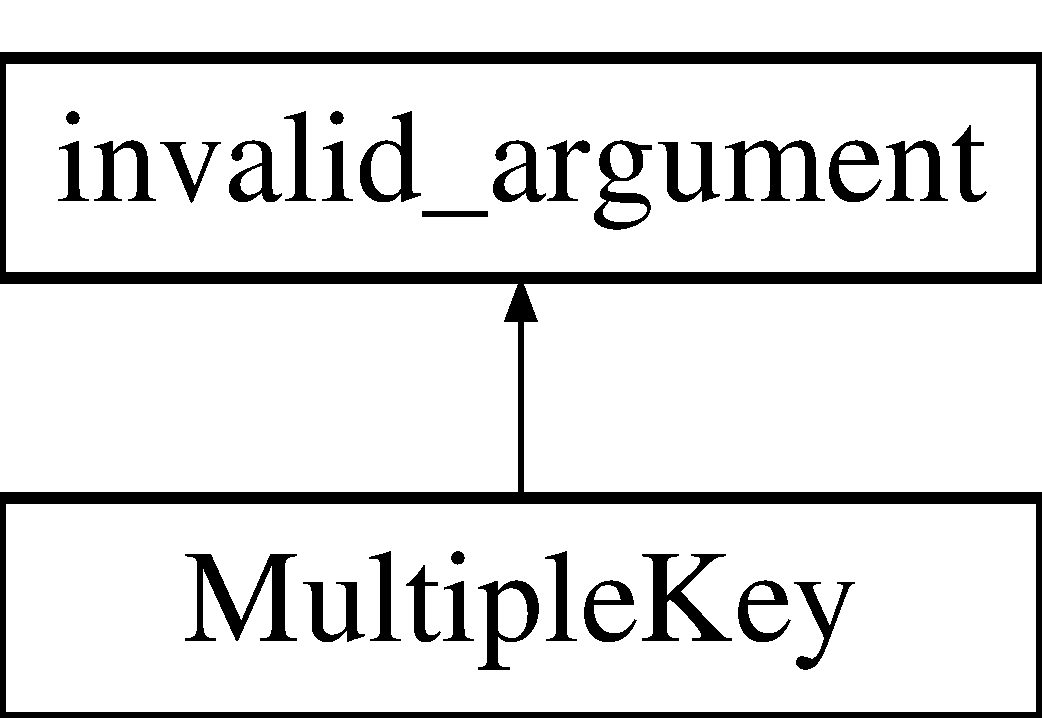
\includegraphics[height=2.000000cm]{struct_multiple_key}
\end{center}
\end{figure}
\subsection*{Public Member Functions}
\begin{DoxyCompactItemize}
\item 
\mbox{\Hypertarget{struct_multiple_key_a383ebd6e3381b47e46cee51b99ae5cc7}\label{struct_multiple_key_a383ebd6e3381b47e46cee51b99ae5cc7}} 
{\bfseries Multiple\+Key} (const std\+::string \&str)
\end{DoxyCompactItemize}


\subsection{Detailed Description}


Definition at line 31 of file uexception.\+h.



The documentation for this struct was generated from the following file\+:\begin{DoxyCompactItemize}
\item 
src/uexception.\+h\end{DoxyCompactItemize}

\hypertarget{class_nop_query}{}\section{Nop\+Query Class Reference}
\label{class_nop_query}\index{Nop\+Query@{Nop\+Query}}
Inheritance diagram for Nop\+Query\+:\begin{figure}[H]
\begin{center}
\leavevmode
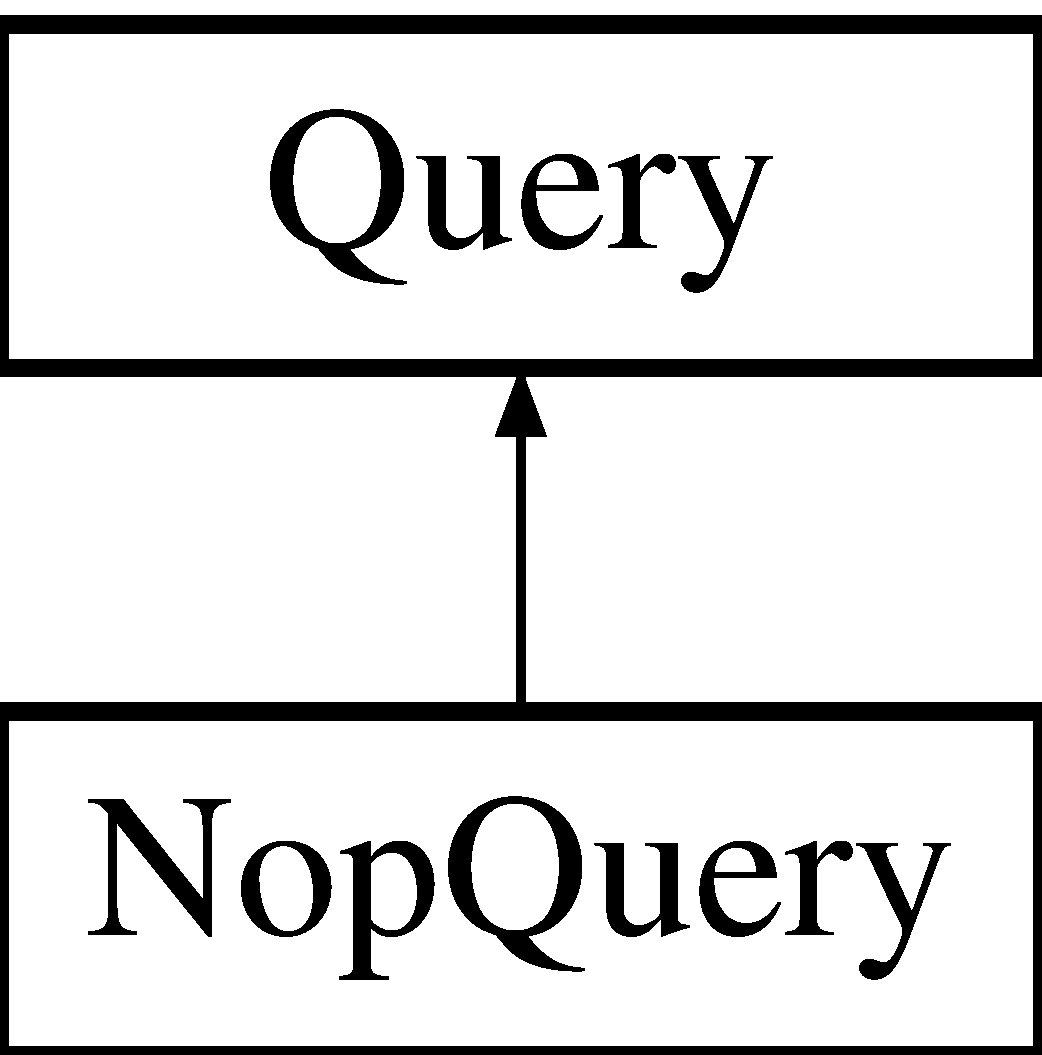
\includegraphics[height=2.000000cm]{class_nop_query}
\end{center}
\end{figure}
\subsection*{Public Member Functions}
\begin{DoxyCompactItemize}
\item 
\mbox{\Hypertarget{class_nop_query_a698ec803e0e04fb153b6b4137ec1da27}\label{class_nop_query_a698ec803e0e04fb153b6b4137ec1da27}} 
Query\+Result\+::\+Ptr {\bfseries execute} () override
\item 
\mbox{\Hypertarget{class_nop_query_abe83dbc25bcc2d4d20fd5699a636e8dc}\label{class_nop_query_abe83dbc25bcc2d4d20fd5699a636e8dc}} 
std\+::string {\bfseries to\+String} () override
\end{DoxyCompactItemize}
\subsection*{Additional Inherited Members}


\subsection{Detailed Description}


Definition at line 22 of file query.\+h.



The documentation for this class was generated from the following file\+:\begin{DoxyCompactItemize}
\item 
src/query/query.\+h\end{DoxyCompactItemize}

\hypertarget{class_null_query_result}{}\section{Null\+Query\+Result Class Reference}
\label{class_null_query_result}\index{Null\+Query\+Result@{Null\+Query\+Result}}
Inheritance diagram for Null\+Query\+Result\+:\begin{figure}[H]
\begin{center}
\leavevmode
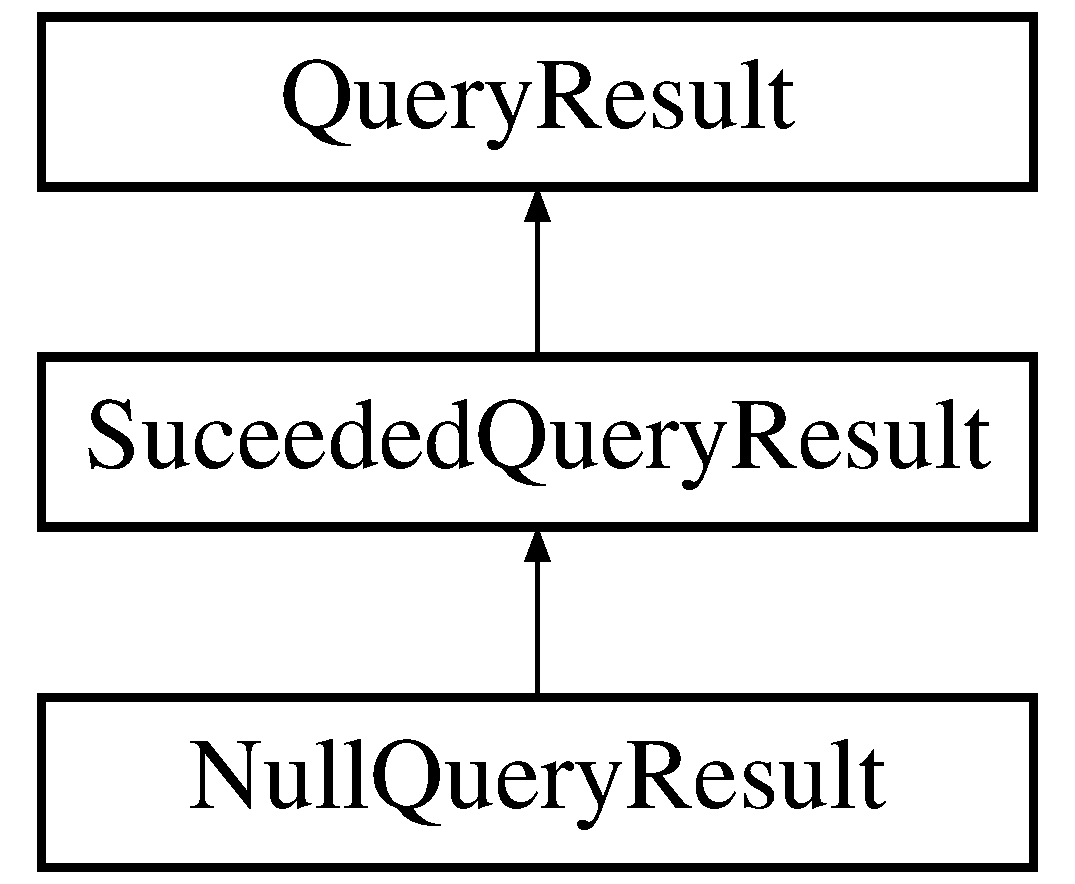
\includegraphics[height=3.000000cm]{class_null_query_result}
\end{center}
\end{figure}
\subsection*{Public Member Functions}
\begin{DoxyCompactItemize}
\item 
\mbox{\Hypertarget{class_null_query_result_ac51149e3f91cc4bc40c05796be2b5815}\label{class_null_query_result_ac51149e3f91cc4bc40c05796be2b5815}} 
std\+::string {\bfseries to\+String} () override
\end{DoxyCompactItemize}
\subsection*{Additional Inherited Members}


\subsection{Detailed Description}


Definition at line 33 of file query\+\_\+results.\+h.



The documentation for this class was generated from the following file\+:\begin{DoxyCompactItemize}
\item 
src/query\+\_\+results.\+h\end{DoxyCompactItemize}

\hypertarget{class_table_1_1_object_impl}{}\section{Table\+:\+:Object\+Impl$<$ Iterator, V\+Type $>$ Class Template Reference}
\label{class_table_1_1_object_impl}\index{Table\+::\+Object\+Impl$<$ Iterator, V\+Type $>$@{Table\+::\+Object\+Impl$<$ Iterator, V\+Type $>$}}


{\ttfamily \#include $<$db\+\_\+table.\+h$>$}

\subsection*{Public Types}
\begin{DoxyCompactItemize}
\item 
\mbox{\Hypertarget{class_table_1_1_object_impl_a892fc764cb681fc422127e79d4ed63fe}\label{class_table_1_1_object_impl_a892fc764cb681fc422127e79d4ed63fe}} 
typedef std\+::unique\+\_\+ptr$<$ \hyperlink{class_table_1_1_object_impl}{Object\+Impl} $>$ {\bfseries Ptr}
\end{DoxyCompactItemize}
\subsection*{Public Member Functions}
\begin{DoxyCompactItemize}
\item 
\mbox{\Hypertarget{class_table_1_1_object_impl_a0ed19396795beaef8460a89b8c35bd22}\label{class_table_1_1_object_impl_a0ed19396795beaef8460a89b8c35bd22}} 
{\bfseries Object\+Impl} (\hyperlink{class_table_1_1_iterator_impl}{Iterator} datum\+It, const \hyperlink{class_table}{Table} $\ast$t)
\item 
\mbox{\Hypertarget{class_table_1_1_object_impl_a0c11ee86de9e1d82a35c09874c652c8e}\label{class_table_1_1_object_impl_a0c11ee86de9e1d82a35c09874c652c8e}} 
{\bfseries Object\+Impl} (const \hyperlink{class_table_1_1_object_impl}{Object\+Impl} \&)=default
\item 
\mbox{\Hypertarget{class_table_1_1_object_impl_a2aeb205c5f5e60849e44b7356a9af11c}\label{class_table_1_1_object_impl_a2aeb205c5f5e60849e44b7356a9af11c}} 
{\bfseries Object\+Impl} (\hyperlink{class_table_1_1_object_impl}{Object\+Impl} \&\&) noexcept=default
\item 
\mbox{\Hypertarget{class_table_1_1_object_impl_ada0904c0c8cab5db6d0e3715e027c779}\label{class_table_1_1_object_impl_ada0904c0c8cab5db6d0e3715e027c779}} 
\hyperlink{class_table_1_1_object_impl}{Object\+Impl} \& {\bfseries operator=} (const \hyperlink{class_table_1_1_object_impl}{Object\+Impl} \&)=default
\item 
\mbox{\Hypertarget{class_table_1_1_object_impl_a2e1856b5d7f2c248587fdafa4f355564}\label{class_table_1_1_object_impl_a2e1856b5d7f2c248587fdafa4f355564}} 
\hyperlink{class_table_1_1_object_impl}{Object\+Impl} \& {\bfseries operator=} (\hyperlink{class_table_1_1_object_impl}{Object\+Impl} \&\&) noexcept=default
\item 
\mbox{\Hypertarget{class_table_1_1_object_impl_ad5686067987189713bb677162b039c3a}\label{class_table_1_1_object_impl_ad5686067987189713bb677162b039c3a}} 
Key\+Type {\bfseries key} () const
\item 
\mbox{\Hypertarget{class_table_1_1_object_impl_a85e6b4a92387a1e45a27655457d8b09f}\label{class_table_1_1_object_impl_a85e6b4a92387a1e45a27655457d8b09f}} 
void {\bfseries set\+Key} (Key\+Type key)
\item 
\mbox{\Hypertarget{class_table_1_1_object_impl_a48dbf990928e6aeda1ba45a8428b2586}\label{class_table_1_1_object_impl_a48dbf990928e6aeda1ba45a8428b2586}} 
V\+Type \& {\bfseries operator\mbox{[}$\,$\mbox{]}} (const Field\+Name\+Type \&\hyperlink{class_table_ab68bc133d1d01f516d0bfb1a9c06e40f}{field}) const
\item 
\mbox{\Hypertarget{class_table_1_1_object_impl_a4b9a905f7ace0a7267997ce3ea5e62af}\label{class_table_1_1_object_impl_a4b9a905f7ace0a7267997ce3ea5e62af}} 
V\+Type \& {\bfseries operator\mbox{[}$\,$\mbox{]}} (const Field\+Index \&index) const
\item 
\mbox{\Hypertarget{class_table_1_1_object_impl_a3e36bfbea13c01dc0a6b9f6ec04587c6}\label{class_table_1_1_object_impl_a3e36bfbea13c01dc0a6b9f6ec04587c6}} 
V\+Type \& {\bfseries get} (const Field\+Name\+Type \&\hyperlink{class_table_ab68bc133d1d01f516d0bfb1a9c06e40f}{field}) const
\item 
\mbox{\Hypertarget{class_table_1_1_object_impl_a86d26919b9bdd0f01a373ab162bf519d}\label{class_table_1_1_object_impl_a86d26919b9bdd0f01a373ab162bf519d}} 
V\+Type \& {\bfseries get} (const Field\+Index \&index) const
\end{DoxyCompactItemize}
\subsection*{Friends}
\begin{DoxyCompactItemize}
\item 
\mbox{\Hypertarget{class_table_1_1_object_impl_af888815e80064bc9fa1035c6265da86e}\label{class_table_1_1_object_impl_af888815e80064bc9fa1035c6265da86e}} 
class {\bfseries Table}
\end{DoxyCompactItemize}


\subsection{Detailed Description}
\subsubsection*{template$<$class Iterator, class V\+Type$>$\newline
class Table\+::\+Object\+Impl$<$ Iterator, V\+Type $>$}

A proxy class that provides abstraction on internal Implementation. Allows independent variation on the Representation for a table object


\begin{DoxyTemplParams}{Template Parameters}
{\em Iterator} & \\
\hline
{\em V\+Type} & \\
\hline
\end{DoxyTemplParams}


Definition at line 122 of file db\+\_\+table.\+h.



The documentation for this class was generated from the following file\+:\begin{DoxyCompactItemize}
\item 
src/db/db\+\_\+table.\+h\end{DoxyCompactItemize}

\hypertarget{class_print_table_query}{}\section{Print\+Table\+Query Class Reference}
\label{class_print_table_query}\index{Print\+Table\+Query@{Print\+Table\+Query}}
Inheritance diagram for Print\+Table\+Query\+:\begin{figure}[H]
\begin{center}
\leavevmode
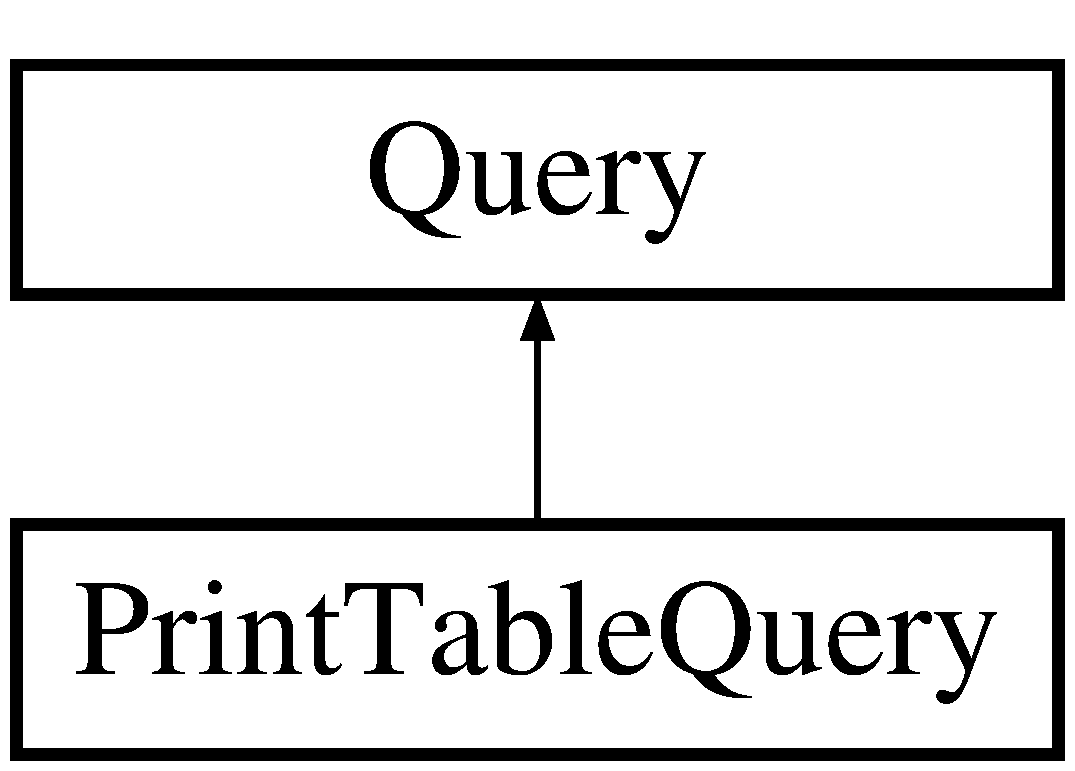
\includegraphics[height=2.000000cm]{class_print_table_query}
\end{center}
\end{figure}
\subsection*{Public Member Functions}
\begin{DoxyCompactItemize}
\item 
\mbox{\Hypertarget{class_print_table_query_a321e11750a9e0e077b3f9411b14dd4a7}\label{class_print_table_query_a321e11750a9e0e077b3f9411b14dd4a7}} 
{\bfseries Print\+Table\+Query} (std\+::string table)
\item 
\mbox{\Hypertarget{class_print_table_query_a0e7005c9ed6b3b870b4f435e74bfa0c7}\label{class_print_table_query_a0e7005c9ed6b3b870b4f435e74bfa0c7}} 
Query\+Result\+::\+Ptr {\bfseries execute} () override
\item 
\mbox{\Hypertarget{class_print_table_query_a143832fd9bbdcb923674a8a2bc9bf83e}\label{class_print_table_query_a143832fd9bbdcb923674a8a2bc9bf83e}} 
std\+::string {\bfseries to\+String} () override
\end{DoxyCompactItemize}
\subsection*{Additional Inherited Members}


\subsection{Detailed Description}


Definition at line 15 of file management\+\_\+query.\+h.



The documentation for this class was generated from the following files\+:\begin{DoxyCompactItemize}
\item 
src/management\+\_\+query.\+h\item 
src/management\+\_\+query.\+cpp\end{DoxyCompactItemize}

\hypertarget{class_query}{}\section{Query Class Reference}
\label{class_query}\index{Query@{Query}}
Inheritance diagram for Query\+:\begin{figure}[H]
\begin{center}
\leavevmode
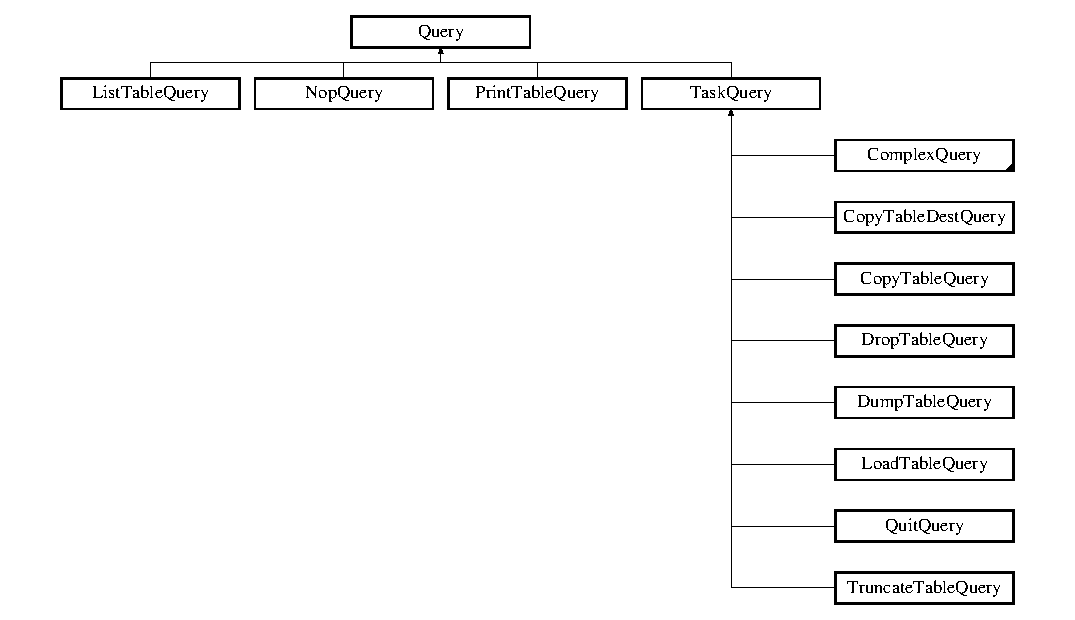
\includegraphics[height=7.887324cm]{class_query}
\end{center}
\end{figure}
\subsection*{Public Types}
\begin{DoxyCompactItemize}
\item 
\mbox{\Hypertarget{class_query_a0a0a7f0fc1097f196ecd56a44baec036}\label{class_query_a0a0a7f0fc1097f196ecd56a44baec036}} 
typedef std\+::unique\+\_\+ptr$<$ \hyperlink{class_query}{Query} $>$ {\bfseries Ptr}
\end{DoxyCompactItemize}
\subsection*{Public Member Functions}
\begin{DoxyCompactItemize}
\item 
\mbox{\Hypertarget{class_query_a758043f481c17af17a48e120ff9ea741}\label{class_query_a758043f481c17af17a48e120ff9ea741}} 
virtual Query\+Result\+::\+Ptr {\bfseries execute} ()=0
\item 
\mbox{\Hypertarget{class_query_afaa6bbe4624620f71e71e259d3f22e31}\label{class_query_afaa6bbe4624620f71e71e259d3f22e31}} 
virtual std\+::string {\bfseries to\+String} ()=0
\item 
\mbox{\Hypertarget{class_query_af9372fbd5d47c9ab56f37a003a9d7953}\label{class_query_af9372fbd5d47c9ab56f37a003a9d7953}} 
virtual Query\+Result\+::\+Ptr {\bfseries combine} (int task\+Complete)
\item 
\mbox{\Hypertarget{class_query_acf7e3add22f3f1317984787fd2e0a251}\label{class_query_acf7e3add22f3f1317984787fd2e0a251}} 
virtual bool {\bfseries is\+Writer} () const =0
\item 
\mbox{\Hypertarget{class_query_aadb2c7d662d4d2a0ee7b5538c4bf90c4}\label{class_query_aadb2c7d662d4d2a0ee7b5538c4bf90c4}} 
virtual bool {\bfseries is\+Instant} () const
\item 
\mbox{\Hypertarget{class_query_a1627ac6e59d31bc9b5b0e1a58315e8b7}\label{class_query_a1627ac6e59d31bc9b5b0e1a58315e8b7}} 
const std\+::string \& {\bfseries get\+Table\+Name} ()
\item 
int \hyperlink{class_query_af59c2164a6ccfe1ad6cc0c6b8ae33938}{get\+Id} () const
\item 
int \hyperlink{class_query_a162c2530d5a3dc048759ec12788b5c90}{init\+Id} (int id)
\end{DoxyCompactItemize}
\subsection*{Protected Attributes}
\begin{DoxyCompactItemize}
\item 
\mbox{\Hypertarget{class_query_ae4aa2f36a804413761d4e131ea407a0b}\label{class_query_ae4aa2f36a804413761d4e131ea407a0b}} 
std\+::string {\bfseries target\+Table}
\item 
\mbox{\Hypertarget{class_query_a3f961ca1a9c82eda79aef080b00a91ef}\label{class_query_a3f961ca1a9c82eda79aef080b00a91ef}} 
int {\bfseries id} = -\/1
\end{DoxyCompactItemize}


\subsection{Detailed Description}


Definition at line 23 of file query\+\_\+base.\+h.



\subsection{Member Function Documentation}
\mbox{\Hypertarget{class_query_af59c2164a6ccfe1ad6cc0c6b8ae33938}\label{class_query_af59c2164a6ccfe1ad6cc0c6b8ae33938}} 
\index{Query@{Query}!get\+Id@{get\+Id}}
\index{get\+Id@{get\+Id}!Query@{Query}}
\subsubsection{\texorpdfstring{get\+Id()}{getId()}}
{\footnotesize\ttfamily int Query\+::get\+Id (\begin{DoxyParamCaption}{ }\end{DoxyParamCaption}) const\hspace{0.3cm}{\ttfamily [inline]}}

get the unique id of this query \begin{DoxyReturn}{Returns}

\end{DoxyReturn}


Definition at line 46 of file query\+\_\+base.\+h.

\mbox{\Hypertarget{class_query_a162c2530d5a3dc048759ec12788b5c90}\label{class_query_a162c2530d5a3dc048759ec12788b5c90}} 
\index{Query@{Query}!init\+Id@{init\+Id}}
\index{init\+Id@{init\+Id}!Query@{Query}}
\subsubsection{\texorpdfstring{init\+Id()}{initId()}}
{\footnotesize\ttfamily int Query\+::init\+Id (\begin{DoxyParamCaption}\item[{int}]{id }\end{DoxyParamCaption})\hspace{0.3cm}{\ttfamily [inline]}}

will only work when first init the query id 
\begin{DoxyParams}{Parameters}
{\em id} & \\
\hline
\end{DoxyParams}
\begin{DoxyReturn}{Returns}

\end{DoxyReturn}


Definition at line 53 of file query\+\_\+base.\+h.



The documentation for this class was generated from the following file\+:\begin{DoxyCompactItemize}
\item 
src/query/query\+\_\+base.\+h\end{DoxyCompactItemize}

\hypertarget{class_query_builder}{}\section{Query\+Builder Class Reference}
\label{class_query_builder}\index{Query\+Builder@{Query\+Builder}}
Inheritance diagram for Query\+Builder\+:\begin{figure}[H]
\begin{center}
\leavevmode
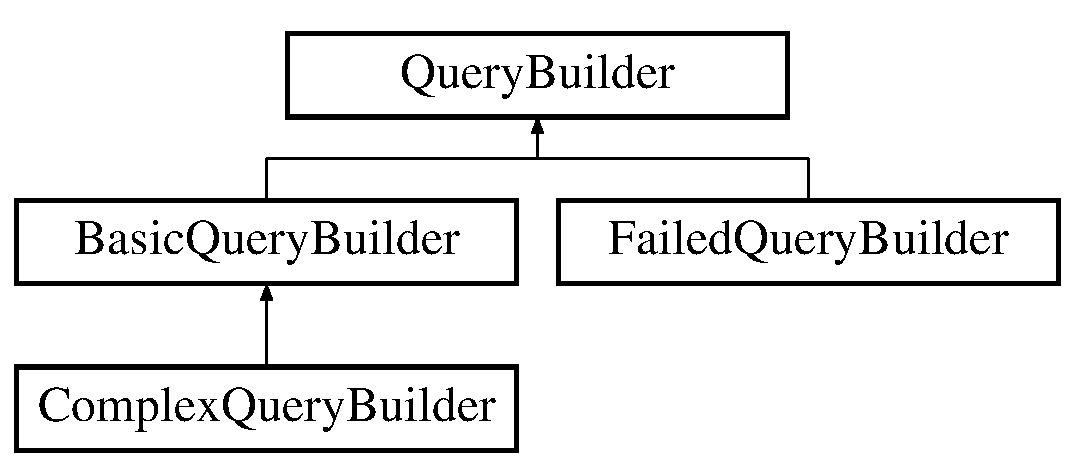
\includegraphics[height=3.000000cm]{class_query_builder}
\end{center}
\end{figure}
\subsection*{Public Types}
\begin{DoxyCompactItemize}
\item 
\mbox{\Hypertarget{class_query_builder_a7398eb0c7e35f50ba1e652f48e56cfe8}\label{class_query_builder_a7398eb0c7e35f50ba1e652f48e56cfe8}} 
typedef std\+::unique\+\_\+ptr$<$ \hyperlink{class_query_builder}{Query\+Builder} $>$ {\bfseries Ptr}
\end{DoxyCompactItemize}
\subsection*{Public Member Functions}
\begin{DoxyCompactItemize}
\item 
\mbox{\Hypertarget{class_query_builder_ac072e9756978c3235e935a46ba7bf3de}\label{class_query_builder_ac072e9756978c3235e935a46ba7bf3de}} 
virtual Query\+::\+Ptr {\bfseries try\+Extract\+Query} (\hyperlink{struct_tokenized_query_string}{Tokenized\+Query\+String} \&query\+String)=0
\item 
\mbox{\Hypertarget{class_query_builder_a45ba6361743c5b9942cf8264662fab62}\label{class_query_builder_a45ba6361743c5b9942cf8264662fab62}} 
virtual void {\bfseries set\+Next} (Ptr \&\&builder)=0
\item 
\mbox{\Hypertarget{class_query_builder_a0be553ef138e355c4f7dd8e5d5711bee}\label{class_query_builder_a0be553ef138e355c4f7dd8e5d5711bee}} 
virtual void {\bfseries clear} ()=0
\end{DoxyCompactItemize}


\subsection{Detailed Description}


Definition at line 15 of file query\+\_\+parser.\+h.



The documentation for this class was generated from the following file\+:\begin{DoxyCompactItemize}
\item 
src/query\+\_\+parser.\+h\end{DoxyCompactItemize}

\hypertarget{class_query_builder_match_failed}{}\section{Query\+Builder\+Match\+Failed Class Reference}
\label{class_query_builder_match_failed}\index{Query\+Builder\+Match\+Failed@{Query\+Builder\+Match\+Failed}}
Inheritance diagram for Query\+Builder\+Match\+Failed\+:\begin{figure}[H]
\begin{center}
\leavevmode
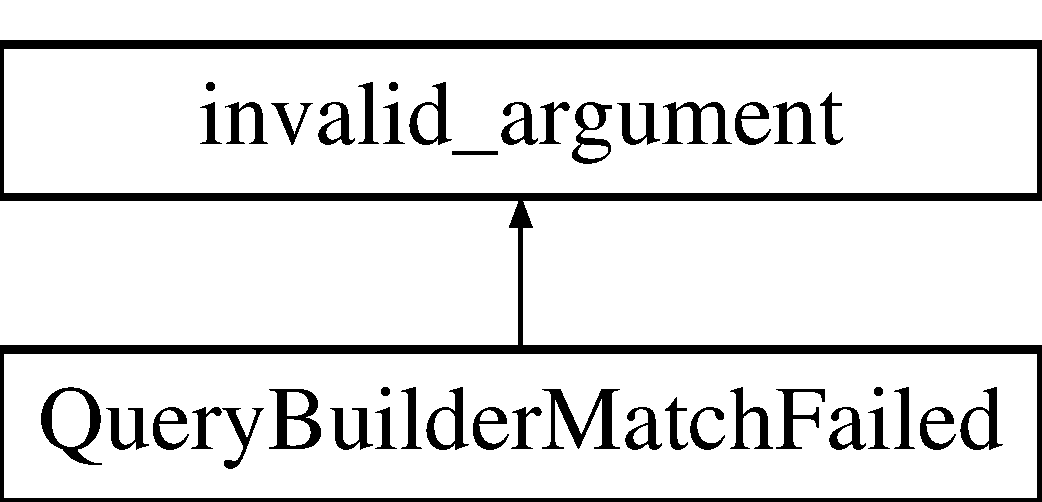
\includegraphics[height=2.000000cm]{class_query_builder_match_failed}
\end{center}
\end{figure}
\subsection*{Public Member Functions}
\begin{DoxyCompactItemize}
\item 
\mbox{\Hypertarget{class_query_builder_match_failed_a821b77ae435862c21634f1e7919210a4}\label{class_query_builder_match_failed_a821b77ae435862c21634f1e7919210a4}} 
{\bfseries Query\+Builder\+Match\+Failed} (const std\+::string \&q\+String)
\end{DoxyCompactItemize}


\subsection{Detailed Description}


Definition at line 56 of file uexception.\+h.



The documentation for this class was generated from the following file\+:\begin{DoxyCompactItemize}
\item 
src/uexception.\+h\end{DoxyCompactItemize}

\hypertarget{struct_query_condition}{}\section{Query\+Condition Struct Reference}
\label{struct_query_condition}\index{Query\+Condition@{Query\+Condition}}
\subsection*{Public Attributes}
\begin{DoxyCompactItemize}
\item 
\mbox{\Hypertarget{struct_query_condition_a9441d3fa04f156825bc33c8e0280f27a}\label{struct_query_condition_a9441d3fa04f156825bc33c8e0280f27a}} 
std\+::string {\bfseries field}
\item 
\mbox{\Hypertarget{struct_query_condition_a12014c8d10ec2042f2af25ed26c57da7}\label{struct_query_condition_a12014c8d10ec2042f2af25ed26c57da7}} 
size\+\_\+t {\bfseries field\+Id}
\item 
\mbox{\Hypertarget{struct_query_condition_ad0d839658ed0d6fcfcf7269d758a0026}\label{struct_query_condition_ad0d839658ed0d6fcfcf7269d758a0026}} 
std\+::string {\bfseries op}
\item 
\mbox{\Hypertarget{struct_query_condition_a7789196c7812945074ed4274cb727522}\label{struct_query_condition_a7789196c7812945074ed4274cb727522}} 
std\+::function$<$ bool(const Table\+::\+Value\+Type \&, const Table\+::\+Value\+Type \&)$>$ {\bfseries comp}
\item 
\mbox{\Hypertarget{struct_query_condition_a9e92d6feb510b6802814b2b188cd334a}\label{struct_query_condition_a9e92d6feb510b6802814b2b188cd334a}} 
std\+::string {\bfseries value}
\item 
\mbox{\Hypertarget{struct_query_condition_aa6171a7b8cb2482381b9de2bb5e8c191}\label{struct_query_condition_aa6171a7b8cb2482381b9de2bb5e8c191}} 
Table\+::\+Value\+Type {\bfseries value\+Parsed}
\end{DoxyCompactItemize}


\subsection{Detailed Description}


Definition at line 13 of file query.\+h.



The documentation for this struct was generated from the following file\+:\begin{DoxyCompactItemize}
\item 
src/query/query.\+h\end{DoxyCompactItemize}

\hypertarget{class_query_parser}{}\section{Query\+Parser Class Reference}
\label{class_query_parser}\index{Query\+Parser@{Query\+Parser}}
\subsection*{Public Member Functions}
\begin{DoxyCompactItemize}
\item 
\mbox{\Hypertarget{class_query_parser_aa0c567455e1a89ce842d869a8bd406fc}\label{class_query_parser_aa0c567455e1a89ce842d869a8bd406fc}} 
Query\+::\+Ptr {\bfseries parse\+Query} (std\+::string query\+String)
\item 
\mbox{\Hypertarget{class_query_parser_aae9e0cedc480e2a2b500b3d8631d0a59}\label{class_query_parser_aae9e0cedc480e2a2b500b3d8631d0a59}} 
void {\bfseries register\+Query\+Builder} (Query\+Builder\+::\+Ptr \&\&q\+Builder)
\end{DoxyCompactItemize}


\subsection{Detailed Description}


Definition at line 27 of file query\+\_\+parser.\+h.



The documentation for this class was generated from the following files\+:\begin{DoxyCompactItemize}
\item 
src/query\+\_\+parser.\+h\item 
src/query\+\_\+parser.\+cpp\end{DoxyCompactItemize}

\hypertarget{class_query_result}{}\section{Query\+Result Class Reference}
\label{class_query_result}\index{Query\+Result@{Query\+Result}}
Inheritance diagram for Query\+Result\+:\begin{figure}[H]
\begin{center}
\leavevmode
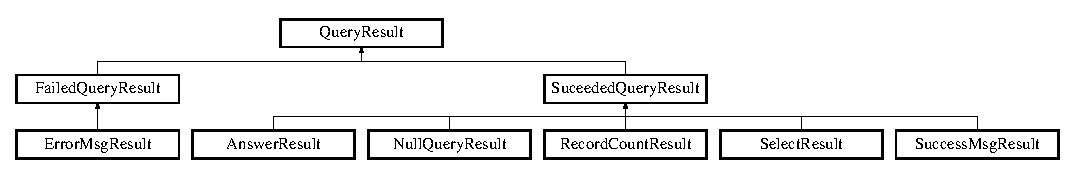
\includegraphics[height=1.904762cm]{class_query_result}
\end{center}
\end{figure}
\subsection*{Public Types}
\begin{DoxyCompactItemize}
\item 
\mbox{\Hypertarget{class_query_result_ad0886002733ecc0922dea3e43d4f7610}\label{class_query_result_ad0886002733ecc0922dea3e43d4f7610}} 
typedef std\+::unique\+\_\+ptr$<$ \hyperlink{class_query_result}{Query\+Result} $>$ {\bfseries Ptr}
\end{DoxyCompactItemize}
\subsection*{Public Member Functions}
\begin{DoxyCompactItemize}
\item 
\mbox{\Hypertarget{class_query_result_a86854387690b31012408c0ed27451db6}\label{class_query_result_a86854387690b31012408c0ed27451db6}} 
virtual bool {\bfseries success} ()=0
\item 
\mbox{\Hypertarget{class_query_result_a98bbf11625700569bd4c1b078f10ceea}\label{class_query_result_a98bbf11625700569bd4c1b078f10ceea}} 
virtual std\+::string {\bfseries to\+String} ()=0
\end{DoxyCompactItemize}


\subsection{Detailed Description}


Definition at line 11 of file query\+\_\+results.\+h.



The documentation for this class was generated from the following file\+:\begin{DoxyCompactItemize}
\item 
src/query\+\_\+results.\+h\end{DoxyCompactItemize}

\hypertarget{class_quit_query}{}\section{Quit\+Query Class Reference}
\label{class_quit_query}\index{Quit\+Query@{Quit\+Query}}
Inheritance diagram for Quit\+Query\+:\begin{figure}[H]
\begin{center}
\leavevmode
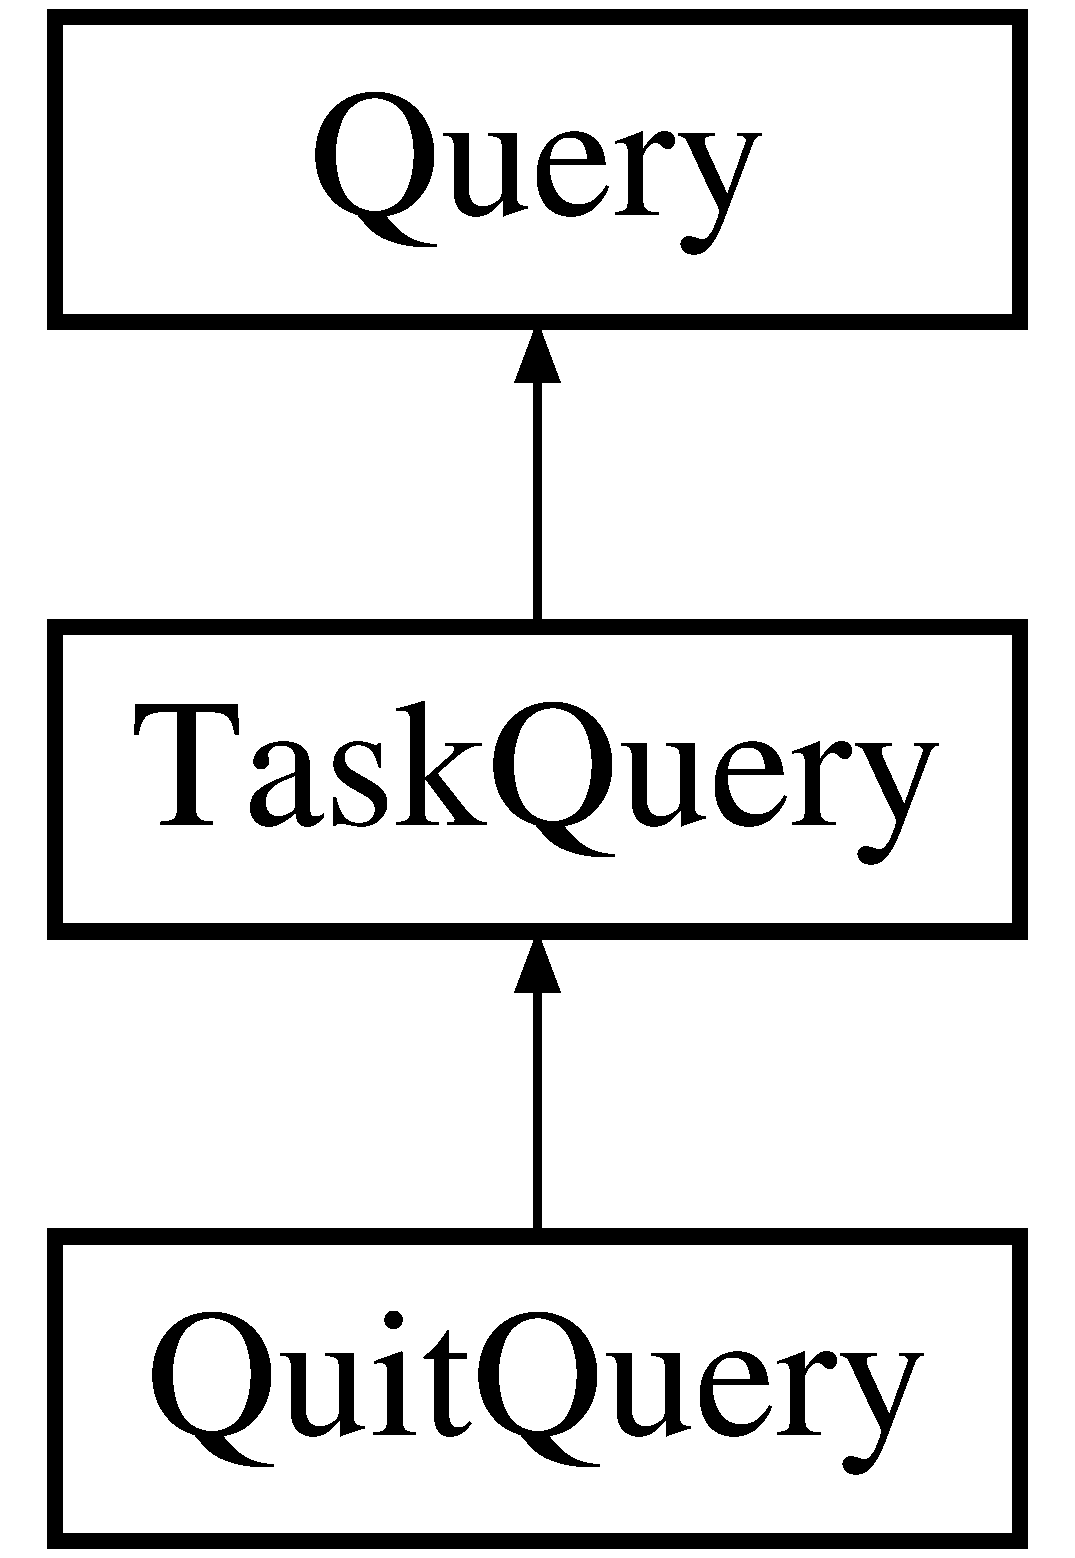
\includegraphics[height=3.000000cm]{class_quit_query}
\end{center}
\end{figure}
\subsection*{Public Member Functions}
\begin{DoxyCompactItemize}
\item 
\mbox{\Hypertarget{class_quit_query_a89c1e8a2fbb5948e627599bb2929de72}\label{class_quit_query_a89c1e8a2fbb5948e627599bb2929de72}} 
Query\+Result\+::\+Ptr {\bfseries execute} () override
\item 
\mbox{\Hypertarget{class_quit_query_a403cc76c4a64c82d19744612e9fb066e}\label{class_quit_query_a403cc76c4a64c82d19744612e9fb066e}} 
std\+::string {\bfseries to\+String} () override
\end{DoxyCompactItemize}
\subsection*{Additional Inherited Members}


\subsection{Detailed Description}


Definition at line 10 of file quit\+\_\+query.\+h.



The documentation for this class was generated from the following files\+:\begin{DoxyCompactItemize}
\item 
src/query/management/quit\+\_\+query.\+h\item 
src/query/management/quit\+\_\+query.\+cpp\end{DoxyCompactItemize}

\hypertarget{class_record_count_result}{}\section{Record\+Count\+Result Class Reference}
\label{class_record_count_result}\index{Record\+Count\+Result@{Record\+Count\+Result}}
Inheritance diagram for Record\+Count\+Result\+:\begin{figure}[H]
\begin{center}
\leavevmode
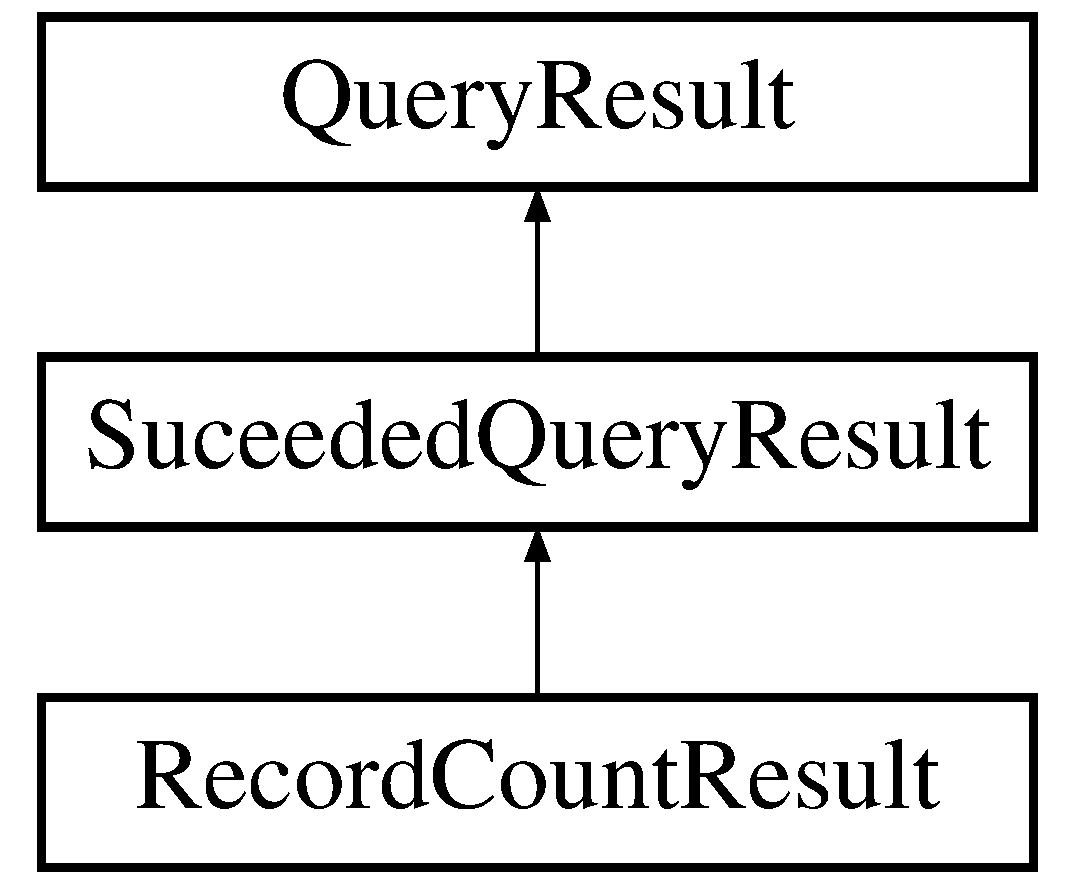
\includegraphics[height=3.000000cm]{class_record_count_result}
\end{center}
\end{figure}
\subsection*{Public Member Functions}
\begin{DoxyCompactItemize}
\item 
\mbox{\Hypertarget{class_record_count_result_aff9926d0e43cd36f44bf306bd80f7f00}\label{class_record_count_result_aff9926d0e43cd36f44bf306bd80f7f00}} 
{\bfseries Record\+Count\+Result} (int count)
\item 
\mbox{\Hypertarget{class_record_count_result_a6d29eca18107e0ef190e458d714c011e}\label{class_record_count_result_a6d29eca18107e0ef190e458d714c011e}} 
std\+::string {\bfseries to\+String} () override
\end{DoxyCompactItemize}
\subsection*{Additional Inherited Members}


\subsection{Detailed Description}


Definition at line 98 of file query\+\_\+results.\+h.



The documentation for this class was generated from the following file\+:\begin{DoxyCompactItemize}
\item 
src/query\+\_\+results.\+h\end{DoxyCompactItemize}

\hypertarget{class_select_query}{}\section{Select\+Query Class Reference}
\label{class_select_query}\index{Select\+Query@{Select\+Query}}
Inheritance diagram for Select\+Query\+:\begin{figure}[H]
\begin{center}
\leavevmode
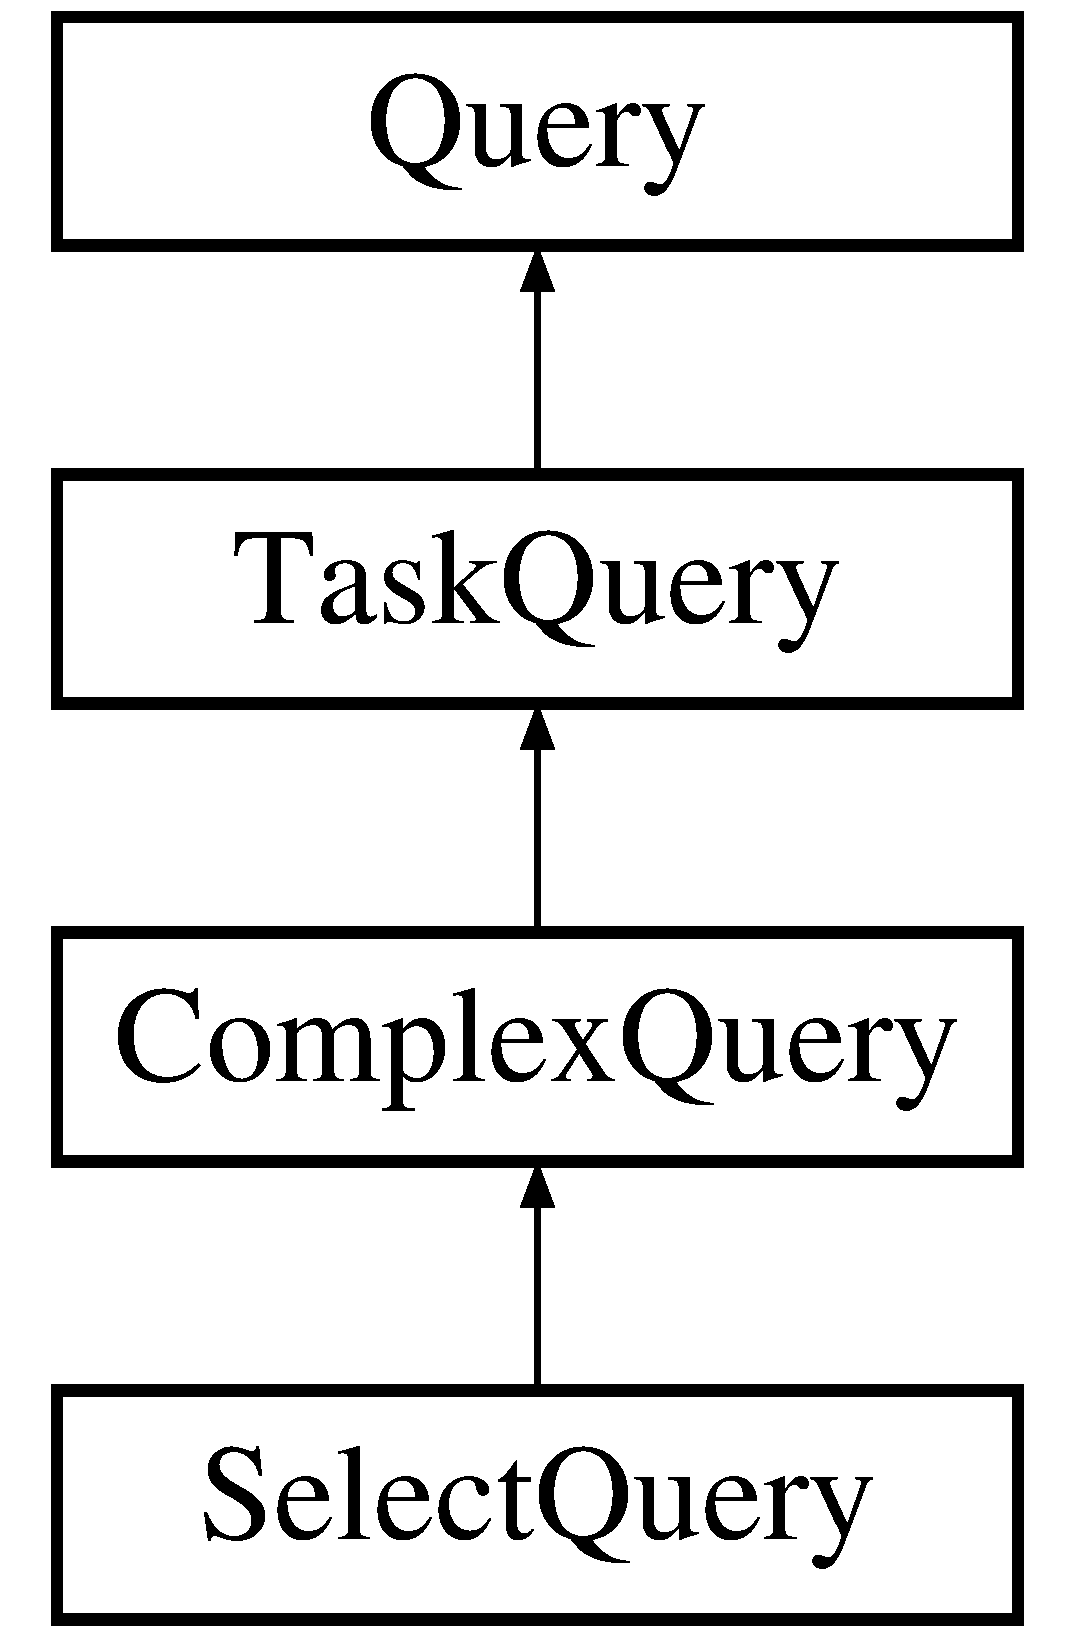
\includegraphics[height=4.000000cm]{class_select_query}
\end{center}
\end{figure}
\subsection*{Public Member Functions}
\begin{DoxyCompactItemize}
\item 
\mbox{\Hypertarget{class_select_query_ab9c596bfd41da9f9af66a514a49503ee}\label{class_select_query_ab9c596bfd41da9f9af66a514a49503ee}} 
{\bfseries L\+E\+M\+O\+N\+D\+B\+\_\+\+Q\+U\+E\+R\+Y\+\_\+\+W\+R\+I\+T\+ER} (false)
\item 
\mbox{\Hypertarget{class_select_query_ac63dcfa4bcde09e85329790f9e774d96}\label{class_select_query_ac63dcfa4bcde09e85329790f9e774d96}} 
Query\+Result\+::\+Ptr {\bfseries execute} () override
\item 
\mbox{\Hypertarget{class_select_query_a7e9bac231930b890df93125575520a7d}\label{class_select_query_a7e9bac231930b890df93125575520a7d}} 
std\+::string {\bfseries to\+String} () override
\item 
\mbox{\Hypertarget{class_select_query_a54b33518896c0f005bfb164025943079}\label{class_select_query_a54b33518896c0f005bfb164025943079}} 
Query\+Result\+::\+Ptr {\bfseries combine} (int \hyperlink{class_task_query_a3dc3e4c56ddea8ff025239fd9da358d3}{task\+Complete}) override
\end{DoxyCompactItemize}
\subsection*{Protected Member Functions}
\begin{DoxyCompactItemize}
\item 
\mbox{\Hypertarget{class_select_query_abcfe881adeb4bef173aa9bee99a0e456}\label{class_select_query_abcfe881adeb4bef173aa9bee99a0e456}} 
{\bfseries L\+E\+M\+O\+N\+D\+B\+\_\+\+T\+A\+S\+K\+\_\+\+P\+T\+R\+\_\+\+D\+EF} (\hyperlink{class_select_task}{Select\+Task})
\end{DoxyCompactItemize}
\subsection*{Friends}
\begin{DoxyCompactItemize}
\item 
\mbox{\Hypertarget{class_select_query_a41f1f8d80f73c7e547ce27261aaa22c0}\label{class_select_query_a41f1f8d80f73c7e547ce27261aaa22c0}} 
class {\bfseries Select\+Task}
\end{DoxyCompactItemize}
\subsection*{Additional Inherited Members}


\subsection{Detailed Description}


Definition at line 13 of file select\+\_\+query.\+h.



The documentation for this class was generated from the following files\+:\begin{DoxyCompactItemize}
\item 
src/query/data/select\+\_\+query.\+h\item 
src/query/data/select\+\_\+query.\+cpp\end{DoxyCompactItemize}

\hypertarget{class_select_result}{}\section{Select\+Result Class Reference}
\label{class_select_result}\index{Select\+Result@{Select\+Result}}
Inheritance diagram for Select\+Result\+:\begin{figure}[H]
\begin{center}
\leavevmode
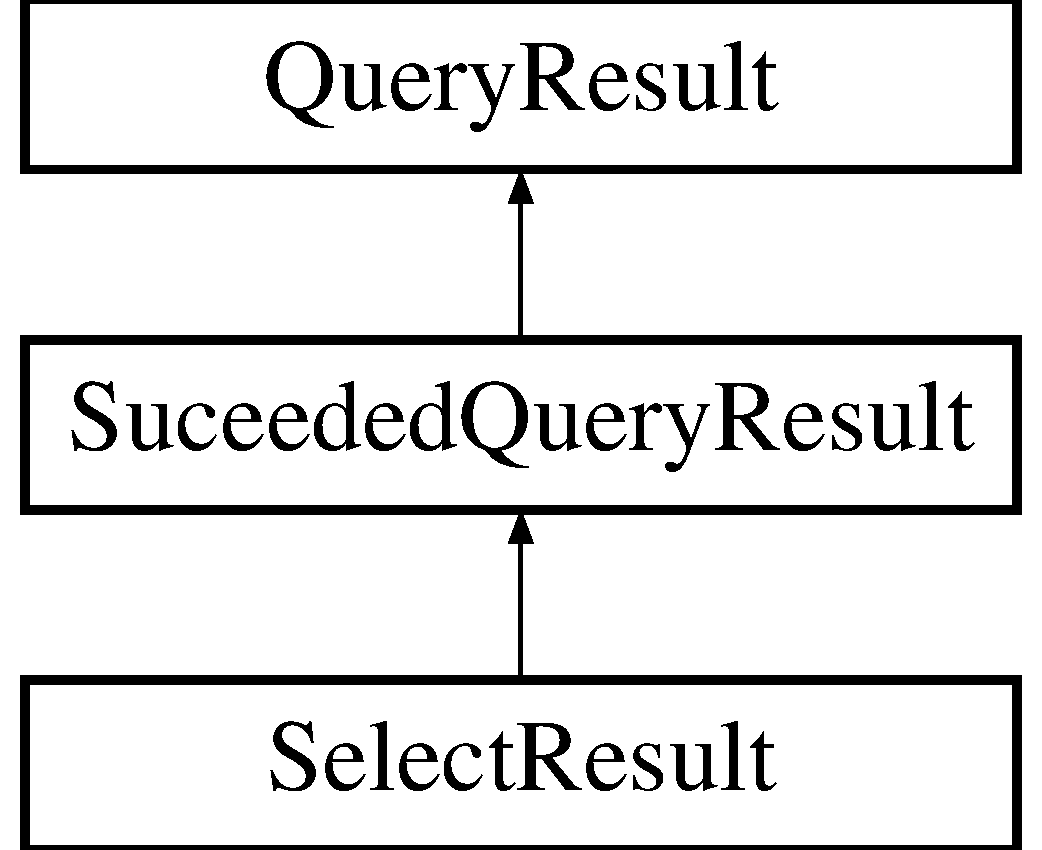
\includegraphics[height=3.000000cm]{class_select_result}
\end{center}
\end{figure}
\subsection*{Public Member Functions}
\begin{DoxyCompactItemize}
\item 
\mbox{\Hypertarget{class_select_result_ac706b6a0c2da988c249eaaff635313d4}\label{class_select_result_ac706b6a0c2da988c249eaaff635313d4}} 
{\bfseries Select\+Result} (std\+::vector$<$ std\+::pair$<$ std\+::string, std\+::vector$<$ int $>$ $>$ $>$ \&\&results)
\item 
\mbox{\Hypertarget{class_select_result_a797ee6d6678401b69ed87d850af06a20}\label{class_select_result_a797ee6d6678401b69ed87d850af06a20}} 
std\+::string {\bfseries to\+String} () override
\end{DoxyCompactItemize}
\subsection*{Additional Inherited Members}


\subsection{Detailed Description}


Definition at line 124 of file query\+\_\+results.\+h.



The documentation for this class was generated from the following file\+:\begin{DoxyCompactItemize}
\item 
src/query\+\_\+results.\+h\end{DoxyCompactItemize}

\hypertarget{class_select_task}{}\section{Select\+Task Class Reference}
\label{class_select_task}\index{Select\+Task@{Select\+Task}}
Inheritance diagram for Select\+Task\+:\begin{figure}[H]
\begin{center}
\leavevmode
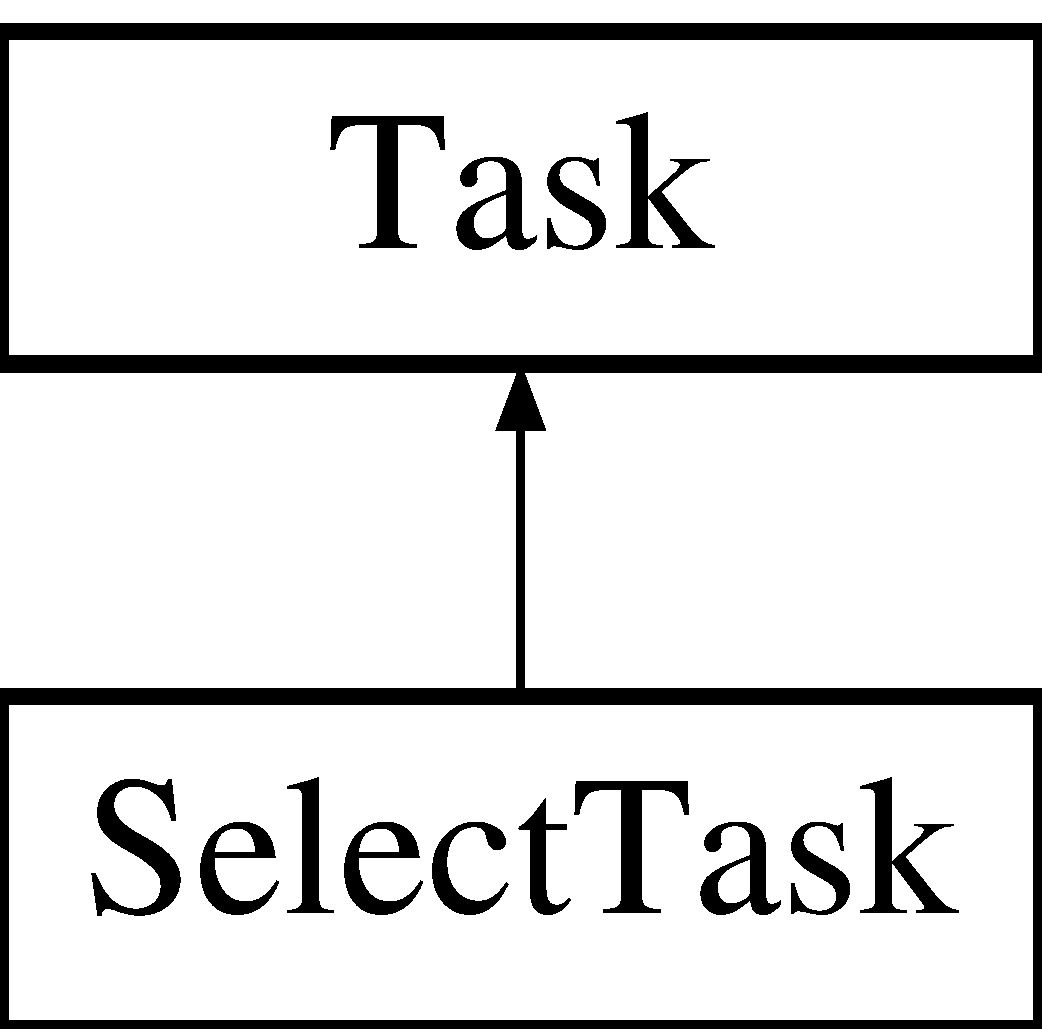
\includegraphics[height=2.000000cm]{class_select_task}
\end{center}
\end{figure}
\subsection*{Public Member Functions}
\begin{DoxyCompactItemize}
\item 
\mbox{\Hypertarget{class_select_task_a4704f6ed1fae988f60424a3f72a8f603}\label{class_select_task_a4704f6ed1fae988f60424a3f72a8f603}} 
void {\bfseries execute} () override
\end{DoxyCompactItemize}
\subsection*{Protected Member Functions}
\begin{DoxyCompactItemize}
\item 
\mbox{\Hypertarget{class_select_task_a9e0d2a32ef67ec0b365cf555924088d6}\label{class_select_task_a9e0d2a32ef67ec0b365cf555924088d6}} 
{\bfseries L\+E\+M\+O\+N\+D\+B\+\_\+\+Q\+U\+E\+R\+Y\+\_\+\+P\+TR} (\hyperlink{class_select_query}{Select\+Query})
\end{DoxyCompactItemize}
\subsection*{Friends}
\begin{DoxyCompactItemize}
\item 
\mbox{\Hypertarget{class_select_task_a4f9a39bcb9cbf2e3e2ca21265d5751fe}\label{class_select_task_a4f9a39bcb9cbf2e3e2ca21265d5751fe}} 
class {\bfseries Select\+Query}
\end{DoxyCompactItemize}
\subsection*{Additional Inherited Members}


\subsection{Detailed Description}


Definition at line 27 of file select\+\_\+query.\+h.



The documentation for this class was generated from the following files\+:\begin{DoxyCompactItemize}
\item 
src/query/data/select\+\_\+query.\+h\item 
src/query/data/select\+\_\+query.\+cpp\end{DoxyCompactItemize}

\hypertarget{class_sub_query}{}\section{Sub\+Query Class Reference}
\label{class_sub_query}\index{Sub\+Query@{Sub\+Query}}
Inheritance diagram for Sub\+Query\+:\begin{figure}[H]
\begin{center}
\leavevmode
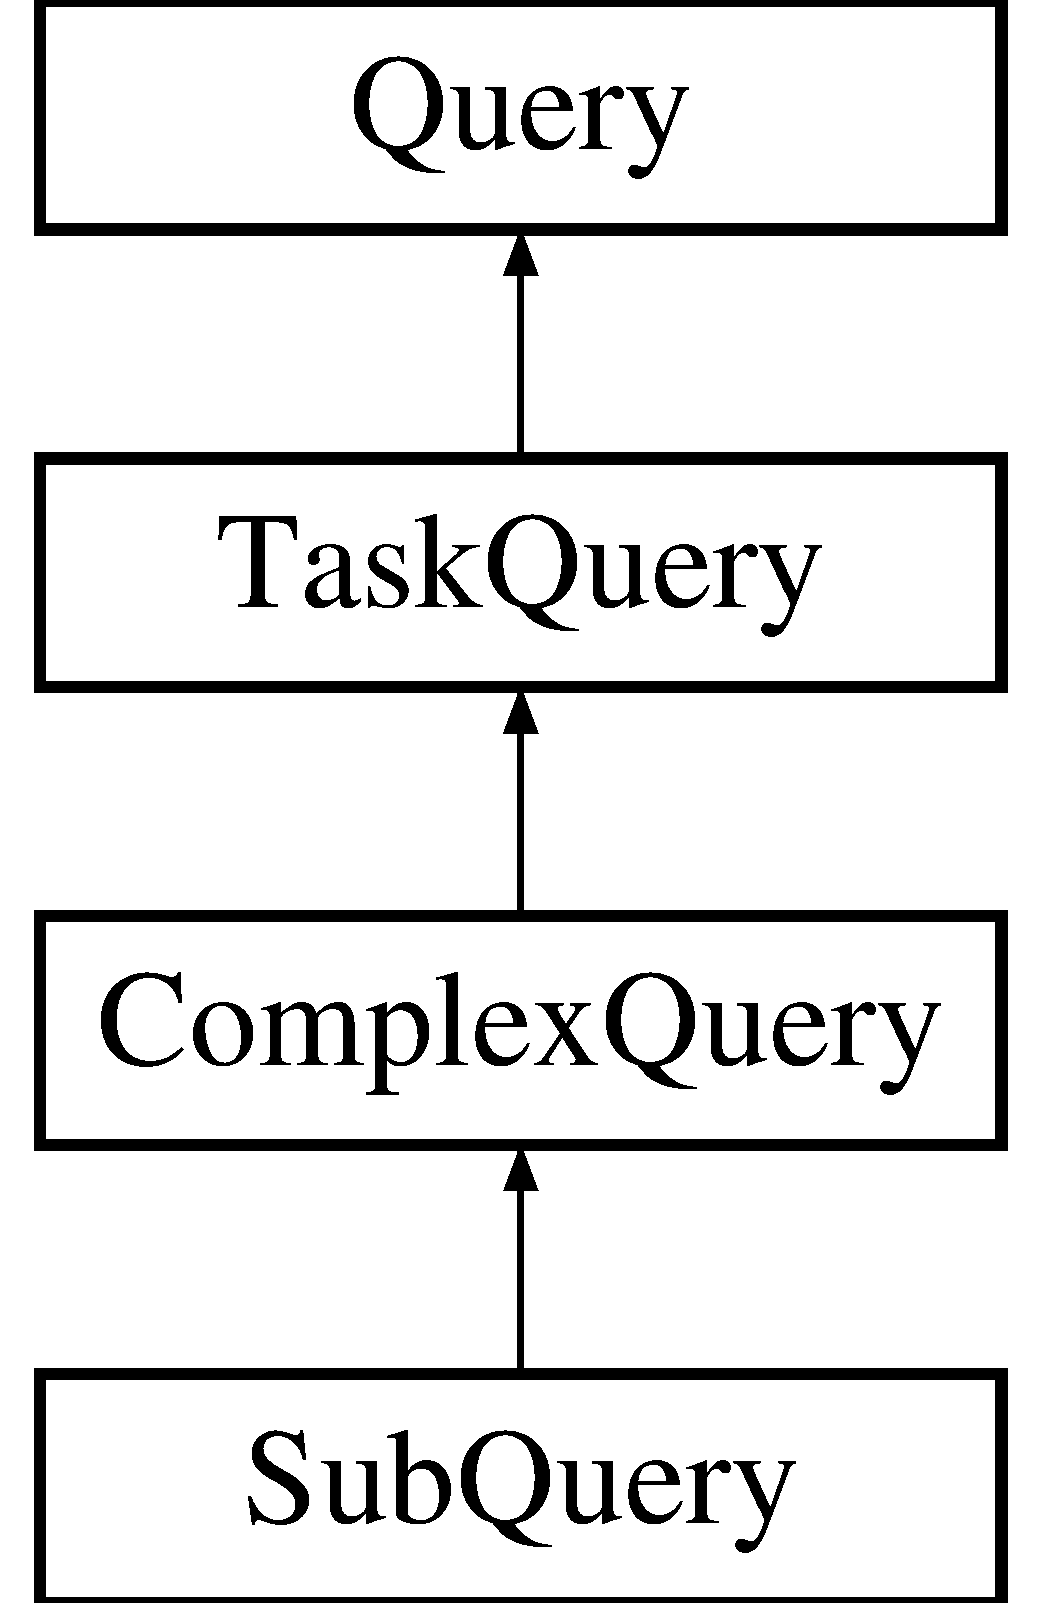
\includegraphics[height=4.000000cm]{class_sub_query}
\end{center}
\end{figure}
\subsection*{Public Member Functions}
\begin{DoxyCompactItemize}
\item 
\mbox{\Hypertarget{class_sub_query_ac4f2c193575f74f0cfba4776bdac56f1}\label{class_sub_query_ac4f2c193575f74f0cfba4776bdac56f1}} 
{\bfseries L\+E\+M\+O\+N\+D\+B\+\_\+\+Q\+U\+E\+R\+Y\+\_\+\+W\+R\+I\+T\+ER} (true)
\item 
\mbox{\Hypertarget{class_sub_query_a84538be0dc7751213fb814ee17fa59d4}\label{class_sub_query_a84538be0dc7751213fb814ee17fa59d4}} 
Query\+Result\+::\+Ptr {\bfseries execute} () override
\item 
\mbox{\Hypertarget{class_sub_query_a3644fa8936b941009682a145e5a573aa}\label{class_sub_query_a3644fa8936b941009682a145e5a573aa}} 
std\+::string {\bfseries to\+String} () override
\item 
\mbox{\Hypertarget{class_sub_query_ab43ddfaec5faaf5914eaa70a3b34d0c1}\label{class_sub_query_ab43ddfaec5faaf5914eaa70a3b34d0c1}} 
Query\+Result\+::\+Ptr {\bfseries combine} (int \hyperlink{class_task_query_a3dc3e4c56ddea8ff025239fd9da358d3}{task\+Complete}) override
\end{DoxyCompactItemize}
\subsection*{Protected Member Functions}
\begin{DoxyCompactItemize}
\item 
\mbox{\Hypertarget{class_sub_query_a3908cdfe9687a134a157a3b1f592419f}\label{class_sub_query_a3908cdfe9687a134a157a3b1f592419f}} 
{\bfseries L\+E\+M\+O\+N\+D\+B\+\_\+\+T\+A\+S\+K\+\_\+\+P\+T\+R\+\_\+\+D\+EF} (\hyperlink{class_sub_task}{Sub\+Task})
\end{DoxyCompactItemize}
\subsection*{Friends}
\begin{DoxyCompactItemize}
\item 
\mbox{\Hypertarget{class_sub_query_a288acc5f848042d157069762b94173a7}\label{class_sub_query_a288acc5f848042d157069762b94173a7}} 
class {\bfseries Sub\+Task}
\end{DoxyCompactItemize}
\subsection*{Additional Inherited Members}


\subsection{Detailed Description}


Definition at line 9 of file sub\+\_\+query.\+h.



The documentation for this class was generated from the following files\+:\begin{DoxyCompactItemize}
\item 
src/query/data/sub\+\_\+query.\+h\item 
src/query/data/sub\+\_\+query.\+cpp\end{DoxyCompactItemize}

\hypertarget{class_sub_task}{}\section{Sub\+Task Class Reference}
\label{class_sub_task}\index{Sub\+Task@{Sub\+Task}}
Inheritance diagram for Sub\+Task\+:\begin{figure}[H]
\begin{center}
\leavevmode
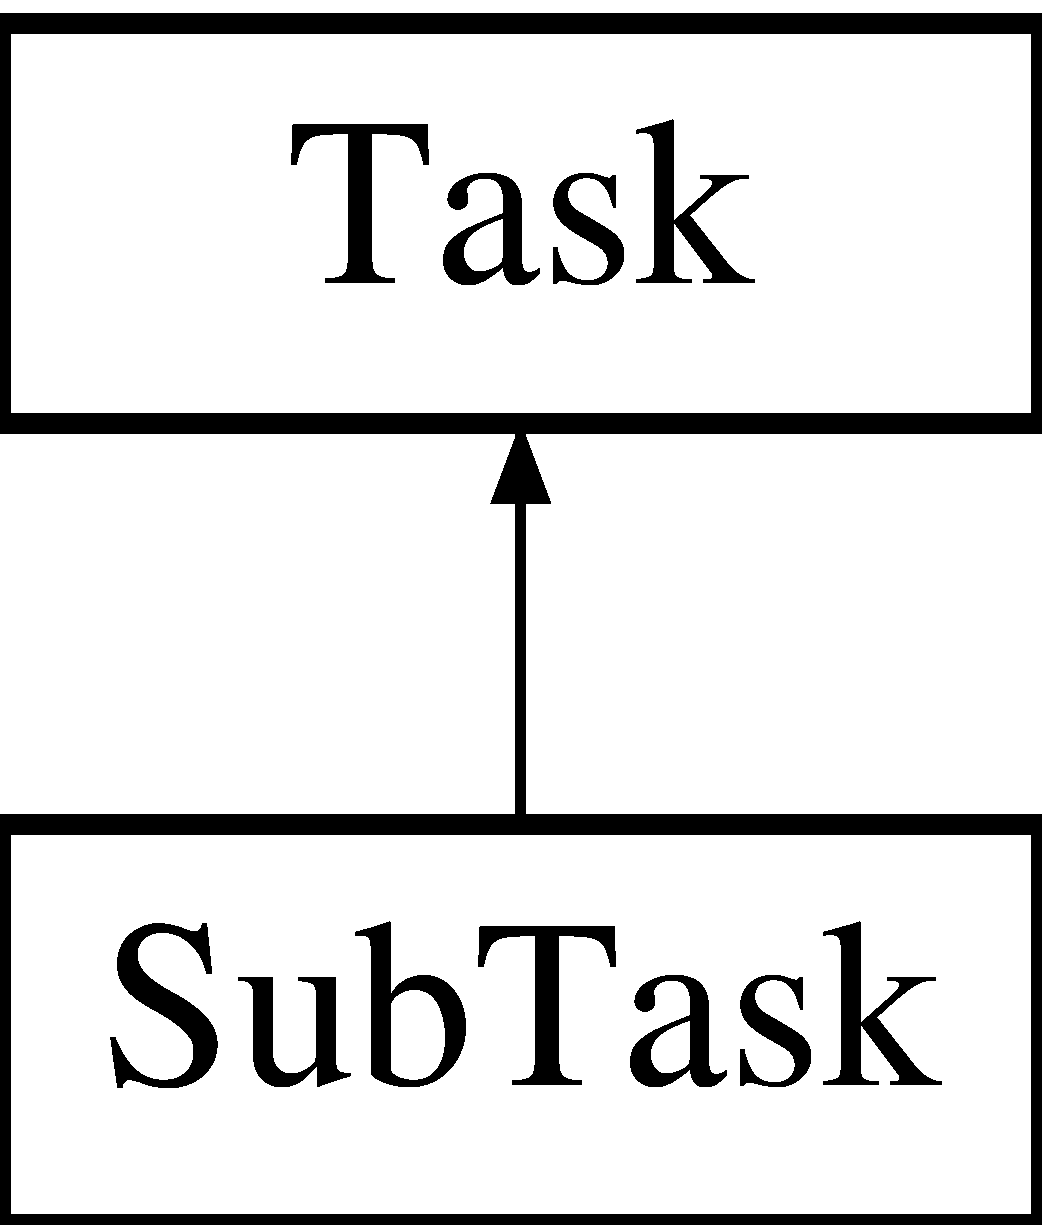
\includegraphics[height=2.000000cm]{class_sub_task}
\end{center}
\end{figure}
\subsection*{Public Member Functions}
\begin{DoxyCompactItemize}
\item 
\mbox{\Hypertarget{class_sub_task_a44a895086552289bb7d9908e4b84d667}\label{class_sub_task_a44a895086552289bb7d9908e4b84d667}} 
void {\bfseries execute} () override
\end{DoxyCompactItemize}
\subsection*{Protected Member Functions}
\begin{DoxyCompactItemize}
\item 
\mbox{\Hypertarget{class_sub_task_aca474662ed1f263e888cf0465e235395}\label{class_sub_task_aca474662ed1f263e888cf0465e235395}} 
{\bfseries L\+E\+M\+O\+N\+D\+B\+\_\+\+Q\+U\+E\+R\+Y\+\_\+\+P\+TR} (\hyperlink{class_sub_query}{Sub\+Query})
\end{DoxyCompactItemize}
\subsection*{Friends}
\begin{DoxyCompactItemize}
\item 
\mbox{\Hypertarget{class_sub_task_adf6a6118fa63fe11409653e2f0a156c9}\label{class_sub_task_adf6a6118fa63fe11409653e2f0a156c9}} 
class {\bfseries Sub\+Query}
\end{DoxyCompactItemize}
\subsection*{Additional Inherited Members}


\subsection{Detailed Description}


Definition at line 23 of file sub\+\_\+query.\+h.



The documentation for this class was generated from the following files\+:\begin{DoxyCompactItemize}
\item 
src/query/data/sub\+\_\+query.\+h\item 
src/query/data/sub\+\_\+query.\+cpp\end{DoxyCompactItemize}

\hypertarget{class_success_msg_result}{}\section{Success\+Msg\+Result Class Reference}
\label{class_success_msg_result}\index{Success\+Msg\+Result@{Success\+Msg\+Result}}
Inheritance diagram for Success\+Msg\+Result\+:\begin{figure}[H]
\begin{center}
\leavevmode
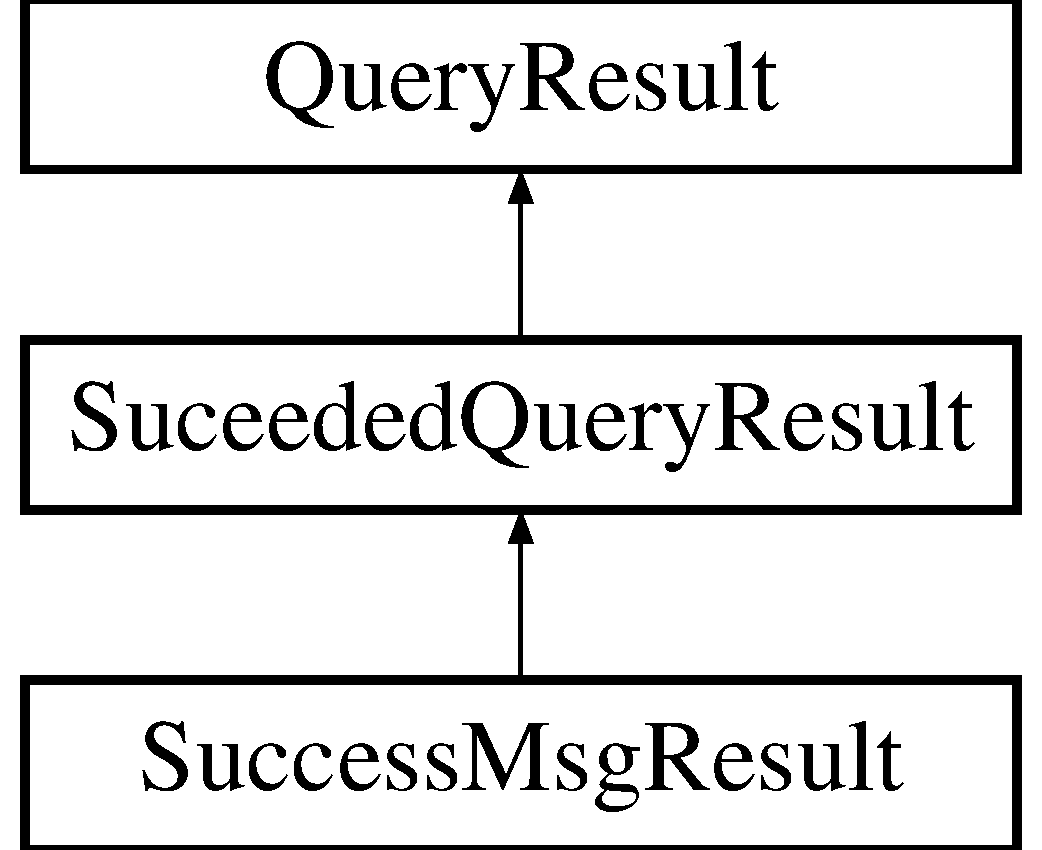
\includegraphics[height=3.000000cm]{class_success_msg_result}
\end{center}
\end{figure}
\subsection*{Public Member Functions}
\begin{DoxyCompactItemize}
\item 
\mbox{\Hypertarget{class_success_msg_result_a490473d12f70482f70ebb745862a3087}\label{class_success_msg_result_a490473d12f70482f70ebb745862a3087}} 
{\bfseries Success\+Msg\+Result} (const int number)
\item 
\mbox{\Hypertarget{class_success_msg_result_a56f5539bded5429768ea1b1b1071f43e}\label{class_success_msg_result_a56f5539bded5429768ea1b1b1071f43e}} 
{\bfseries Success\+Msg\+Result} (std\+::vector$<$ int $>$ results)
\item 
\mbox{\Hypertarget{class_success_msg_result_a502962f16dde2cfc7615c4fcc5492d2a}\label{class_success_msg_result_a502962f16dde2cfc7615c4fcc5492d2a}} 
{\bfseries Success\+Msg\+Result} (const char $\ast$qname)
\item 
\mbox{\Hypertarget{class_success_msg_result_ad64cc29af19b1bf721fb05e75190e0a1}\label{class_success_msg_result_ad64cc29af19b1bf721fb05e75190e0a1}} 
{\bfseries Success\+Msg\+Result} (const char $\ast$qname, const std\+::string \&msg)
\item 
\mbox{\Hypertarget{class_success_msg_result_aad32ebfe1de7a579d1292fcc47295e07}\label{class_success_msg_result_aad32ebfe1de7a579d1292fcc47295e07}} 
{\bfseries Success\+Msg\+Result} (const char $\ast$qname, const char $\ast$table, const std\+::string \&msg)
\item 
\mbox{\Hypertarget{class_success_msg_result_a97af69dd704091d77dcf48ca726690e3}\label{class_success_msg_result_a97af69dd704091d77dcf48ca726690e3}} 
std\+::string {\bfseries to\+String} () override
\end{DoxyCompactItemize}
\subsection*{Additional Inherited Members}


\subsection{Detailed Description}


Definition at line 60 of file query\+\_\+results.\+h.



The documentation for this class was generated from the following file\+:\begin{DoxyCompactItemize}
\item 
src/query\+\_\+results.\+h\end{DoxyCompactItemize}

\hypertarget{class_suceeded_query_result}{}\section{Suceeded\+Query\+Result Class Reference}
\label{class_suceeded_query_result}\index{Suceeded\+Query\+Result@{Suceeded\+Query\+Result}}
Inheritance diagram for Suceeded\+Query\+Result\+:\begin{figure}[H]
\begin{center}
\leavevmode
\includegraphics[height=2.285714cm]{class_suceeded_query_result}
\end{center}
\end{figure}
\subsection*{Public Member Functions}
\begin{DoxyCompactItemize}
\item 
\mbox{\Hypertarget{class_suceeded_query_result_a9080ba9ec97b32638efab6fa9472de94}\label{class_suceeded_query_result_a9080ba9ec97b32638efab6fa9472de94}} 
bool {\bfseries success} () override
\end{DoxyCompactItemize}
\subsection*{Additional Inherited Members}


\subsection{Detailed Description}


Definition at line 28 of file query\+\_\+results.\+h.



The documentation for this class was generated from the following file\+:\begin{DoxyCompactItemize}
\item 
src/query\+\_\+results.\+h\end{DoxyCompactItemize}

\hypertarget{class_sum_query}{}\section{Sum\+Query Class Reference}
\label{class_sum_query}\index{Sum\+Query@{Sum\+Query}}
Inheritance diagram for Sum\+Query\+:\begin{figure}[H]
\begin{center}
\leavevmode
\includegraphics[height=4.000000cm]{class_sum_query}
\end{center}
\end{figure}
\subsection*{Public Member Functions}
\begin{DoxyCompactItemize}
\item 
\mbox{\Hypertarget{class_sum_query_a9103b3e0edd89aaf08c87d765e07c69c}\label{class_sum_query_a9103b3e0edd89aaf08c87d765e07c69c}} 
{\bfseries L\+E\+M\+O\+N\+D\+B\+\_\+\+Q\+U\+E\+R\+Y\+\_\+\+W\+R\+I\+T\+ER} (false)
\item 
\mbox{\Hypertarget{class_sum_query_ae2b88c927e0d13a155863004e69185ad}\label{class_sum_query_ae2b88c927e0d13a155863004e69185ad}} 
Query\+Result\+::\+Ptr {\bfseries execute} () override
\item 
\mbox{\Hypertarget{class_sum_query_aa25cd7593520f1da60b6acfad4db5849}\label{class_sum_query_aa25cd7593520f1da60b6acfad4db5849}} 
std\+::string {\bfseries to\+String} () override
\item 
\mbox{\Hypertarget{class_sum_query_ac63c708b0d6a62f7124785ad041472f8}\label{class_sum_query_ac63c708b0d6a62f7124785ad041472f8}} 
Query\+Result\+::\+Ptr {\bfseries combine} (int \hyperlink{class_task_query_a3dc3e4c56ddea8ff025239fd9da358d3}{task\+Complete}) override
\end{DoxyCompactItemize}
\subsection*{Protected Member Functions}
\begin{DoxyCompactItemize}
\item 
\mbox{\Hypertarget{class_sum_query_a0db4bf7e9e2ae9a616891bcb07586344}\label{class_sum_query_a0db4bf7e9e2ae9a616891bcb07586344}} 
{\bfseries L\+E\+M\+O\+N\+D\+B\+\_\+\+T\+A\+S\+K\+\_\+\+P\+T\+R\+\_\+\+D\+EF} (\hyperlink{class_sum_task}{Sum\+Task})
\end{DoxyCompactItemize}
\subsection*{Friends}
\begin{DoxyCompactItemize}
\item 
\mbox{\Hypertarget{class_sum_query_a2bbe94890b2996fa2c9c59ecbb6021fb}\label{class_sum_query_a2bbe94890b2996fa2c9c59ecbb6021fb}} 
class {\bfseries Sum\+Task}
\end{DoxyCompactItemize}
\subsection*{Additional Inherited Members}


\subsection{Detailed Description}


Definition at line 13 of file sum\+\_\+query.\+h.



The documentation for this class was generated from the following files\+:\begin{DoxyCompactItemize}
\item 
src/query/data/sum\+\_\+query.\+h\item 
src/query/data/sum\+\_\+query.\+cpp\end{DoxyCompactItemize}

\hypertarget{class_sum_task}{}\section{Sum\+Task Class Reference}
\label{class_sum_task}\index{Sum\+Task@{Sum\+Task}}
Inheritance diagram for Sum\+Task\+:\begin{figure}[H]
\begin{center}
\leavevmode
\includegraphics[height=2.000000cm]{class_sum_task}
\end{center}
\end{figure}
\subsection*{Public Member Functions}
\begin{DoxyCompactItemize}
\item 
\mbox{\Hypertarget{class_sum_task_a9a1691dab970d420b7027ff50789d05f}\label{class_sum_task_a9a1691dab970d420b7027ff50789d05f}} 
void {\bfseries execute} () override
\end{DoxyCompactItemize}
\subsection*{Protected Member Functions}
\begin{DoxyCompactItemize}
\item 
\mbox{\Hypertarget{class_sum_task_ae505e938fc04421e69f614c8a81413eb}\label{class_sum_task_ae505e938fc04421e69f614c8a81413eb}} 
{\bfseries L\+E\+M\+O\+N\+D\+B\+\_\+\+Q\+U\+E\+R\+Y\+\_\+\+P\+TR} (\hyperlink{class_sum_query}{Sum\+Query})
\end{DoxyCompactItemize}
\subsection*{Friends}
\begin{DoxyCompactItemize}
\item 
\mbox{\Hypertarget{class_sum_task_ae1e90670d9f36a7b5dd14ff65c070805}\label{class_sum_task_ae1e90670d9f36a7b5dd14ff65c070805}} 
class {\bfseries Sum\+Query}
\end{DoxyCompactItemize}
\subsection*{Additional Inherited Members}


\subsection{Detailed Description}


Definition at line 27 of file sum\+\_\+query.\+h.



The documentation for this class was generated from the following files\+:\begin{DoxyCompactItemize}
\item 
src/query/data/sum\+\_\+query.\+h\item 
src/query/data/sum\+\_\+query.\+cpp\end{DoxyCompactItemize}

\hypertarget{class_swap_query}{}\section{Swap\+Query Class Reference}
\label{class_swap_query}\index{Swap\+Query@{Swap\+Query}}
Inheritance diagram for Swap\+Query\+:\begin{figure}[H]
\begin{center}
\leavevmode
\includegraphics[height=4.000000cm]{class_swap_query}
\end{center}
\end{figure}
\subsection*{Public Member Functions}
\begin{DoxyCompactItemize}
\item 
\mbox{\Hypertarget{class_swap_query_a7742c2e9fd7ce6fb450ac6e2b770ee64}\label{class_swap_query_a7742c2e9fd7ce6fb450ac6e2b770ee64}} 
{\bfseries L\+E\+M\+O\+N\+D\+B\+\_\+\+Q\+U\+E\+R\+Y\+\_\+\+W\+R\+I\+T\+ER} (true)
\item 
\mbox{\Hypertarget{class_swap_query_a70d41991d7e02d471adedc8d008e7725}\label{class_swap_query_a70d41991d7e02d471adedc8d008e7725}} 
Query\+Result\+::\+Ptr {\bfseries execute} () override
\item 
\mbox{\Hypertarget{class_swap_query_a2b125ce89dbc801b0167c045c8c25494}\label{class_swap_query_a2b125ce89dbc801b0167c045c8c25494}} 
std\+::string {\bfseries to\+String} () override
\item 
\mbox{\Hypertarget{class_swap_query_ae5131a8e6174ba815e2fac18fecae0f3}\label{class_swap_query_ae5131a8e6174ba815e2fac18fecae0f3}} 
Query\+Result\+::\+Ptr {\bfseries combine} (int \hyperlink{class_task_query_a3dc3e4c56ddea8ff025239fd9da358d3}{task\+Complete}) override
\end{DoxyCompactItemize}
\subsection*{Friends}
\begin{DoxyCompactItemize}
\item 
\mbox{\Hypertarget{class_swap_query_a1645be9f6c26c9fe1dfa5eaa6a2f98df}\label{class_swap_query_a1645be9f6c26c9fe1dfa5eaa6a2f98df}} 
class {\bfseries Swap\+Task}
\end{DoxyCompactItemize}
\subsection*{Additional Inherited Members}


\subsection{Detailed Description}


Definition at line 12 of file swap\+\_\+query.\+h.



The documentation for this class was generated from the following files\+:\begin{DoxyCompactItemize}
\item 
src/query/data/swap\+\_\+query.\+h\item 
src/query/data/swap\+\_\+query.\+cpp\end{DoxyCompactItemize}

\hypertarget{class_swap_task}{}\section{Swap\+Task Class Reference}
\label{class_swap_task}\index{Swap\+Task@{Swap\+Task}}
Inheritance diagram for Swap\+Task\+:\begin{figure}[H]
\begin{center}
\leavevmode
\includegraphics[height=2.000000cm]{class_swap_task}
\end{center}
\end{figure}
\subsection*{Public Member Functions}
\begin{DoxyCompactItemize}
\item 
\mbox{\Hypertarget{class_swap_task_a4316589196b4c497d759bcabbd891d27}\label{class_swap_task_a4316589196b4c497d759bcabbd891d27}} 
void {\bfseries execute} () override
\end{DoxyCompactItemize}
\subsection*{Protected Member Functions}
\begin{DoxyCompactItemize}
\item 
\mbox{\Hypertarget{class_swap_task_a4e90c55667d739be6a175bde0f472727}\label{class_swap_task_a4e90c55667d739be6a175bde0f472727}} 
{\bfseries L\+E\+M\+O\+N\+D\+B\+\_\+\+Q\+U\+E\+R\+Y\+\_\+\+P\+TR} (\hyperlink{class_swap_query}{Swap\+Query})
\end{DoxyCompactItemize}
\subsection*{Friends}
\begin{DoxyCompactItemize}
\item 
\mbox{\Hypertarget{class_swap_task_acc506341f1ba1e2a2c539110c8d1a525}\label{class_swap_task_acc506341f1ba1e2a2c539110c8d1a525}} 
class {\bfseries Swap\+Query}
\end{DoxyCompactItemize}
\subsection*{Additional Inherited Members}


\subsection{Detailed Description}


Definition at line 27 of file swap\+\_\+query.\+h.



The documentation for this class was generated from the following files\+:\begin{DoxyCompactItemize}
\item 
src/query/data/swap\+\_\+query.\+h\item 
src/query/data/swap\+\_\+query.\+cpp\end{DoxyCompactItemize}

\hypertarget{class_table}{}\section{Table Class Reference}
\label{class_table}\index{Table@{Table}}
\subsection*{Classes}
\begin{DoxyCompactItemize}
\item 
class \hyperlink{class_table_1_1_iterator_impl}{Iterator\+Impl}
\item 
class \hyperlink{class_table_1_1_object_impl}{Object\+Impl}
\end{DoxyCompactItemize}
\subsection*{Public Types}
\begin{DoxyCompactItemize}
\item 
\mbox{\Hypertarget{class_table_a7ec536bb39802e0f446dad42e08d4fdf}\label{class_table_a7ec536bb39802e0f446dad42e08d4fdf}} 
typedef std\+::string {\bfseries Key\+Type}
\item 
\mbox{\Hypertarget{class_table_a3535e31e3b4cb2fef2b18ff98657fa85}\label{class_table_a3535e31e3b4cb2fef2b18ff98657fa85}} 
typedef std\+::string {\bfseries Field\+Name\+Type}
\item 
\mbox{\Hypertarget{class_table_a3b5004cab41ef3fcf8708aefd44228b6}\label{class_table_a3b5004cab41ef3fcf8708aefd44228b6}} 
typedef size\+\_\+t {\bfseries Field\+Index}
\item 
\mbox{\Hypertarget{class_table_aaa438add915f9459416dab957f52ee63}\label{class_table_aaa438add915f9459416dab957f52ee63}} 
typedef int {\bfseries Value\+Type}
\item 
\mbox{\Hypertarget{class_table_af5796c55702b4b5e3eeb35670d9b242a}\label{class_table_af5796c55702b4b5e3eeb35670d9b242a}} 
typedef size\+\_\+t {\bfseries Size\+Type}
\item 
\mbox{\Hypertarget{class_table_a15892db3d57f25fafe199f593614ffdf}\label{class_table_a15892db3d57f25fafe199f593614ffdf}} 
typedef std\+::unique\+\_\+ptr$<$ \hyperlink{class_table}{Table} $>$ {\bfseries Ptr}
\item 
\mbox{\Hypertarget{class_table_a930877dd111fb5403afff7c400c25925}\label{class_table_a930877dd111fb5403afff7c400c25925}} 
typedef \hyperlink{class_table_1_1_object_impl}{Object\+Impl}$<$ Data\+Iterator, Value\+Type $>$ {\bfseries Object}
\item 
\mbox{\Hypertarget{class_table_adbcee28c19fcaa0904e71f2d76b80c31}\label{class_table_adbcee28c19fcaa0904e71f2d76b80c31}} 
typedef \hyperlink{class_table_1_1_object_impl}{Object\+Impl}$<$ Const\+Data\+Iterator, const Value\+Type $>$ {\bfseries Const\+Object}
\item 
\mbox{\Hypertarget{class_table_a41a3e845dfe45869c641cc564a70b328}\label{class_table_a41a3e845dfe45869c641cc564a70b328}} 
typedef \hyperlink{class_table_1_1_iterator_impl}{Iterator\+Impl}$<$ \hyperlink{class_table_1_1_object_impl}{Object}, decltype(data.\+begin())$>$ {\bfseries Iterator}
\item 
\mbox{\Hypertarget{class_table_a745f59742a52fe738da52323c23dbe29}\label{class_table_a745f59742a52fe738da52323c23dbe29}} 
typedef \hyperlink{class_table_1_1_iterator_impl}{Iterator\+Impl}$<$ \hyperlink{class_table_1_1_object_impl}{Const\+Object}, decltype(data.\+cbegin())$>$ {\bfseries Const\+Iterator}
\end{DoxyCompactItemize}
\subsection*{Public Member Functions}
\begin{DoxyCompactItemize}
\item 
\mbox{\Hypertarget{class_table_a875b5199dcecbdf2a2430856e4761d6b}\label{class_table_a875b5199dcecbdf2a2430856e4761d6b}} 
{\bfseries Table} (const std\+::string \&\hyperlink{class_table_aac2cc68c2c50c66f7de7656fa495fc2a}{name})
\item 
\mbox{\Hypertarget{class_table_aeb192735d371cc146836b7a4c1fe627c}\label{class_table_aeb192735d371cc146836b7a4c1fe627c}} 
{\footnotesize template$<$class Field\+I\+D\+Container $>$ }\\{\bfseries Table} (const std\+::string \&\hyperlink{class_table_aac2cc68c2c50c66f7de7656fa495fc2a}{name}, const Field\+I\+D\+Container \&\+\_\+fields)
\item 
\mbox{\Hypertarget{class_table_a56b5ff78a58e18398f8c36fac93b21d7}\label{class_table_a56b5ff78a58e18398f8c36fac93b21d7}} 
{\footnotesize template$<$class Field\+I\+D\+Container $>$ }\\void {\bfseries init} (const Field\+I\+D\+Container \&fields)
\item 
\mbox{\Hypertarget{class_table_a9efda1846fa5fe1e1c11e79896c26211}\label{class_table_a9efda1846fa5fe1e1c11e79896c26211}} 
{\bfseries Table} (std\+::string \hyperlink{class_table_aac2cc68c2c50c66f7de7656fa495fc2a}{name}, const \hyperlink{class_table}{Table} \&origin)
\item 
\mbox{\Hypertarget{class_table_a9d36a9931085cb0626c4c3361a5470b6}\label{class_table_a9d36a9931085cb0626c4c3361a5470b6}} 
void {\bfseries copy} (const \hyperlink{class_table}{Table} \&origin)
\item 
\mbox{\Hypertarget{class_table_a5b8b8c25efea1b8da70b223cf9829c1a}\label{class_table_a5b8b8c25efea1b8da70b223cf9829c1a}} 
void {\bfseries drop} ()
\item 
\mbox{\Hypertarget{class_table_ae2c8c050e99e9f85fd543a1768baa3a7}\label{class_table_ae2c8c050e99e9f85fd543a1768baa3a7}} 
bool {\bfseries is\+Inited} () const
\item 
\mbox{\Hypertarget{class_table_aa7527dfb6c0bf79d75dcb18e85fba8ff}\label{class_table_aa7527dfb6c0bf79d75dcb18e85fba8ff}} 
Field\+Index {\bfseries get\+Field\+Index} (const Field\+Name\+Type \&\hyperlink{class_table_ab68bc133d1d01f516d0bfb1a9c06e40f}{field}) const
\item 
\mbox{\Hypertarget{class_table_a4abc8b47696c07171b014c08c4df49b7}\label{class_table_a4abc8b47696c07171b014c08c4df49b7}} 
{\footnotesize template$<$class Value\+Type\+Container $>$ }\\void {\bfseries insert\+By\+Index} (Key\+Type key, const Value\+Type\+Container \&data)
\item 
Object\+::\+Ptr \hyperlink{class_table_a71ca4f3dfa88d0b057cd63920c5028e9}{operator\mbox{[}$\,$\mbox{]}} (const Key\+Type \&key)
\item 
void \hyperlink{class_table_ad0e71468c62bca660627296be71dc590}{erase\+Unique} (Object\+::\+Ptr \&\&object)
\item 
void \hyperlink{class_table_a9597c9976c3b83f757171f44c4101120}{erase} (const \hyperlink{class_table_1_1_iterator_impl}{Iterator} \&it)
\item 
void \hyperlink{class_table_a2c4dc9ae2d3c20e2b20fab04b996ccc4}{move} (\hyperlink{class_table_1_1_iterator_impl}{Iterator} \&it)
\item 
void \hyperlink{class_table_ae064a04cc7772a51f163f81f0187446e}{swap\+Data} ()
\item 
bool \hyperlink{class_table_aa7b2e954e0631acf5fbfe3e801eca1e3}{duplicate} (\hyperlink{class_table_1_1_iterator_impl}{Iterator} \&it)
\item 
void \hyperlink{class_table_a3b94156f321448e74ad74b0276ca1a32}{merge\+Data} ()
\item 
void \hyperlink{class_table_aaee2603a21e2ad0de4e073ada88e4b8d}{set\+Name} (std\+::string \hyperlink{class_table_aac2cc68c2c50c66f7de7656fa495fc2a}{name})
\item 
const std\+::string \& \hyperlink{class_table_aac2cc68c2c50c66f7de7656fa495fc2a}{name} () const
\item 
bool \hyperlink{class_table_abb7690114d028b87e337540f42780cbb}{empty} () const
\item 
size\+\_\+t \hyperlink{class_table_aec548eba07f9b3aebcde324c19e19fde}{size} () const
\item 
const std\+::vector$<$ Field\+Name\+Type $>$ \& \hyperlink{class_table_ab68bc133d1d01f516d0bfb1a9c06e40f}{field} () const
\item 
size\+\_\+t \hyperlink{class_table_af94164c4dde76690be6b7f3a1d5e7733}{clear} ()
\item 
\hyperlink{class_table_1_1_iterator_impl}{Iterator} \hyperlink{class_table_a9df56e33923bbff648f98367d723ddb5}{begin} ()
\item 
\hyperlink{class_table_1_1_iterator_impl}{Iterator} \hyperlink{class_table_a5b5c1e536a44af329e2a9e35e469fde7}{end} ()
\item 
\hyperlink{class_table_1_1_iterator_impl}{Const\+Iterator} \hyperlink{class_table_a8b9f35b26e064b9104afcdc804e05883}{begin} () const
\item 
\hyperlink{class_table_1_1_iterator_impl}{Const\+Iterator} \hyperlink{class_table_a7fa70114351a55ad1602f48396d13359}{end} () const
\item 
\mbox{\Hypertarget{class_table_a7a5b44db06f077bea635ce5c0c24f0bf}\label{class_table_a7a5b44db06f077bea635ce5c0c24f0bf}} 
void {\bfseries add\+Query} (\hyperlink{class_query}{Query} $\ast$query)
\item 
\mbox{\Hypertarget{class_table_a2a88ee4aa176f0763b90bc71a82813a8}\label{class_table_a2a88ee4aa176f0763b90bc71a82813a8}} 
void {\bfseries complete\+Query} ()
\end{DoxyCompactItemize}
\subsection*{Static Public Attributes}
\begin{DoxyCompactItemize}
\item 
\mbox{\Hypertarget{class_table_a18c1c0fc4538dcd9c38b66afa63b1739}\label{class_table_a18c1c0fc4538dcd9c38b66afa63b1739}} 
static constexpr const Value\+Type {\bfseries Value\+Type\+Max} = I\+N\+T32\+\_\+\+M\+AX
\item 
\mbox{\Hypertarget{class_table_a91fea5fb967510c0c6e66efff8c39f7d}\label{class_table_a91fea5fb967510c0c6e66efff8c39f7d}} 
static constexpr const Value\+Type {\bfseries Value\+Type\+Min} = I\+N\+T32\+\_\+\+M\+IN
\end{DoxyCompactItemize}
\subsection*{Friends}
\begin{DoxyCompactItemize}
\item 
std\+::ostream \& \hyperlink{class_table_ac91202688e17b1c145b7d98d90ace349}{operator$<$$<$} (std\+::ostream \&os, const \hyperlink{class_table}{Table} \&table)
\end{DoxyCompactItemize}


\subsection{Detailed Description}


Definition at line 50 of file db\+\_\+table.\+h.



\subsection{Member Function Documentation}
\mbox{\Hypertarget{class_table_a9df56e33923bbff648f98367d723ddb5}\label{class_table_a9df56e33923bbff648f98367d723ddb5}} 
\index{Table@{Table}!begin@{begin}}
\index{begin@{begin}!Table@{Table}}
\subsubsection{\texorpdfstring{begin()}{begin()}\hspace{0.1cm}{\footnotesize\ttfamily [1/2]}}
{\footnotesize\ttfamily \hyperlink{class_table_1_1_iterator_impl}{Iterator} Table\+::begin (\begin{DoxyParamCaption}{ }\end{DoxyParamCaption})\hspace{0.3cm}{\ttfamily [inline]}}

Get a begin iterator similar to the standard iterator \begin{DoxyReturn}{Returns}
begin iterator 
\end{DoxyReturn}


Definition at line 474 of file db\+\_\+table.\+h.

\mbox{\Hypertarget{class_table_a8b9f35b26e064b9104afcdc804e05883}\label{class_table_a8b9f35b26e064b9104afcdc804e05883}} 
\index{Table@{Table}!begin@{begin}}
\index{begin@{begin}!Table@{Table}}
\subsubsection{\texorpdfstring{begin()}{begin()}\hspace{0.1cm}{\footnotesize\ttfamily [2/2]}}
{\footnotesize\ttfamily \hyperlink{class_table_1_1_iterator_impl}{Const\+Iterator} Table\+::begin (\begin{DoxyParamCaption}{ }\end{DoxyParamCaption}) const\hspace{0.3cm}{\ttfamily [inline]}}

Get a const begin iterator similar to the standard iterator \begin{DoxyReturn}{Returns}
const begin iterator 
\end{DoxyReturn}


Definition at line 486 of file db\+\_\+table.\+h.

\mbox{\Hypertarget{class_table_af94164c4dde76690be6b7f3a1d5e7733}\label{class_table_af94164c4dde76690be6b7f3a1d5e7733}} 
\index{Table@{Table}!clear@{clear}}
\index{clear@{clear}!Table@{Table}}
\subsubsection{\texorpdfstring{clear()}{clear()}}
{\footnotesize\ttfamily size\+\_\+t Table\+::clear (\begin{DoxyParamCaption}{ }\end{DoxyParamCaption})\hspace{0.3cm}{\ttfamily [inline]}}

Clear all content in the table \begin{DoxyReturn}{Returns}
rows affected 
\end{DoxyReturn}


Definition at line 463 of file db\+\_\+table.\+h.

\mbox{\Hypertarget{class_table_aa7b2e954e0631acf5fbfe3e801eca1e3}\label{class_table_aa7b2e954e0631acf5fbfe3e801eca1e3}} 
\index{Table@{Table}!duplicate@{duplicate}}
\index{duplicate@{duplicate}!Table@{Table}}
\subsubsection{\texorpdfstring{duplicate()}{duplicate()}}
{\footnotesize\ttfamily bool Table\+::duplicate (\begin{DoxyParamCaption}\item[{\hyperlink{class_table_1_1_iterator_impl}{Iterator} \&}]{it }\end{DoxyParamCaption})\hspace{0.3cm}{\ttfamily [inline]}}

Duplicate it and put it into data\+New if \{key\}\+\_\+copy exists, nothing happens this function is used only in duplicate query 

Definition at line 404 of file db\+\_\+table.\+h.

\mbox{\Hypertarget{class_table_abb7690114d028b87e337540f42780cbb}\label{class_table_abb7690114d028b87e337540f42780cbb}} 
\index{Table@{Table}!empty@{empty}}
\index{empty@{empty}!Table@{Table}}
\subsubsection{\texorpdfstring{empty()}{empty()}}
{\footnotesize\ttfamily bool Table\+::empty (\begin{DoxyParamCaption}{ }\end{DoxyParamCaption}) const\hspace{0.3cm}{\ttfamily [inline]}}

Return whether the table is empty \begin{DoxyReturn}{Returns}

\end{DoxyReturn}


Definition at line 445 of file db\+\_\+table.\+h.

\mbox{\Hypertarget{class_table_a5b5c1e536a44af329e2a9e35e469fde7}\label{class_table_a5b5c1e536a44af329e2a9e35e469fde7}} 
\index{Table@{Table}!end@{end}}
\index{end@{end}!Table@{Table}}
\subsubsection{\texorpdfstring{end()}{end()}\hspace{0.1cm}{\footnotesize\ttfamily [1/2]}}
{\footnotesize\ttfamily \hyperlink{class_table_1_1_iterator_impl}{Iterator} Table\+::end (\begin{DoxyParamCaption}{ }\end{DoxyParamCaption})\hspace{0.3cm}{\ttfamily [inline]}}

Get a end iterator similar to the standard iterator \begin{DoxyReturn}{Returns}
end iterator 
\end{DoxyReturn}


Definition at line 480 of file db\+\_\+table.\+h.

\mbox{\Hypertarget{class_table_a7fa70114351a55ad1602f48396d13359}\label{class_table_a7fa70114351a55ad1602f48396d13359}} 
\index{Table@{Table}!end@{end}}
\index{end@{end}!Table@{Table}}
\subsubsection{\texorpdfstring{end()}{end()}\hspace{0.1cm}{\footnotesize\ttfamily [2/2]}}
{\footnotesize\ttfamily \hyperlink{class_table_1_1_iterator_impl}{Const\+Iterator} Table\+::end (\begin{DoxyParamCaption}{ }\end{DoxyParamCaption}) const\hspace{0.3cm}{\ttfamily [inline]}}

Get a const end iterator similar to the standard iterator \begin{DoxyReturn}{Returns}
const end iterator 
\end{DoxyReturn}


Definition at line 492 of file db\+\_\+table.\+h.

\mbox{\Hypertarget{class_table_a9597c9976c3b83f757171f44c4101120}\label{class_table_a9597c9976c3b83f757171f44c4101120}} 
\index{Table@{Table}!erase@{erase}}
\index{erase@{erase}!Table@{Table}}
\subsubsection{\texorpdfstring{erase()}{erase()}}
{\footnotesize\ttfamily void Table\+::erase (\begin{DoxyParamCaption}\item[{const \hyperlink{class_table_1_1_iterator_impl}{Iterator} \&}]{it }\end{DoxyParamCaption})\hspace{0.3cm}{\ttfamily [inline]}}

thread safe function Erase the key in the table Caution\+: this function only erases the key in key\+Map, leaves data unchanged no other operation related to key\+Map can be applied before swap\+Data is called 
\begin{DoxyParams}{Parameters}
{\em it} & \\
\hline
\end{DoxyParams}


Definition at line 368 of file db\+\_\+table.\+h.

\mbox{\Hypertarget{class_table_ad0e71468c62bca660627296be71dc590}\label{class_table_ad0e71468c62bca660627296be71dc590}} 
\index{Table@{Table}!erase\+Unique@{erase\+Unique}}
\index{erase\+Unique@{erase\+Unique}!Table@{Table}}
\subsubsection{\texorpdfstring{erase\+Unique()}{eraseUnique()}}
{\footnotesize\ttfamily void Table\+::erase\+Unique (\begin{DoxyParamCaption}\item[{Object\+::\+Ptr \&\&}]{object }\end{DoxyParamCaption})\hspace{0.3cm}{\ttfamily [inline]}}

not thread safe function Remove only one datum only used when delete by key 
\begin{DoxyParams}{Parameters}
{\em it} & \\
\hline
\end{DoxyParams}


Definition at line 355 of file db\+\_\+table.\+h.

\mbox{\Hypertarget{class_table_ab68bc133d1d01f516d0bfb1a9c06e40f}\label{class_table_ab68bc133d1d01f516d0bfb1a9c06e40f}} 
\index{Table@{Table}!field@{field}}
\index{field@{field}!Table@{Table}}
\subsubsection{\texorpdfstring{field()}{field()}}
{\footnotesize\ttfamily const std\+::vector$<$Field\+Name\+Type$>$\& Table\+::field (\begin{DoxyParamCaption}{ }\end{DoxyParamCaption}) const\hspace{0.3cm}{\ttfamily [inline]}}

Return the fields in the table \begin{DoxyReturn}{Returns}

\end{DoxyReturn}


Definition at line 457 of file db\+\_\+table.\+h.

\mbox{\Hypertarget{class_table_a3b94156f321448e74ad74b0276ca1a32}\label{class_table_a3b94156f321448e74ad74b0276ca1a32}} 
\index{Table@{Table}!merge\+Data@{merge\+Data}}
\index{merge\+Data@{merge\+Data}!Table@{Table}}
\subsubsection{\texorpdfstring{merge\+Data()}{mergeData()}}
{\footnotesize\ttfamily void Table\+::merge\+Data (\begin{DoxyParamCaption}{ }\end{DoxyParamCaption})\hspace{0.3cm}{\ttfamily [inline]}}

insert data\+New to the end of data then data\+New is cleared for future query this function is used only in duplicate query 

Definition at line 421 of file db\+\_\+table.\+h.

\mbox{\Hypertarget{class_table_a2c4dc9ae2d3c20e2b20fab04b996ccc4}\label{class_table_a2c4dc9ae2d3c20e2b20fab04b996ccc4}} 
\index{Table@{Table}!move@{move}}
\index{move@{move}!Table@{Table}}
\subsubsection{\texorpdfstring{move()}{move()}}
{\footnotesize\ttfamily void Table\+::move (\begin{DoxyParamCaption}\item[{\hyperlink{class_table_1_1_iterator_impl}{Iterator} \&}]{it }\end{DoxyParamCaption})\hspace{0.3cm}{\ttfamily [inline]}}

thread safe function Move datum from data to data\+New Caution\+: iterator it can\textquotesingle{}t be accessed again after \hyperlink{class_table_a2c4dc9ae2d3c20e2b20fab04b996ccc4}{move()} is called no other operation related to key\+Map can be applied before swap\+Data is called 
\begin{DoxyParams}{Parameters}
{\em it} & \\
\hline
\end{DoxyParams}


Definition at line 381 of file db\+\_\+table.\+h.

\mbox{\Hypertarget{class_table_aac2cc68c2c50c66f7de7656fa495fc2a}\label{class_table_aac2cc68c2c50c66f7de7656fa495fc2a}} 
\index{Table@{Table}!name@{name}}
\index{name@{name}!Table@{Table}}
\subsubsection{\texorpdfstring{name()}{name()}}
{\footnotesize\ttfamily const std\+::string\& Table\+::name (\begin{DoxyParamCaption}{ }\end{DoxyParamCaption}) const\hspace{0.3cm}{\ttfamily [inline]}}

Get the name of the table \begin{DoxyReturn}{Returns}

\end{DoxyReturn}


Definition at line 439 of file db\+\_\+table.\+h.

\mbox{\Hypertarget{class_table_a71ca4f3dfa88d0b057cd63920c5028e9}\label{class_table_a71ca4f3dfa88d0b057cd63920c5028e9}} 
\index{Table@{Table}!operator\mbox{[}\mbox{]}@{operator[]}}
\index{operator\mbox{[}\mbox{]}@{operator[]}!Table@{Table}}
\subsubsection{\texorpdfstring{operator[]()}{operator[]()}}
{\footnotesize\ttfamily Object\+::\+Ptr Table\+::operator\mbox{[}$\,$\mbox{]} (\begin{DoxyParamCaption}\item[{const Key\+Type \&}]{key }\end{DoxyParamCaption})\hspace{0.3cm}{\ttfamily [inline]}}

Access the value according to the key 
\begin{DoxyParams}{Parameters}
{\em key} & \\
\hline
\end{DoxyParams}
\begin{DoxyReturn}{Returns}
the Object that K\+EY = key, or nullptr if key doesn\textquotesingle{}t exist 
\end{DoxyReturn}


Definition at line 339 of file db\+\_\+table.\+h.

\mbox{\Hypertarget{class_table_aaee2603a21e2ad0de4e073ada88e4b8d}\label{class_table_aaee2603a21e2ad0de4e073ada88e4b8d}} 
\index{Table@{Table}!set\+Name@{set\+Name}}
\index{set\+Name@{set\+Name}!Table@{Table}}
\subsubsection{\texorpdfstring{set\+Name()}{setName()}}
{\footnotesize\ttfamily void Table\+::set\+Name (\begin{DoxyParamCaption}\item[{std\+::string}]{name }\end{DoxyParamCaption})\hspace{0.3cm}{\ttfamily [inline]}}

Set the name of the table 
\begin{DoxyParams}{Parameters}
{\em name} & \\
\hline
\end{DoxyParams}


Definition at line 433 of file db\+\_\+table.\+h.

\mbox{\Hypertarget{class_table_aec548eba07f9b3aebcde324c19e19fde}\label{class_table_aec548eba07f9b3aebcde324c19e19fde}} 
\index{Table@{Table}!size@{size}}
\index{size@{size}!Table@{Table}}
\subsubsection{\texorpdfstring{size()}{size()}}
{\footnotesize\ttfamily size\+\_\+t Table\+::size (\begin{DoxyParamCaption}{ }\end{DoxyParamCaption}) const\hspace{0.3cm}{\ttfamily [inline]}}

Return the num of data stored in the table \begin{DoxyReturn}{Returns}

\end{DoxyReturn}


Definition at line 451 of file db\+\_\+table.\+h.

\mbox{\Hypertarget{class_table_ae064a04cc7772a51f163f81f0187446e}\label{class_table_ae064a04cc7772a51f163f81f0187446e}} 
\index{Table@{Table}!swap\+Data@{swap\+Data}}
\index{swap\+Data@{swap\+Data}!Table@{Table}}
\subsubsection{\texorpdfstring{swap\+Data()}{swapData()}}
{\footnotesize\ttfamily void Table\+::swap\+Data (\begin{DoxyParamCaption}{ }\end{DoxyParamCaption})\hspace{0.3cm}{\ttfamily [inline]}}

not thread safe function Swap data and new\+Data vector\+::clear ensures that the capacity of data\+New unchanged so push\+\_\+back to data\+New is efficient 

Definition at line 394 of file db\+\_\+table.\+h.



\subsection{Friends And Related Function Documentation}
\mbox{\Hypertarget{class_table_ac91202688e17b1c145b7d98d90ace349}\label{class_table_ac91202688e17b1c145b7d98d90ace349}} 
\index{Table@{Table}!operator$<$$<$@{operator$<$$<$}}
\index{operator$<$$<$@{operator$<$$<$}!Table@{Table}}
\subsubsection{\texorpdfstring{operator$<$$<$}{operator<<}}
{\footnotesize\ttfamily std\+::ostream\& operator$<$$<$ (\begin{DoxyParamCaption}\item[{std\+::ostream \&}]{os,  }\item[{const \hyperlink{class_table}{Table} \&}]{table }\end{DoxyParamCaption})\hspace{0.3cm}{\ttfamily [friend]}}

Overload the $<$$<$ operator for complete print of the table 
\begin{DoxyParams}{Parameters}
{\em os} & \\
\hline
{\em table} & \\
\hline
\end{DoxyParams}
\begin{DoxyReturn}{Returns}
the origin ostream 
\end{DoxyReturn}


Definition at line 94 of file db\+\_\+table.\+cpp.



The documentation for this class was generated from the following files\+:\begin{DoxyCompactItemize}
\item 
src/db/db\+\_\+table.\+h\item 
src/db/db\+\_\+table.\+cpp\end{DoxyCompactItemize}

\hypertarget{struct_table_field_not_found}{}\section{Table\+Field\+Not\+Found Struct Reference}
\label{struct_table_field_not_found}\index{Table\+Field\+Not\+Found@{Table\+Field\+Not\+Found}}
Inheritance diagram for Table\+Field\+Not\+Found\+:\begin{figure}[H]
\begin{center}
\leavevmode
\includegraphics[height=2.000000cm]{struct_table_field_not_found}
\end{center}
\end{figure}
\subsection*{Public Member Functions}
\begin{DoxyCompactItemize}
\item 
\mbox{\Hypertarget{struct_table_field_not_found_ae169abce20c581f32430e2a64b8471b4}\label{struct_table_field_not_found_ae169abce20c581f32430e2a64b8471b4}} 
{\bfseries Table\+Field\+Not\+Found} (const std\+::string \&str)
\end{DoxyCompactItemize}


\subsection{Detailed Description}


Definition at line 36 of file uexception.\+h.



The documentation for this struct was generated from the following file\+:\begin{DoxyCompactItemize}
\item 
src/uexception.\+h\end{DoxyCompactItemize}

\hypertarget{struct_table_name_not_found}{}\section{Table\+Name\+Not\+Found Struct Reference}
\label{struct_table_name_not_found}\index{Table\+Name\+Not\+Found@{Table\+Name\+Not\+Found}}
Inheritance diagram for Table\+Name\+Not\+Found\+:\begin{figure}[H]
\begin{center}
\leavevmode
\includegraphics[height=2.000000cm]{struct_table_name_not_found}
\end{center}
\end{figure}
\subsection*{Public Member Functions}
\begin{DoxyCompactItemize}
\item 
\mbox{\Hypertarget{struct_table_name_not_found_a19ad1a2f613641a309e7850db10f34aa}\label{struct_table_name_not_found_a19ad1a2f613641a309e7850db10f34aa}} 
{\bfseries Table\+Name\+Not\+Found} (const std\+::string \&str)
\end{DoxyCompactItemize}


\subsection{Detailed Description}


Definition at line 21 of file uexception.\+h.



The documentation for this struct was generated from the following file\+:\begin{DoxyCompactItemize}
\item 
src/uexception.\+h\end{DoxyCompactItemize}

\hypertarget{class_task}{}\section{Task Class Reference}
\label{class_task}\index{Task@{Task}}
Inheritance diagram for Task\+:\begin{figure}[H]
\begin{center}
\leavevmode
\includegraphics[height=12.000000cm]{class_task}
\end{center}
\end{figure}
\subsection*{Public Types}
\begin{DoxyCompactItemize}
\item 
\mbox{\Hypertarget{class_task_a636a488a23020fcac3380e0fc876e55c}\label{class_task_a636a488a23020fcac3380e0fc876e55c}} 
typedef std\+::unique\+\_\+ptr$<$ \hyperlink{class_task}{Task} $>$ {\bfseries Ptr}
\end{DoxyCompactItemize}
\subsection*{Public Member Functions}
\begin{DoxyCompactItemize}
\item 
\mbox{\Hypertarget{class_task_af0449cba22c5a93fea99a5cb100a24e9}\label{class_task_af0449cba22c5a93fea99a5cb100a24e9}} 
{\bfseries Task} (\hyperlink{class_query}{Query} $\ast$query, \hyperlink{class_table}{Table} $\ast$table=nullptr)
\item 
\mbox{\Hypertarget{class_task_aa42dbfc5b52058cdc161d7a8b7b023bf}\label{class_task_aa42dbfc5b52058cdc161d7a8b7b023bf}} 
{\bfseries Task} (\hyperlink{class_query}{Query} $\ast$query, \hyperlink{class_table}{Table} $\ast$table, \hyperlink{class_table_1_1_iterator_impl}{Table\+::\+Iterator} begin, \hyperlink{class_table_1_1_iterator_impl}{Table\+::\+Iterator} end)
\item 
\mbox{\Hypertarget{class_task_ade38031c3ed134ec20cbbcd58e575745}\label{class_task_ade38031c3ed134ec20cbbcd58e575745}} 
virtual void {\bfseries execute} ()
\item 
\mbox{\Hypertarget{class_task_a2b5770928a7e40b46ec339d67f747b32}\label{class_task_a2b5770928a7e40b46ec339d67f747b32}} 
Table\+::\+Size\+Type {\bfseries get\+Counter} () const
\end{DoxyCompactItemize}
\subsection*{Protected Member Functions}
\begin{DoxyCompactItemize}
\item 
\mbox{\Hypertarget{class_task_a755ffdd69b2a9e69afa239a7cf5bb768}\label{class_task_a755ffdd69b2a9e69afa239a7cf5bb768}} 
virtual \hyperlink{class_task_query}{Task\+Query} $\ast$ {\bfseries get\+Query} () const
\end{DoxyCompactItemize}
\subsection*{Protected Attributes}
\begin{DoxyCompactItemize}
\item 
\mbox{\Hypertarget{class_task_aba7c96b09298eb1d88c0cfba899a5370}\label{class_task_aba7c96b09298eb1d88c0cfba899a5370}} 
\hyperlink{class_query}{Query} $\ast$ {\bfseries query}
\item 
\mbox{\Hypertarget{class_task_a19f21bd1d9c8b2cc7e91b4cef04f0566}\label{class_task_a19f21bd1d9c8b2cc7e91b4cef04f0566}} 
\hyperlink{class_table}{Table} $\ast$ {\bfseries table} = nullptr
\item 
Table\+::\+Size\+Type \hyperlink{class_task_a797775a347a221efdaefe853a0977991}{counter} = 0
\item 
\mbox{\Hypertarget{class_task_ad33a49bbc4669f3293aa33c96dc79be1}\label{class_task_ad33a49bbc4669f3293aa33c96dc79be1}} 
\hyperlink{class_table_1_1_iterator_impl}{Table\+::\+Iterator} {\bfseries begin}
\item 
\mbox{\Hypertarget{class_task_a65eeb1f03bdfdbc3f98c69daf652a2e0}\label{class_task_a65eeb1f03bdfdbc3f98c69daf652a2e0}} 
\hyperlink{class_table_1_1_iterator_impl}{Table\+::\+Iterator} {\bfseries end}
\item 
\mbox{\Hypertarget{class_task_a42637d575d28f22528a8d90ed6c7bbe3}\label{class_task_a42637d575d28f22528a8d90ed6c7bbe3}} 
Query\+Result\+::\+Ptr {\bfseries error\+Result} = nullptr
\end{DoxyCompactItemize}
\subsection*{Friends}
\begin{DoxyCompactItemize}
\item 
\mbox{\Hypertarget{class_task_a6efef52d7a939622bbc934ff6b90ffe0}\label{class_task_a6efef52d7a939622bbc934ff6b90ffe0}} 
class {\bfseries Database}
\end{DoxyCompactItemize}


\subsection{Detailed Description}


Definition at line 12 of file task.\+h.



\subsection{Member Data Documentation}
\mbox{\Hypertarget{class_task_a797775a347a221efdaefe853a0977991}\label{class_task_a797775a347a221efdaefe853a0977991}} 
\index{Task@{Task}!counter@{counter}}
\index{counter@{counter}!Task@{Task}}
\subsubsection{\texorpdfstring{counter}{counter}}
{\footnotesize\ttfamily Table\+::\+Size\+Type Task\+::counter = 0\hspace{0.3cm}{\ttfamily [protected]}}

Count affected rows in this task 

Definition at line 17 of file task.\+h.



The documentation for this class was generated from the following files\+:\begin{DoxyCompactItemize}
\item 
src/query/task.\+h\item 
src/query/task.\+cpp\end{DoxyCompactItemize}

\hypertarget{class_task_query}{}\section{Task\+Query Class Reference}
\label{class_task_query}\index{Task\+Query@{Task\+Query}}
Inheritance diagram for Task\+Query\+:\begin{figure}[H]
\begin{center}
\leavevmode
\includegraphics[height=10.000000cm]{class_task_query}
\end{center}
\end{figure}
\subsection*{Public Member Functions}
\begin{DoxyCompactItemize}
\item 
\mbox{\Hypertarget{class_task_query_a07799ce7089a4a84062b5e5813706425}\label{class_task_query_a07799ce7089a4a84062b5e5813706425}} 
{\bfseries Task\+Query} (std\+::string target\+Table)
\item 
\mbox{\Hypertarget{class_task_query_af216a94f17cb6b35a534947cb4ef9892}\label{class_task_query_af216a94f17cb6b35a534947cb4ef9892}} 
\hyperlink{class_task}{Task} $\ast$ {\bfseries get\+Task} (size\+\_\+t index) const
\item 
\mbox{\Hypertarget{class_task_query_ac5990fbd75ae30962dd7ef1369571889}\label{class_task_query_ac5990fbd75ae30962dd7ef1369571889}} 
\hyperlink{class_task}{Task} $\ast$ {\bfseries get\+Task} (const std\+::vector$<$ std\+::unique\+\_\+ptr$<$ \hyperlink{class_task}{Task} $>$ $>$\+::iterator \&it) const
\item 
void \hyperlink{class_task_query_ad34220bba4a3fab50e5f59f63d7cf5e2}{start} ()
\item 
void \hyperlink{class_task_query_ab77bfd5f991d0cc596592966d3ed6193}{complete} ()
\item 
void \hyperlink{class_task_query_a91f0bc0a82e23db824e3ae6052026def}{complete} (Query\+Result\+::\+Ptr \&\&result)
\item 
{\footnotesize template$<$class Task\+Type $>$ }\\void \hyperlink{class_task_query_a9432212e101b6b393c13cf93e1211755}{add\+Iteration\+Task} (\hyperlink{class_database}{Database} \&db, \hyperlink{class_table}{Table} \&table)
\item 
{\footnotesize template$<$class Task\+Type $>$ }\\void \hyperlink{class_task_query_afb2a8505209d5f521570305f60203b2d}{add\+Unique\+Task} (\hyperlink{class_database}{Database} \&db, \hyperlink{class_table}{Table} $\ast$table=nullptr)
\end{DoxyCompactItemize}
\subsection*{Protected Attributes}
\begin{DoxyCompactItemize}
\item 
size\+\_\+t \hyperlink{class_task_query_a712ef51749dfd08ecdf6a33acaf6da4f}{tasks\+Size} = 1
\item 
int \hyperlink{class_task_query_a3dc3e4c56ddea8ff025239fd9da358d3}{task\+Complete} = 0
\item 
std\+::vector$<$ std\+::unique\+\_\+ptr$<$ \hyperlink{class_task}{Task} $>$ $>$ \hyperlink{class_task_query_a99c16ac776e6067ba79303396d398819}{tasks}
\item 
std\+::mutex \hyperlink{class_task_query_a147de82af025117cf5ae362dd4d75778}{tasks\+Mutex}
\end{DoxyCompactItemize}
\subsection*{Additional Inherited Members}


\subsection{Detailed Description}


Definition at line 33 of file query.\+h.



\subsection{Member Function Documentation}
\mbox{\Hypertarget{class_task_query_a9432212e101b6b393c13cf93e1211755}\label{class_task_query_a9432212e101b6b393c13cf93e1211755}} 
\index{Task\+Query@{Task\+Query}!add\+Iteration\+Task@{add\+Iteration\+Task}}
\index{add\+Iteration\+Task@{add\+Iteration\+Task}!Task\+Query@{Task\+Query}}
\subsubsection{\texorpdfstring{add\+Iteration\+Task()}{addIterationTask()}}
{\footnotesize\ttfamily template$<$class Task\+Type $>$ \\
void Task\+Query\+::add\+Iteration\+Task (\begin{DoxyParamCaption}\item[{\hyperlink{class_database}{Database} \&}]{db,  }\item[{\hyperlink{class_table}{Table} \&}]{table }\end{DoxyParamCaption})\hspace{0.3cm}{\ttfamily [inline]}}

For iteration query, we can split them in this function 

Definition at line 59 of file query.\+h.

\mbox{\Hypertarget{class_task_query_afb2a8505209d5f521570305f60203b2d}\label{class_task_query_afb2a8505209d5f521570305f60203b2d}} 
\index{Task\+Query@{Task\+Query}!add\+Unique\+Task@{add\+Unique\+Task}}
\index{add\+Unique\+Task@{add\+Unique\+Task}!Task\+Query@{Task\+Query}}
\subsubsection{\texorpdfstring{add\+Unique\+Task()}{addUniqueTask()}}
{\footnotesize\ttfamily template$<$class Task\+Type $>$ \\
void Task\+Query\+::add\+Unique\+Task (\begin{DoxyParamCaption}\item[{\hyperlink{class_database}{Database} \&}]{db,  }\item[{\hyperlink{class_table}{Table} $\ast$}]{table = {\ttfamily nullptr} }\end{DoxyParamCaption})\hspace{0.3cm}{\ttfamily [inline]}}

For non-\/iteration query that should be done later 

Definition at line 92 of file query.\+h.

\mbox{\Hypertarget{class_task_query_ab77bfd5f991d0cc596592966d3ed6193}\label{class_task_query_ab77bfd5f991d0cc596592966d3ed6193}} 
\index{Task\+Query@{Task\+Query}!complete@{complete}}
\index{complete@{complete}!Task\+Query@{Task\+Query}}
\subsubsection{\texorpdfstring{complete()}{complete()}\hspace{0.1cm}{\footnotesize\ttfamily [1/2]}}
{\footnotesize\ttfamily void Task\+Query\+::complete (\begin{DoxyParamCaption}{ }\end{DoxyParamCaption})}

Complete a task add the complete query to the result vector here should add a unique id for each query -\/ ok should add a function to print results in correct order

Definition at line 12 of file query.\+cpp.

\mbox{\Hypertarget{class_task_query_a91f0bc0a82e23db824e3ae6052026def}\label{class_task_query_a91f0bc0a82e23db824e3ae6052026def}} 
\index{Task\+Query@{Task\+Query}!complete@{complete}}
\index{complete@{complete}!Task\+Query@{Task\+Query}}
\subsubsection{\texorpdfstring{complete()}{complete()}\hspace{0.1cm}{\footnotesize\ttfamily [2/2]}}
{\footnotesize\ttfamily void Task\+Query\+::complete (\begin{DoxyParamCaption}\item[{Query\+Result\+::\+Ptr \&\&}]{result }\end{DoxyParamCaption})}

Complete a query 

Definition at line 26 of file query.\+cpp.

\mbox{\Hypertarget{class_task_query_ad34220bba4a3fab50e5f59f63d7cf5e2}\label{class_task_query_ad34220bba4a3fab50e5f59f63d7cf5e2}} 
\index{Task\+Query@{Task\+Query}!start@{start}}
\index{start@{start}!Task\+Query@{Task\+Query}}
\subsubsection{\texorpdfstring{start()}{start()}}
{\footnotesize\ttfamily void Task\+Query\+::start (\begin{DoxyParamCaption}{ }\end{DoxyParamCaption})}

Debug function for starting a query 

Definition at line 8 of file query.\+cpp.



\subsection{Member Data Documentation}
\mbox{\Hypertarget{class_task_query_a3dc3e4c56ddea8ff025239fd9da358d3}\label{class_task_query_a3dc3e4c56ddea8ff025239fd9da358d3}} 
\index{Task\+Query@{Task\+Query}!task\+Complete@{task\+Complete}}
\index{task\+Complete@{task\+Complete}!Task\+Query@{Task\+Query}}
\subsubsection{\texorpdfstring{task\+Complete}{taskComplete}}
{\footnotesize\ttfamily int Task\+Query\+::task\+Complete = 0\hspace{0.3cm}{\ttfamily [protected]}}

Count the completed tasks, locked by tasks\+Mutex 

Definition at line 38 of file query.\+h.

\mbox{\Hypertarget{class_task_query_a99c16ac776e6067ba79303396d398819}\label{class_task_query_a99c16ac776e6067ba79303396d398819}} 
\index{Task\+Query@{Task\+Query}!tasks@{tasks}}
\index{tasks@{tasks}!Task\+Query@{Task\+Query}}
\subsubsection{\texorpdfstring{tasks}{tasks}}
{\footnotesize\ttfamily std\+::vector$<$std\+::unique\+\_\+ptr$<$\hyperlink{class_task}{Task}$>$ $>$ Task\+Query\+::tasks\hspace{0.3cm}{\ttfamily [protected]}}

The unique\+\_\+ptr of tasks are stored here 

Definition at line 40 of file query.\+h.

\mbox{\Hypertarget{class_task_query_a147de82af025117cf5ae362dd4d75778}\label{class_task_query_a147de82af025117cf5ae362dd4d75778}} 
\index{Task\+Query@{Task\+Query}!tasks\+Mutex@{tasks\+Mutex}}
\index{tasks\+Mutex@{tasks\+Mutex}!Task\+Query@{Task\+Query}}
\subsubsection{\texorpdfstring{tasks\+Mutex}{tasksMutex}}
{\footnotesize\ttfamily std\+::mutex Task\+Query\+::tasks\+Mutex\hspace{0.3cm}{\ttfamily [protected]}}

protect task\+Complete and tasks 

Definition at line 42 of file query.\+h.

\mbox{\Hypertarget{class_task_query_a712ef51749dfd08ecdf6a33acaf6da4f}\label{class_task_query_a712ef51749dfd08ecdf6a33acaf6da4f}} 
\index{Task\+Query@{Task\+Query}!tasks\+Size@{tasks\+Size}}
\index{tasks\+Size@{tasks\+Size}!Task\+Query@{Task\+Query}}
\subsubsection{\texorpdfstring{tasks\+Size}{tasksSize}}
{\footnotesize\ttfamily size\+\_\+t Task\+Query\+::tasks\+Size = 1\hspace{0.3cm}{\ttfamily [protected]}}

The size of tasks, defined to avoid locking 

Definition at line 36 of file query.\+h.



The documentation for this class was generated from the following files\+:\begin{DoxyCompactItemize}
\item 
src/query/query.\+h\item 
src/query/query.\+cpp\end{DoxyCompactItemize}

\hypertarget{struct_tokenized_query_string}{}\section{Tokenized\+Query\+String Struct Reference}
\label{struct_tokenized_query_string}\index{Tokenized\+Query\+String@{Tokenized\+Query\+String}}
\subsection*{Public Attributes}
\begin{DoxyCompactItemize}
\item 
\mbox{\Hypertarget{struct_tokenized_query_string_a10a43878cafe9aa3f090f441d7002d51}\label{struct_tokenized_query_string_a10a43878cafe9aa3f090f441d7002d51}} 
std\+::vector$<$ std\+::string $>$ {\bfseries token}
\item 
\mbox{\Hypertarget{struct_tokenized_query_string_affb87c2803b6295bb13b83395438609a}\label{struct_tokenized_query_string_affb87c2803b6295bb13b83395438609a}} 
std\+::string {\bfseries raw\+Qeury\+String}
\end{DoxyCompactItemize}


\subsection{Detailed Description}


Definition at line 9 of file query\+\_\+parser.\+h.



The documentation for this struct was generated from the following file\+:\begin{DoxyCompactItemize}
\item 
src/query\+\_\+parser.\+h\end{DoxyCompactItemize}

\hypertarget{class_truncate_table_query}{}\section{Truncate\+Table\+Query Class Reference}
\label{class_truncate_table_query}\index{Truncate\+Table\+Query@{Truncate\+Table\+Query}}
Inheritance diagram for Truncate\+Table\+Query\+:\begin{figure}[H]
\begin{center}
\leavevmode
\includegraphics[height=3.000000cm]{class_truncate_table_query}
\end{center}
\end{figure}
\subsection*{Public Member Functions}
\begin{DoxyCompactItemize}
\item 
\mbox{\Hypertarget{class_truncate_table_query_abfdabfe64ed8ab5e65a62e8ef5a52364}\label{class_truncate_table_query_abfdabfe64ed8ab5e65a62e8ef5a52364}} 
Query\+Result\+::\+Ptr {\bfseries execute} () override
\item 
\mbox{\Hypertarget{class_truncate_table_query_add48943cfe7d329cb26e9521fe4634fb}\label{class_truncate_table_query_add48943cfe7d329cb26e9521fe4634fb}} 
std\+::string {\bfseries to\+String} () override
\end{DoxyCompactItemize}
\subsection*{Additional Inherited Members}


\subsection{Detailed Description}


Definition at line 11 of file truncate\+\_\+query.\+h.



The documentation for this class was generated from the following files\+:\begin{DoxyCompactItemize}
\item 
src/query/management/truncate\+\_\+query.\+h\item 
src/query/management/truncate\+\_\+query.\+cpp\end{DoxyCompactItemize}

\hypertarget{struct_unable_to_open_file}{}\section{Unable\+To\+Open\+File Struct Reference}
\label{struct_unable_to_open_file}\index{Unable\+To\+Open\+File@{Unable\+To\+Open\+File}}
Inheritance diagram for Unable\+To\+Open\+File\+:\begin{figure}[H]
\begin{center}
\leavevmode
\includegraphics[height=2.000000cm]{struct_unable_to_open_file}
\end{center}
\end{figure}
\subsection*{Public Member Functions}
\begin{DoxyCompactItemize}
\item 
\mbox{\Hypertarget{struct_unable_to_open_file_a0988369fcfe3f238d4f838548ac7f1f3}\label{struct_unable_to_open_file_a0988369fcfe3f238d4f838548ac7f1f3}} 
{\bfseries Unable\+To\+Open\+File} (const std\+::string \&file)
\end{DoxyCompactItemize}


\subsection{Detailed Description}


Definition at line 9 of file uexception.\+h.



The documentation for this struct was generated from the following file\+:\begin{DoxyCompactItemize}
\item 
src/uexception.\+h\end{DoxyCompactItemize}

\hypertarget{class_update_query}{}\section{Update\+Query Class Reference}
\label{class_update_query}\index{Update\+Query@{Update\+Query}}
Inheritance diagram for Update\+Query\+:\begin{figure}[H]
\begin{center}
\leavevmode
\includegraphics[height=4.000000cm]{class_update_query}
\end{center}
\end{figure}
\subsection*{Public Member Functions}
\begin{DoxyCompactItemize}
\item 
\mbox{\Hypertarget{class_update_query_acbfc73db2c9dc38c776e7ca86180a3ab}\label{class_update_query_acbfc73db2c9dc38c776e7ca86180a3ab}} 
{\bfseries L\+E\+M\+O\+N\+D\+B\+\_\+\+Q\+U\+E\+R\+Y\+\_\+\+W\+R\+I\+T\+ER} (true)
\item 
\mbox{\Hypertarget{class_update_query_abad99a8f3fb30f3d276ca890ad3e922d}\label{class_update_query_abad99a8f3fb30f3d276ca890ad3e922d}} 
Query\+Result\+::\+Ptr {\bfseries execute} () override
\item 
\mbox{\Hypertarget{class_update_query_a74478def6745838d3530f92a11ce54d9}\label{class_update_query_a74478def6745838d3530f92a11ce54d9}} 
std\+::string {\bfseries to\+String} () override
\item 
\mbox{\Hypertarget{class_update_query_aad587fda551a09e40d7ee9b1c5287fb0}\label{class_update_query_aad587fda551a09e40d7ee9b1c5287fb0}} 
Query\+Result\+::\+Ptr {\bfseries combine} (int \hyperlink{class_task_query_a3dc3e4c56ddea8ff025239fd9da358d3}{task\+Complete}) override
\end{DoxyCompactItemize}
\subsection*{Friends}
\begin{DoxyCompactItemize}
\item 
\mbox{\Hypertarget{class_update_query_abd14578c9eab82c35315e1863087c772}\label{class_update_query_abd14578c9eab82c35315e1863087c772}} 
class {\bfseries Update\+Task}
\end{DoxyCompactItemize}
\subsection*{Additional Inherited Members}


\subsection{Detailed Description}


Definition at line 7 of file update\+\_\+query.\+h.



The documentation for this class was generated from the following files\+:\begin{DoxyCompactItemize}
\item 
src/query/data/update\+\_\+query.\+h\item 
src/query/data/update\+\_\+query.\+cpp\end{DoxyCompactItemize}

\hypertarget{class_update_task}{}\section{Update\+Task Class Reference}
\label{class_update_task}\index{Update\+Task@{Update\+Task}}
Inheritance diagram for Update\+Task\+:\begin{figure}[H]
\begin{center}
\leavevmode
\includegraphics[height=2.000000cm]{class_update_task}
\end{center}
\end{figure}
\subsection*{Public Member Functions}
\begin{DoxyCompactItemize}
\item 
\mbox{\Hypertarget{class_update_task_a3cb8b7e76d5c1b4a2e33915dd399c29b}\label{class_update_task_a3cb8b7e76d5c1b4a2e33915dd399c29b}} 
void {\bfseries execute} () override
\end{DoxyCompactItemize}
\subsection*{Protected Member Functions}
\begin{DoxyCompactItemize}
\item 
\mbox{\Hypertarget{class_update_task_a1113f40c9793e21d7b9aad82a5b93ca6}\label{class_update_task_a1113f40c9793e21d7b9aad82a5b93ca6}} 
{\bfseries L\+E\+M\+O\+N\+D\+B\+\_\+\+Q\+U\+E\+R\+Y\+\_\+\+P\+TR} (\hyperlink{class_update_query}{Update\+Query})
\end{DoxyCompactItemize}
\subsection*{Friends}
\begin{DoxyCompactItemize}
\item 
\mbox{\Hypertarget{class_update_task_ab608231646fe4eac3c98917bf24a5965}\label{class_update_task_ab608231646fe4eac3c98917bf24a5965}} 
class {\bfseries Complex\+Query}
\end{DoxyCompactItemize}
\subsection*{Additional Inherited Members}


\subsection{Detailed Description}


Definition at line 24 of file update\+\_\+query.\+h.



The documentation for this class was generated from the following files\+:\begin{DoxyCompactItemize}
\item 
src/query/data/update\+\_\+query.\+h\item 
src/query/data/update\+\_\+query.\+cpp\end{DoxyCompactItemize}

%--- End generated contents ---

% Index
\backmatter
\newpage
\phantomsection
\clearemptydoublepage
\addcontentsline{toc}{chapter}{Index}
\printindex

\end{document}
